
% ---------------------------------------------------------------------------------------------------------------
\Chapter{Experimental results}{Diamond irradiation study}
\label{ch:meas}
% ---------------------------------------------------------------------------------------------------------------

%Noise limitations
%
%Lab measurements
%
%Temperature and radiation limitations
%
%Transient current technique
%
%Charge - before and after irradiation
%
%compare with RD42 results
%
%Generation of trapping centres, reference KIT, Marok, Harris�
%
%IIa

This chapter contains the measurement results of data taken with diamond sensors. First the measurement setup is described (section~\ref{sec:meassetup}). Then the measured particle spectra are shown in~\ref{sec:pulsespectra}. This is followed by a study of effects of irradiation damage on the electrical signal of the diamond detector and its lifetime. The last section shows the results of the measurements of irradiated diamond samples at cryogenic temperatures. The aim of these studies is to find the operational limitations of diamond detectors for spectroscopy and tracking applications. The studies compare the experimentally acquired data with the theory from the previous chapter and define limitations of the diamond detectors in terms of noise, radiation and temperature.

Diamond sensors are mainly used for two types of measurements: particle counting and spectroscopy. The first type of measurements depends on the sensor's efficiency -- the ability to detect all or at least a known percentage of radiation quanta (particles or photons) that hit it. The energy of the radiation is not so important; what bears the information is the rate and the spatial distribution. Here the radiation does not necessarily stop in the bulk, but rather continues its way. In spectroscopy, on the other hand, the idea is that a particle stops within the sensor, depositing all its energy, which is then measured via the freed charge carriers. The aim of the experiments described in this chapter is to:
\begin{enumerate}[itemsep=0.1\baselineskip]
\item Quantify the efficiency of the sCVD diamond in counting mode, 
\item Quantify the degradation of efficiency  with respect to the received radiation dose,
\item Quantify the macroscopic effects on charge carrier behaviour with respect to the received radiation dose and 
\item Define limitations for its use in spectroscopy.
\end{enumerate}
The results discussed here show that there are several limitations for using diamond as a measurement device. All of them need to be taken into account for the measurement device to perform reliably and stably. The first step is to build a setup that is insensitive to external electromagnetic interferences and minimises electrical noise in the system. The setup needs to be calibrated before use. Then, the measurement conditions have to be defined, such as the temperature, the type of radiation and its flux. This allows us to estimate the lifetime of the detector and predict the longterm change of the signal. This change can then be accounted for when interpreting the output data. 






%\tableofcontents


% ---------------------------------------------------------------------------------------------------------------
%\clearpage
\section{Measurement setup}
\label{sec:meassetup}
% ---------------------------------------------------------------------------------------------------------------
To get reliable measurement results, great care has to go towards designing a measurement setup that minimises the noise in the measurements. Shielding has to be applied wherever possible. For instance, aluminium foil can be wrapped around the exposed parts of the system to shield them from external radio-frequency (RF) interferences. In addition, the sensors have to be covered to prevent the light from shining directly onto them. The incident photons can deposit enough energy to increase the leakage current of the detector.

The measurements using diamond that are explained in these chapters were carried out using several measurement setups, but they are all similar in terms of the electrical signal chain. The measurement chain consists of three main parts: a diamond sensor, a signal preamplifier and a readout device, asequi seen in diagram~\ref{fig:ro-chain}. The signals propagating along the analogue chain (before being digitised by the readout device) are fast -- in the GHz bandwidth range --  and with low amplitudes -- of the order of tens of $\upmu$V. This gives rise to importance of RF shielding. Also, the connection between the carrier and the preamplifier has to be as short as possible to avoid capacitive signal losses in the transmission line. Finally, the system needs to be grounded properly.

\begin{figure}
\centering
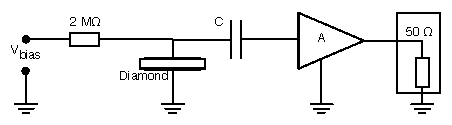
\includegraphics[width=0.8\textwidth]{03_measurement_results/plots/ro-chain}
\caption{Diagram of a diamond detector readout chain.}
\label{fig:ro-chain}
\end{figure}


\subsection{Preamplifiers}
\label{sec:preamps}
Two preamplifiers are used for the measurements, one sensitive to charge and the other to current. \emph{CIVIDEC Cx} (figure~\ref{fig:ampcx}) is a charge sensing amplifier. Its high SNR (equivalent noise charge of 300~+~30~pF$^{-1}$~e$^-$ and a reported gain of $\sim$12~mV/fC) makes it a good choice for spectroscopic measurements with diamond sensors. \emph{CIVIDEC C2} (figure~\ref{fig:ampc2}) is a fast current preamplifier with a 2~GHz bandwidth limit. It is used for TCT measurements because if its fast response and a good SNR. Both are embedded in an RF-tight aluminium box to reduce the noise pickup. Both have an AC coupled input and an output with a  50~$\Upomega$ termination.

\begin{figure}[!t]
%\centering
\begin{tabular}{cccc}
\subfloat[Cx charge sensing preamplifier]{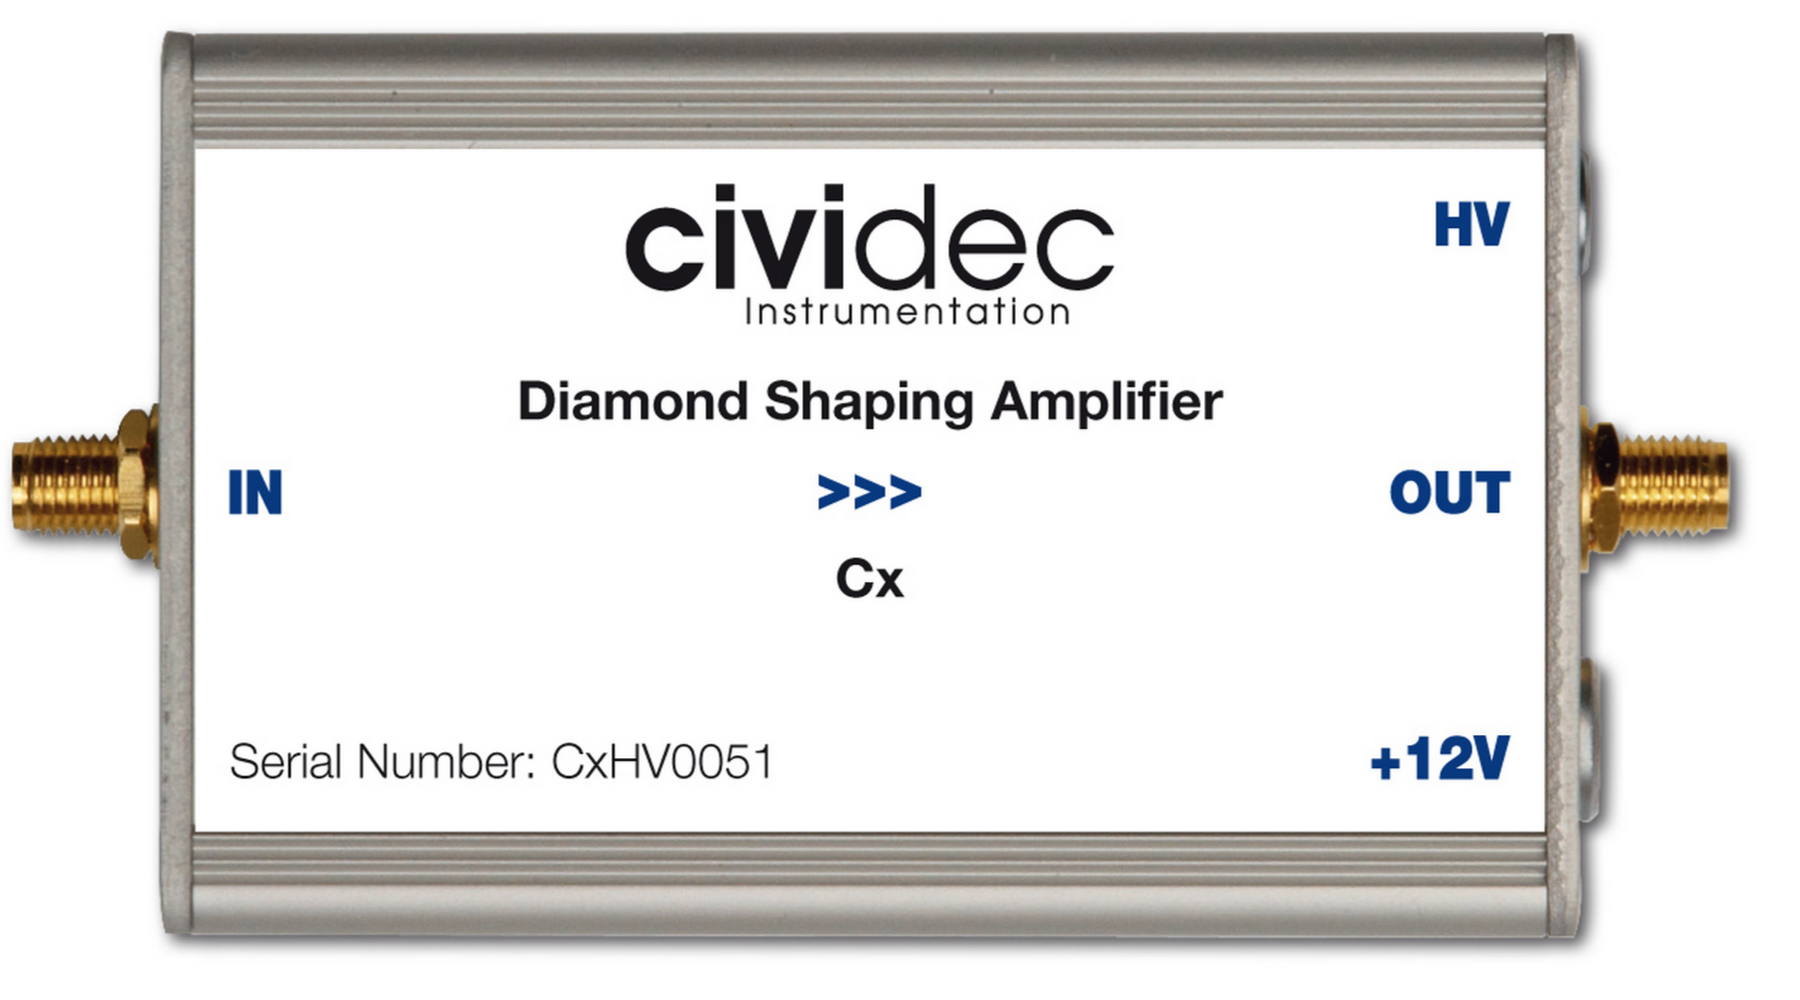
\includegraphics[width=0.47\textwidth]{03_measurement_results/pics/setup/Cx} \label{fig:ampcx}} &
\subfloat[C2 fast charge preamplifier]{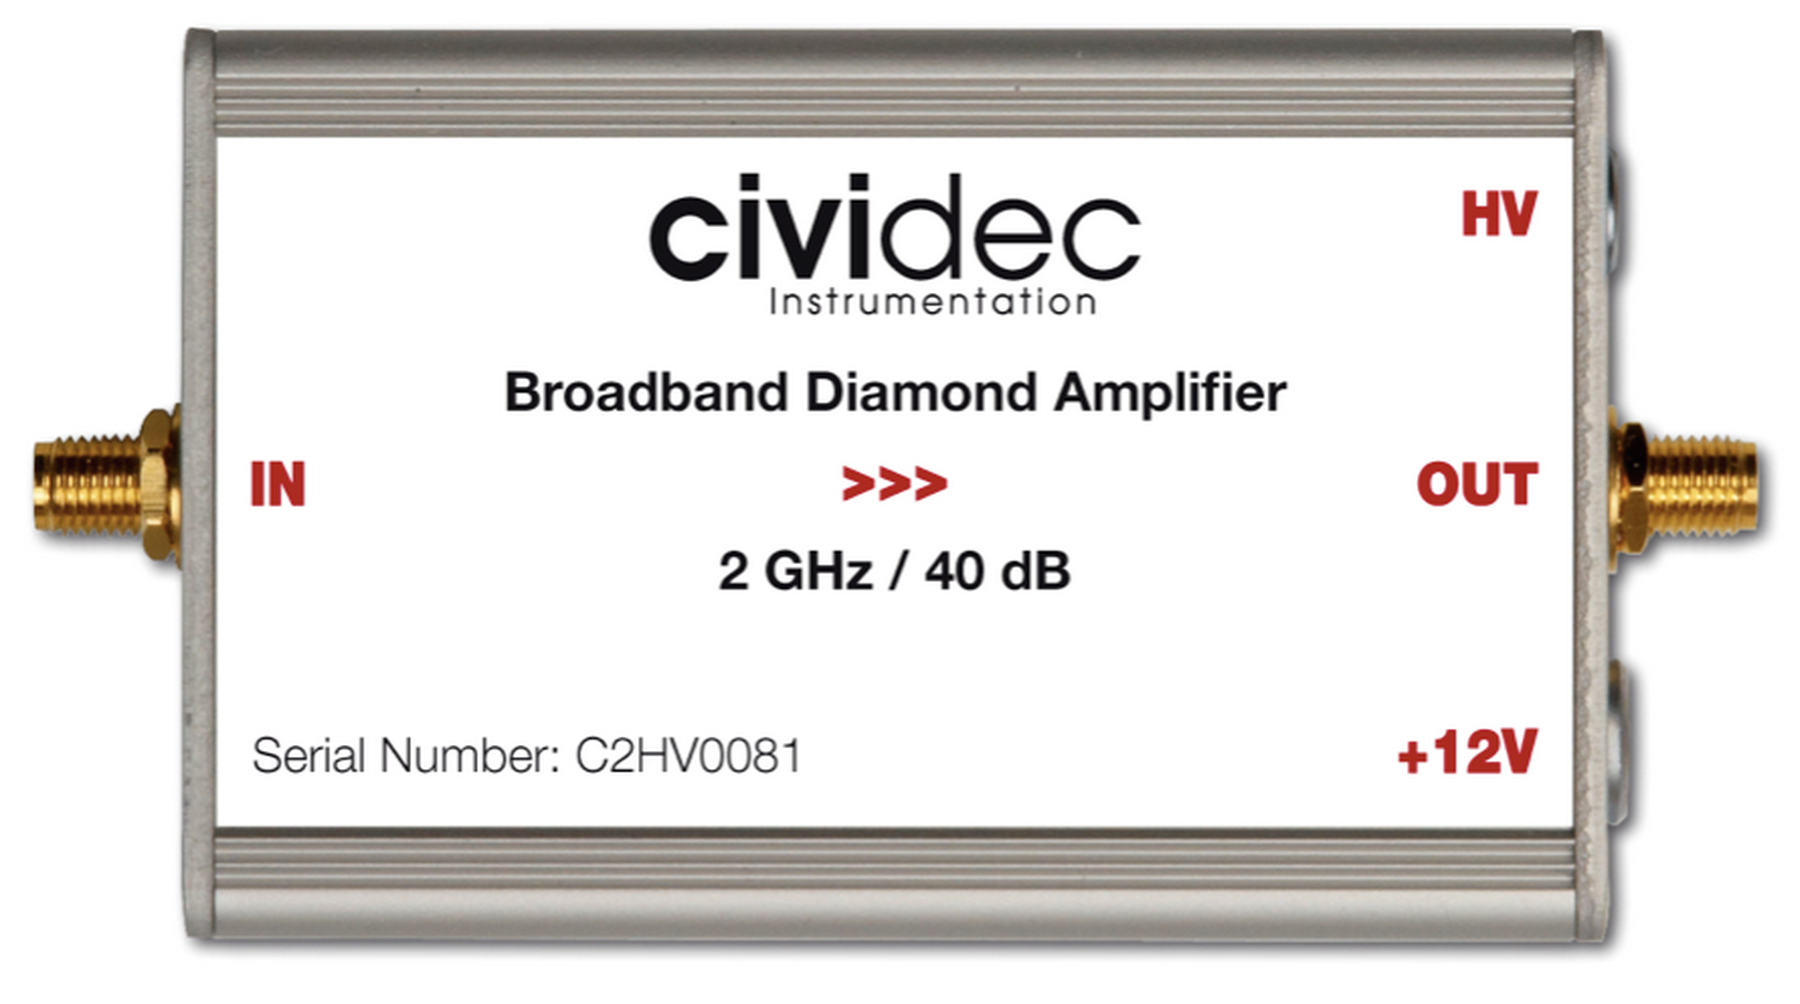
\includegraphics[width=0.47\textwidth]{03_measurement_results/pics/setup/C2}  \label{fig:ampc2}}
\end{tabular}
\caption{Amplifiers used for the charge and current measurements}
\end{figure}


\subsubsection{Calibration}
The amplifiers have to be calibrated before use to determine their gain. Both are calibrated using a square signal generator with a known amplitude step of $U_{\mathrm{in}}=(252\pm5)$~mV. A 2~GHz oscilloscope with a 10~GS/s sampling is used to carry out these measurements. 

In the case of the Cx charge sensitive amplifier, the signal is routed through a capacitor with a calibration capacitance $C_{\mathrm{cal}}=(0.717\pm0.014)$~pF and then to the input of the amplifier. The pulse area behind the capacitor is $a_{\mathrm{cal}}=(5.0\pm0.5)$~pVs, with the signal amplitude on the output amounting to $U_{\mathrm{C_x}}=(1.95\pm0.05)$~V. The input voltage step combined with the calibration capacitance yields a calibration charge $Q_{\mathrm{cal}}=C_{\mathrm{cal}}\cdot U_{\mathrm{in}}=(181\pm5)$~fC. The gain of the Cx amplifier is therefore $A^{\mathrm{Q}}_{\mathrm{Cx}}=\frac{U_{\mathrm{Cx}}}{Q_{\mathrm{cal}} }=(9.3\pm0.4)$~mV/fC or  $A^{\mathrm{a}}_{\mathrm{Cx}}=\frac{U_{\mathrm{Cx}}}{a_{\mathrm{cal}} }=(390\pm40)$~mV/pVs. The area-based amplification factor has a higher uncertainty ($\sim10~\%$) than the amplitude-based factor ($\sim4~\%$) due to the measurement limitations of the oscilloscope. Nevertheless, it can be used as an estimate for the integrated charge of a current pulse.

To calibrate the C2 current amplifier, only the amplitude gain has to be measured. The input signal amplitude has to be such that it keeps the output amplitude within the amplifier's linear range, that is $\pm1$~V. The signal from the generator is therefore routed through a 36~dB attenuator to decrease its amplitude to $U_{\mathrm{inAtt}}=(3.95\pm0.05)$~mV. Two amplifiers with different gains have been measured, because both are used for the measurements at different times. The output of the first amplifier amounts to $U_{\mathrm{C2-1}}=(860\pm5)$~mV. This yields the amplification gain equal to $A_{\mathrm{C2-1}}=\frac{U_{\mathrm{inAtt}}}{U_{\mathrm{C2-1}}} =(217\pm3)$. The second amplifier has the output equal to $U_{\mathrm{C2-2}}=(632\pm5)$~mV with the gain equal to $A_{\mathrm{C2-2}}=(152\pm3)$. 





\subsection{Diamond samples}
\label{sec:diamsam}
Detector-grade diamonds are very difficult to produce, mostly because it is very difficult to ensure a high enough purity of the lattice. %It takes companies years of trials to produce high enough quality product. Since the target market are almost exclusively particle physics research institutes, the companies work closely with them to make sure the product is up to par with the requirements. 
The sensor samples used for these studies were bought at Element Six (E6)~\cite{E6:00000}. They all have the same standard dimensions. sCVD diamonds with dimensions $4.7\times4.7$~mm$^2$ are already sufficiently large for most of the beam monitoring applications and still affordable. 
%; the cost of sCVD diamonds grows exponentially with the area. There is also an ongoing race among the producers to produce larger and larger diamonds while maintaining the same cost. For instance, a new company IIa~\cite{} from Singapore has produced high-quality samples with larger dimensions and the diamond detector community is currently involved in extensive tests of their products. 
One of the samples with dimensions of $5.6\times5.3$~mm$^2$ produced by IIa Singapore~\cite{IIA:00000} was also sent to CERN to be characterised. The target thickness for all the samples is 500~$\upmu$m. Diamonds this thick yield a high enough signal-to-noise ratio for MIPs to be measured by the electronics.
\begin{figure}
\centering
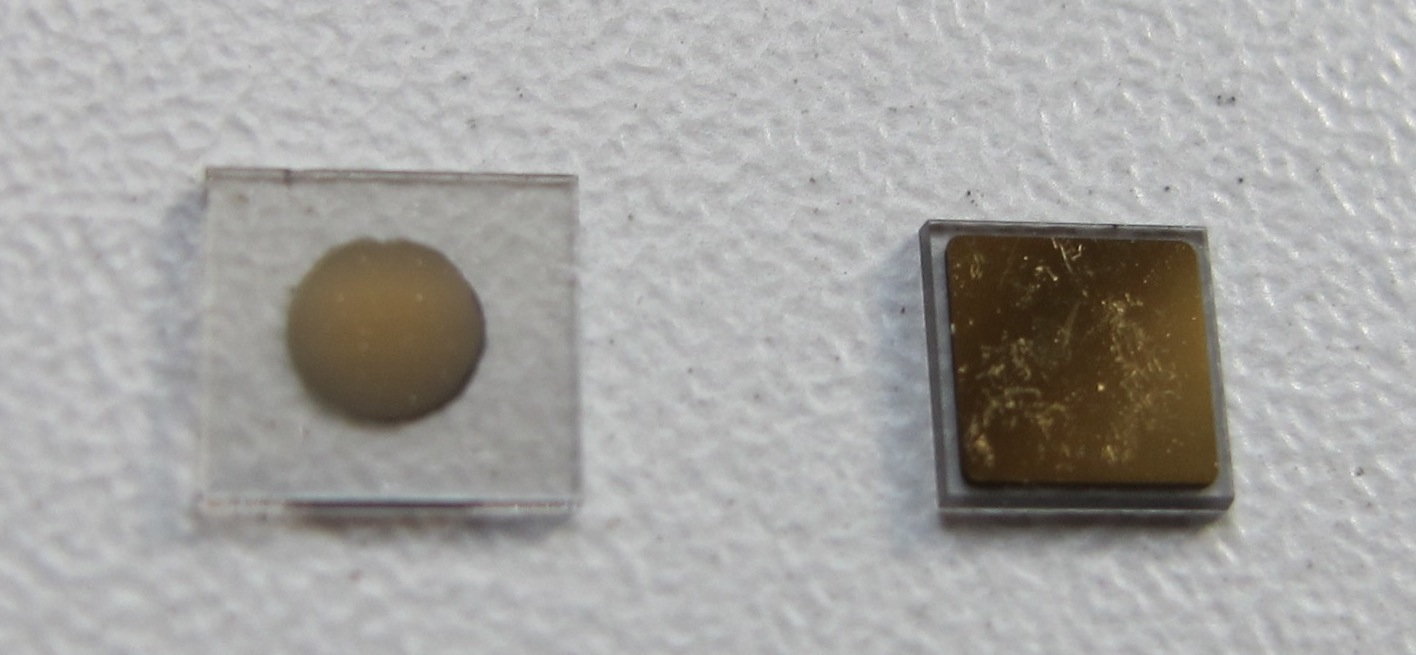
\includegraphics[width=0.8\textwidth]{03_measurement_results/pics/setup/diamond4}
\caption{Two scCVD diamond samples: A IIa 1scdhq (left) and an E6 S37 (right)}
\label{fig:diams}
\end{figure}
Table~\ref{tab:diamsamp} shows all the samples used for this study. Two of them were later irradiated with 300~MeV pions and then compared to the pre-irradiated state. Irradiation doses for damaging the material need to be high -- above $10^{12}$~particles per cm$^2$ to be able to observe change in the sensor's behaviour. 

\begin{footnotesize}
\begin{center}
\begin{tabular}{   l  c  c  c  c c c }
\hline
Name & Type &Producer & Dimensions [mm$^2$] & Thickness [$\upmu$m] & Electrode & Irradiatied \\
\hline
S37 & sCVD & E6 & $4.7\times4.7$ & 548 & Cr/Au & no \\
S50 & sCVD & E6 & $4.7\times4.7$ & 537 & Cr/Au & no \\
S52 & sCVD & E6 & $4.7\times4.7$ & 515 & Cr/Au & $1\times10^{14}~\uppi$~cm$^{-2}$ \\
S79 & sCVD & E6 & $4.7\times4.7$ & 529 & Cr/Au & $3.63\times10^{14}~\uppi$~cm$^{-2}$ \\
ELSC & sCVD & E6 & $4.7\times4.7$ & 491 & Cr/Au & no \\
1scdhq & sCVD & IIa & $5.6\times5.3$ & 460 & Cr/Au & no \\
\hline
\end{tabular}
\captionof{table}{Diamond sensor samples used}
\label{tab:diamsamp}
\end{center}
\end{footnotesize}
%_\mathrm{300~MeV}

The diamond samples have quoted impurity densities of $\leq2\times10^{14}$~cm$^{-3}$ and nitrogen incorporation of $\leq1$~ppb. The electrodes were added by various companies and institutes. For instance, S52 was metallised by a company DDL (now defunct) while the Physics Department of the University of Firenze, Italy metallised the S79. There are also several techniques for producing the electrodes. The DDL contacts consist of three layers: DLC (diamond-like carbon)/Pt/Au with 4/10/200 nm thicknesses, respectively. The metallisation for S79, on the other hand is made up of Cr/Au with a total thickness of $\sim$400~nm. The area coverage also differs from sample to sample. Diamonds must not be metallised until the very edge as the proximity of contacts with a high potential can lead to sparking. However, the areas not covered by the metallisation are less efficient because the fringe fields at the edges are not as strong as in the middle. This effectively reduces the sensitive area of the sensors. In the diamonds used here the effective area was anywhere from 9~mm$^2$ to 18~mm$^2$. Leakage current through the bulk was below 1~ns, but increased for the irradiated samples. The capacitance was of the order of (2.0$\pm$0.3)~pF.


\subsection{Readout devices}
\label{sec:readoutdev}
Electrical signals in diamond detectors are in the GHz frequency range. To preserve this information, the readout device has to have a high bandwidth limit. For instance, a 250~MHz limit is enough for the spectroscopic measurements with the Cx charge amplifier, but might be insufficient for the current measurements with the C2 amplifier. Two devices are used take data shown in this chapter. The first choice is a 2~GHz LeCroy WaveRunner 204MXi-A. This specific model has a high enough limit for the fast current preamplifier signals. It offers a versatile solution for analogue signal readout -- it is fast to set up and reliable. It is very convenient for use in lab tests and for experiments where small amounts of data are taken and where speed is not crucial. However, its slow acquisition speed turns out to be a bottleneck in the test beam experiment. Its initial 100~Hz readout rate decreases to a mere 20~Hz within 20 minutes, because every single trigger is saved as a separate file and the Windows operating system is not capable of handling 10000+ files in a single directory easily. This is why it has been exchanged with a DRS4~\cite{DRS4:00000}, an analogue readout device developed by PSI, Switzerland. This compact device is capable of recording up to four waveforms at a time at a steady rate of up to 500~Hz. Its 700~MHz bandwidth limitation is sufficient for the signal from the charge amplifier.



\subsection{Setup for the efficiency study using $\upbeta$ particles}
The efficiency study of the diamond sensors has been carried out at CERN in the North Hall test beam facility. There a straight high-energy particle beam of $\uppi_\mathrm{120~GeV}$ is provided to the users to calibrate their detectors. The beam had a transverse spread of $\sigma=10$~mm in both axes. The particle rate is of the order of $10^4~\uppi$~cm$^{-2}$~s$^{-1}$. A diamond sensor embedded in a PCB carrier has been placed in the beam spot perpendicular to the beam and connected via an SMA connector directly to a charge amplifier (described below). The amplified signal is read out using a LeCroy oscilloscope and a DRS4 analogue readout system (both described below). A computer is used as a controller and data storage for the readout device. A beam telescope is used as a reference detector. It is a device that helps to cross-check the measurements of the devices under test (DUTs) and to carry out spatially resolved studies on the DUTs. It consists of several pixellated sensor planes placed in series, which can track a particle's trajectory with a precision of a few $\upmu$m. The sensor planes are positioned in front of the DUT and behind it. Then the beam telescope acts as a trigger system -- it triggers the readout of both the telescope data and DUT data when both the planes in front and behind the DUT recorded a hit by the incident particle. A particle detected by all the planes within the DUT window and the DUT itself counts towards its efficiency whereas a hit missed by the DUT means that the DUT is not 100~\% efficient. To discard the hits that miss the DUT completely, a region of interest (ROI) can be chosen in the beam telescope planes. The equation for calculating the sensor efficiency is therefore
\begin{equation}
\label{eq:sensoreff}
\epsilon = \frac{ N_\mathrm{DUT} \wedge N_\mathrm{telescope} }{ N_\mathrm{telescope} }
\end{equation}
for an ROI smaller than the sensitive region of the diamond.


\subsection{Room temperature $\upalpha$-TCT setup}
This TCT study is a follow-up of an extensive diamond TCT study at cryogenic temperatures~\cite{Jansen:1956431}. The room-temperature TCT measurements have been carried out in the lab. The setup consists of a diamond sensor embedded in a PCB carrier, a current amplifier and an oscilloscope. To measure $\upalpha$ particles, their energy loss during their trajectory has to be minimised. Therefore the diamond is placed inside a vacuum chamber. The chamber is a steel tube with a diameter of 5~cm. On one side it is connected to a vacuum pump via an steel pipe. A feedthrough with an SMA connector is placed on the other side. A C2 current amplifier is connected directly onto the feedthrough. The amplified output is connected to the oscilloscope via an SMA cable. An $^{241}$Am source with a diameter of 2~cm and a height of 0.5~cm is fixed onto the sensor carrier (figure~\ref{fig:carrier}, figure~\ref{fig:carsrc}). Then the carrier is inserted in the chamber and fixed in place using an air-tight clamp. The pump can then be switched on. It is capable of providing the inside pressure as low as $10^{-4}$~mbar after approximately one hour of operation, but measurements can take place even after five minutes of evacuation, at around $10^{-3}$~mbar. The most important thing to bear in mind is to switch the bias voltage of the sensor OFF during the process of evacuation, because the gas becomes more conductive at the pressure of the order of $10^{-1}$~mbar, which is at the bottom of Paschen's curve~\cite{PASCHEN:00000}. A failure to switch off the bias voltage may cause a spark between the signal and ground line, destroying the amplifier. 

\begin{figure}[!t]
%\centering
\begin{tabular}{cccc}
\subfloat[PCB carrier with an embedded diamond sample]{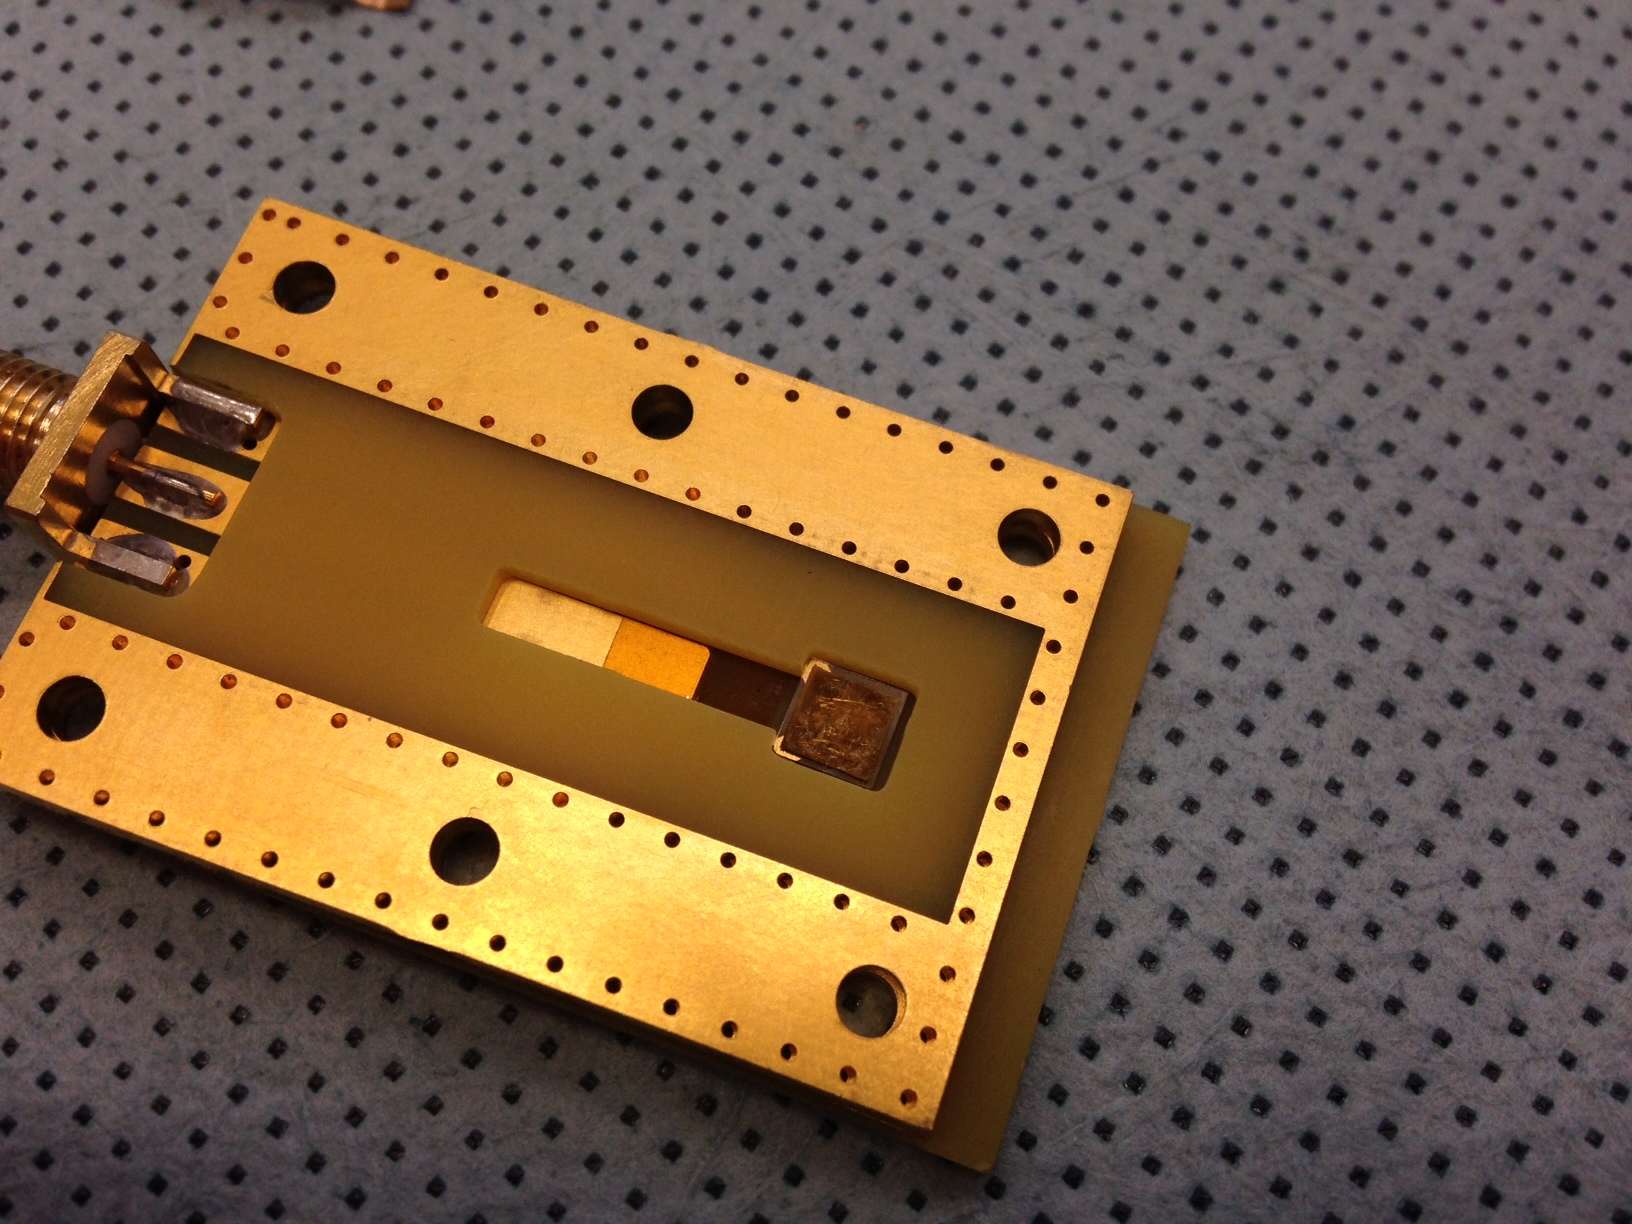
\includegraphics[width=0.47\textwidth]{03_measurement_results/pics/setup/carrier2} \label{fig:carrier}} &
\subfloat[Radioactive source over the carrier]{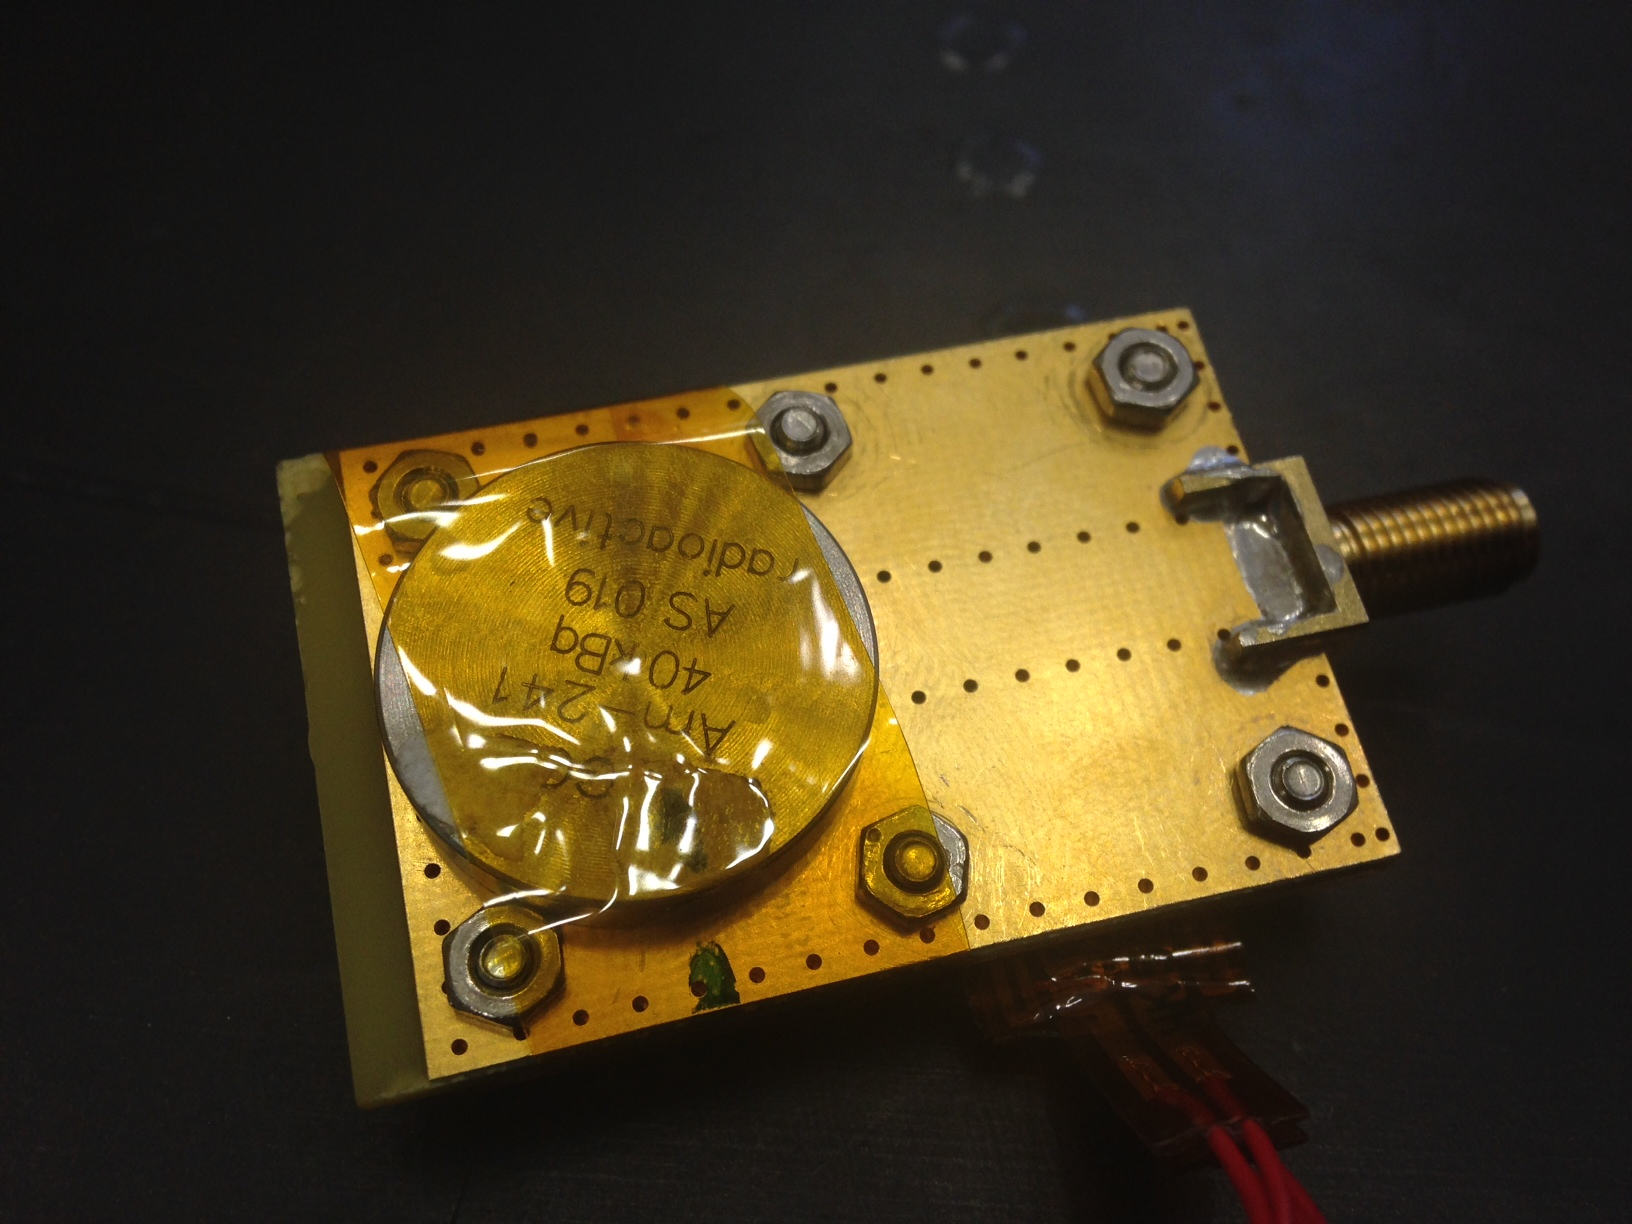
\includegraphics[width=0.47\textwidth]{03_measurement_results/pics/setup/carriersource2}  \label{fig:carsrc}}
\end{tabular}
\caption{Positioning of the $\upalpha$-source on top of the sensor carrier}
\end{figure}


\subsection{Cryogenic $\upalpha$-TCT setup}
\label{sec:cryosetup}
The experiment at cryogenic temperatures has been carried out in the cryolab at CERN. The room-temperature TCT setup has to be modified to allow for measurements at temperatures as low as 2~K. It consists of three parts: 
\begin{enumerate}
\item a cryostat --  a thermally insulated cylinder capable of containing liquid helium,
\item an inlet -- an air-tight mechanical tube with valves and feedthroughs at the top that is lowered in the liquid helium and
\item the diamond sample embedded in a PCB carrier with a fitted temperature sensor, a heater and cables leading to the feedthroughs.
\end{enumerate}
The setup is described in detail in~\cite{Jansen:1956431}.

When the diamond sample is placed in the PCB carrier and the $^{241}$Am source is in place, the inlet is sealed and lowered in the empty cryostat. Then the inside volume of the inlet is evacuated to down to $10^{-5}$~mbar while the liquid helium is flowing into the cryostat. To improve the thermal contact between the diamond and the coolant, a small amount of helium gas is added inside the evacuated inlet, setting the vacuum to around $10^{-3}$~mbar. This value changes with time, because the gas condenses on the walls of the inlet, reducing the number of floating particles. For this reason the helium gas has to be added on an irregular basis. Every addition causes a significant undershoot of the sample temperature, which had to be corrected for using a heater placed on the back of the PCB carrier. Also, the added gas deteriorates the vacuum inside the inlet. It is very important to monitor the pressure so as not to let it rise above $10^{-2}$~mbar. The gas at this pressure is significantly more conductive and could cause a short circuit between the two diamond plates or in the SMA connectors, destroying the amplifier. Furthermore, at approximately 60~K the helium gas has to be evacuated from the inlet to avoid a potential explosion due to the expansion of the gas with temperature. 

When the sample is cooled to the minimum temperature achievable by means of liquid helium without over-pressurising it (4.2~K), the measurements start. A temperature sensor placed on the back of the PCB carrier is used to measure the temperature of the sample. After every temperature data point, the current through the heater placed in the PCB next to the diamond sample is increased, warming up the sample. The initial temperature time constant of the order of tenths of seconds at low temperatures increases with temperature. Even more so when helium is evacuated from the inlet at 60~K, removing the thermal bridge between the wall of the inlet and the diamond sample. At the room temperature (RT), the time constant increases to the order of minutes.







%TCT, testbeam DISCUSSED IN CHAPTER 2!!!!!



% ---------------------------------------------------------------------------------------------------------------
%\clearpage
\section{Charged particle pulses and spectra}
\label{sec:pulsespectra}
% ---------------------------------------------------------------------------------------------------------------
In previous chapter the ionisation profiles for different types of radiation were discussed. It is known that $\upbeta$ and $\upgamma$ radiation induces a triangular electric pulse whereas $\upalpha$ radiation induces a rectangular one. However, their amplitude, width and rise/fall time depend heavily on the type of interaction with the diamond, the purity of the diamond and the bandwidth of the amplifier and the oscilloscope. This section shows the signal pulses of $\upalpha, \upbeta$ and $\upgamma$ radiation with their respective energy distributions for the case of a diamond detector. Then follows a discussion of effects of noise on these measurements. 

A CIVIDEC C2 current amplifier together with the LeCroy oscilloscope (both with a bandwidth limit of 2~GHz) has been used to record the pulse shapes whereas the Cx charge amplifier is used for charge measurement. A 2~GHz bandwidth limit defines the minimum rising time equal to $t_{\mathrm{r}}\simeq\frac{0.34}{BW}=\frac{0.34}{2\times10^9}=170$~ps, therefore the system is capable of measuring pulses with a minimum FWHM$\simeq170~ps$. This already makes it impossible to measure the initial peak in the $\upalpha$ response due to the two flavours of charge carriers travelling. If a charge carrier travelling through the bulk takes $t_{\mathrm{t1}}\sim~$6~ns to get to the electrode on the other side (d$_\mathrm{1}\sim500~\upmu m$), the carrier with the opposite charge and a shorter path to the closer electrode -- max. d$_2\sim10~\upmu$m -- only takes $t_{\mathrm{t2}}\sim \frac{d_\mathrm{2}}{d_\mathrm{1}}t_{\mathrm{t1}}=120$~ps. A drift time this short induces a current pulse that is too narrow for the C2 amplifier or the oscilloscope to be able to observe.

Figure~\ref{fig:pulsesaby} shows a set of pulses and an averaged pulse for $\upalpha, \upbeta$ and $\upgamma$ radiation using an $^{241}$Am, $^{90}$Sr and $^{60}$Co source, respectively. The particles are measured with the non-irradiated sCVD diamond S37. $\upalpha$ particles always produce the same signal pulse, but with a high noise RMS. The averaging suppresses the noise while still retaining most the information. It does, however, smear the rising and falling edge, increasing the rise time. The t$_{\mathrm{r}}$ is now of the order of 0.5~ns. Both $\upbeta$ and $\upgamma$ pulses look similar - triangular and with a wide range of amplitudes. Here the pulse count is low, so the pulses with a high amplitude are not recorded. A trigger set very high would be needed to ``catch'' them with the oscilloscope.

\begin{figure}[!t]
\centering
\begin{tabular}{rrr}
\subfloat{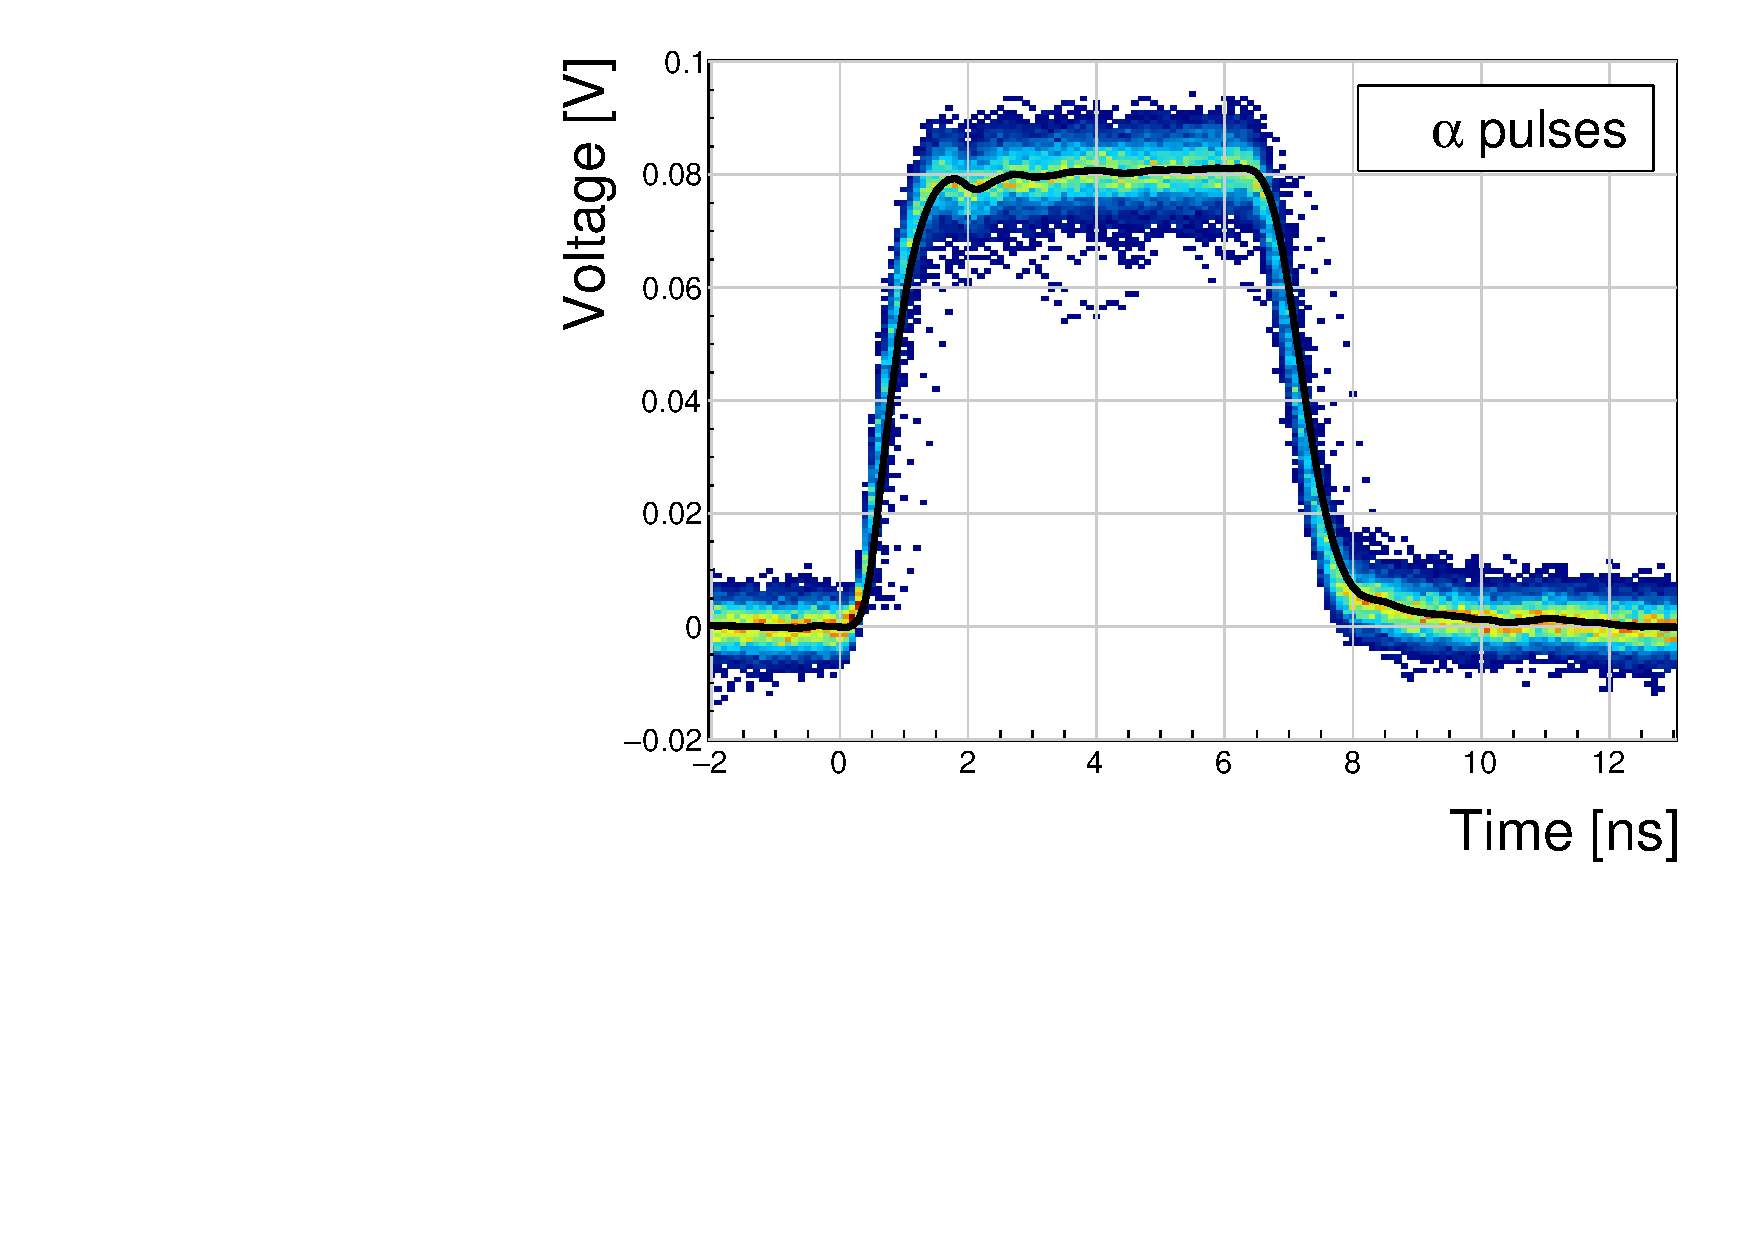
\includegraphics[width=0.47\textwidth]{03_measurement_results/scripts/plots/samplePulses/alpha} \label{fig:alpha1}} &
\subfloat{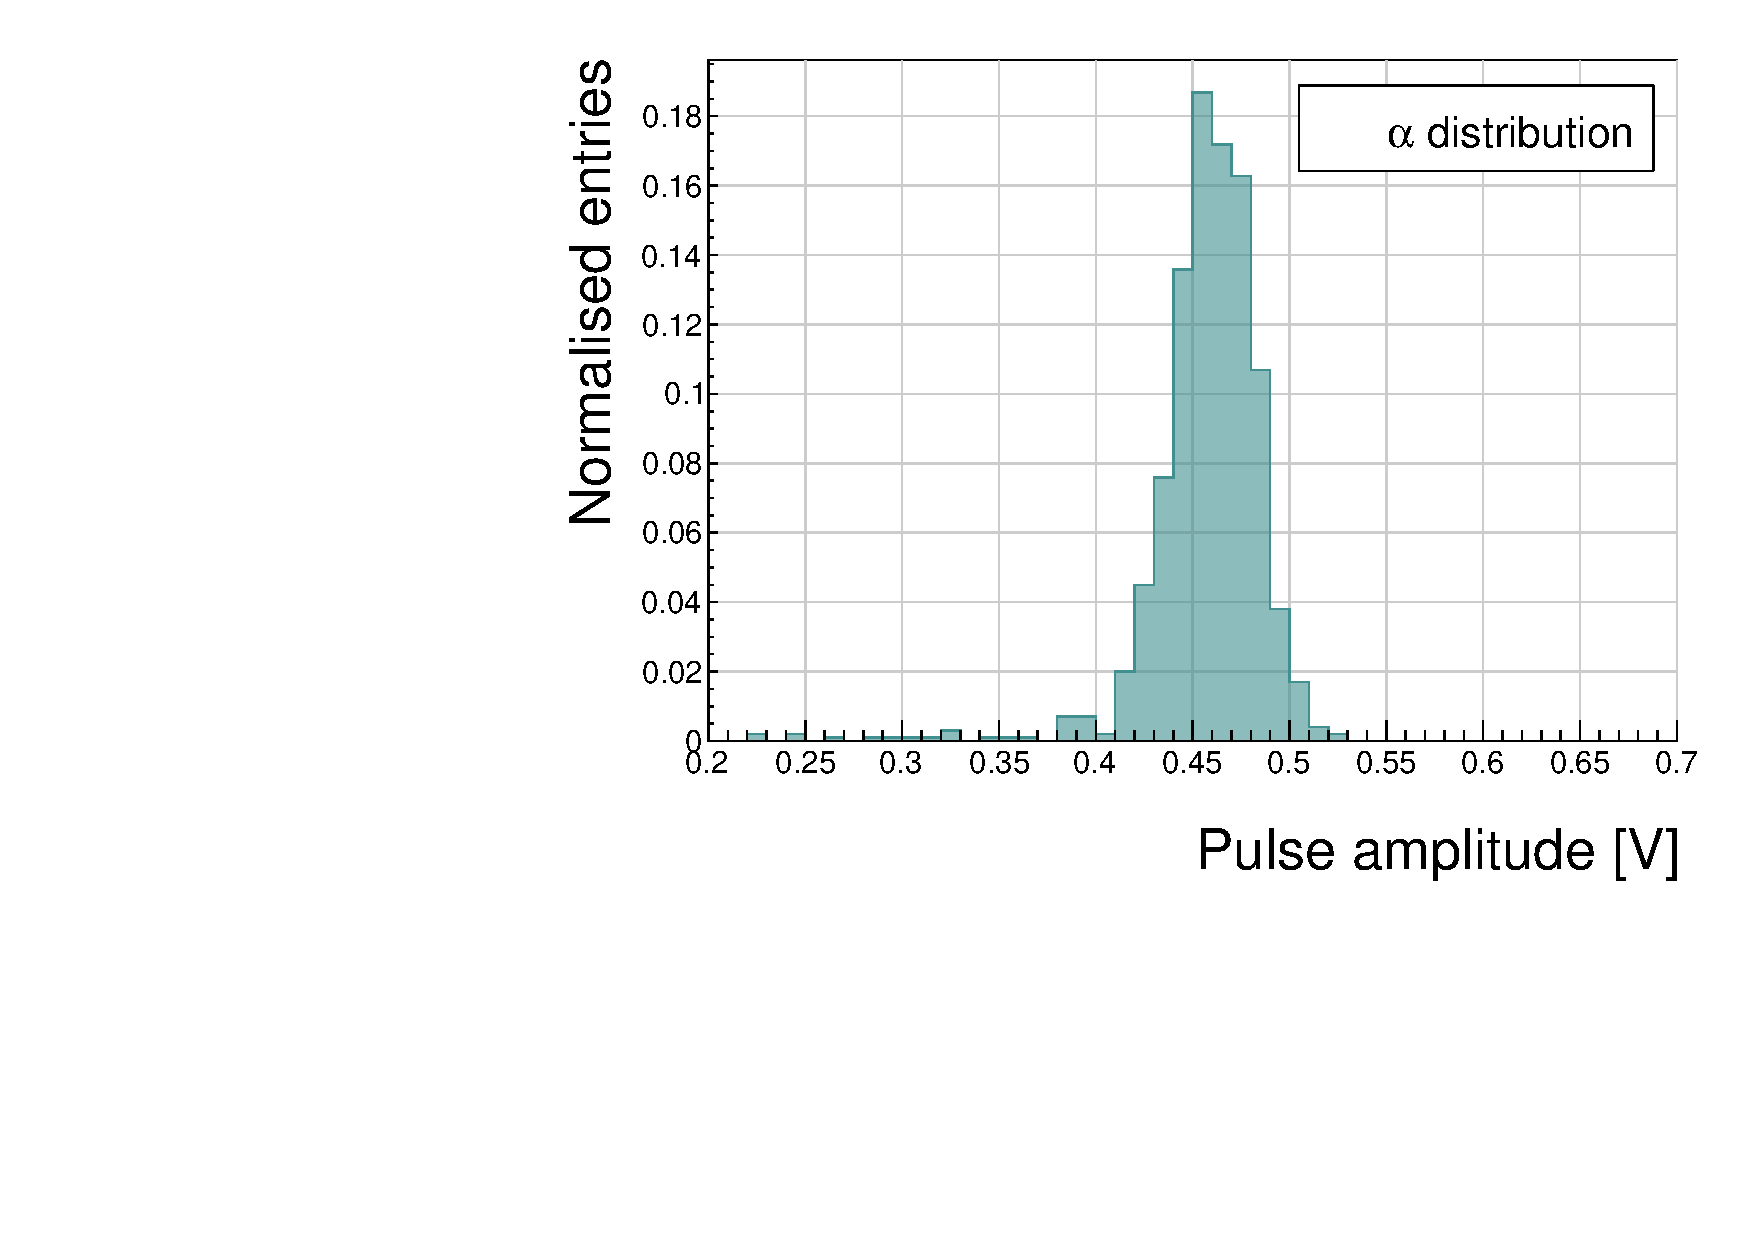
\includegraphics[width=0.47\textwidth]{03_measurement_results/scripts/plots/samplePulses/alphadist} \label{fig:alphadist1}} \\
\subfloat{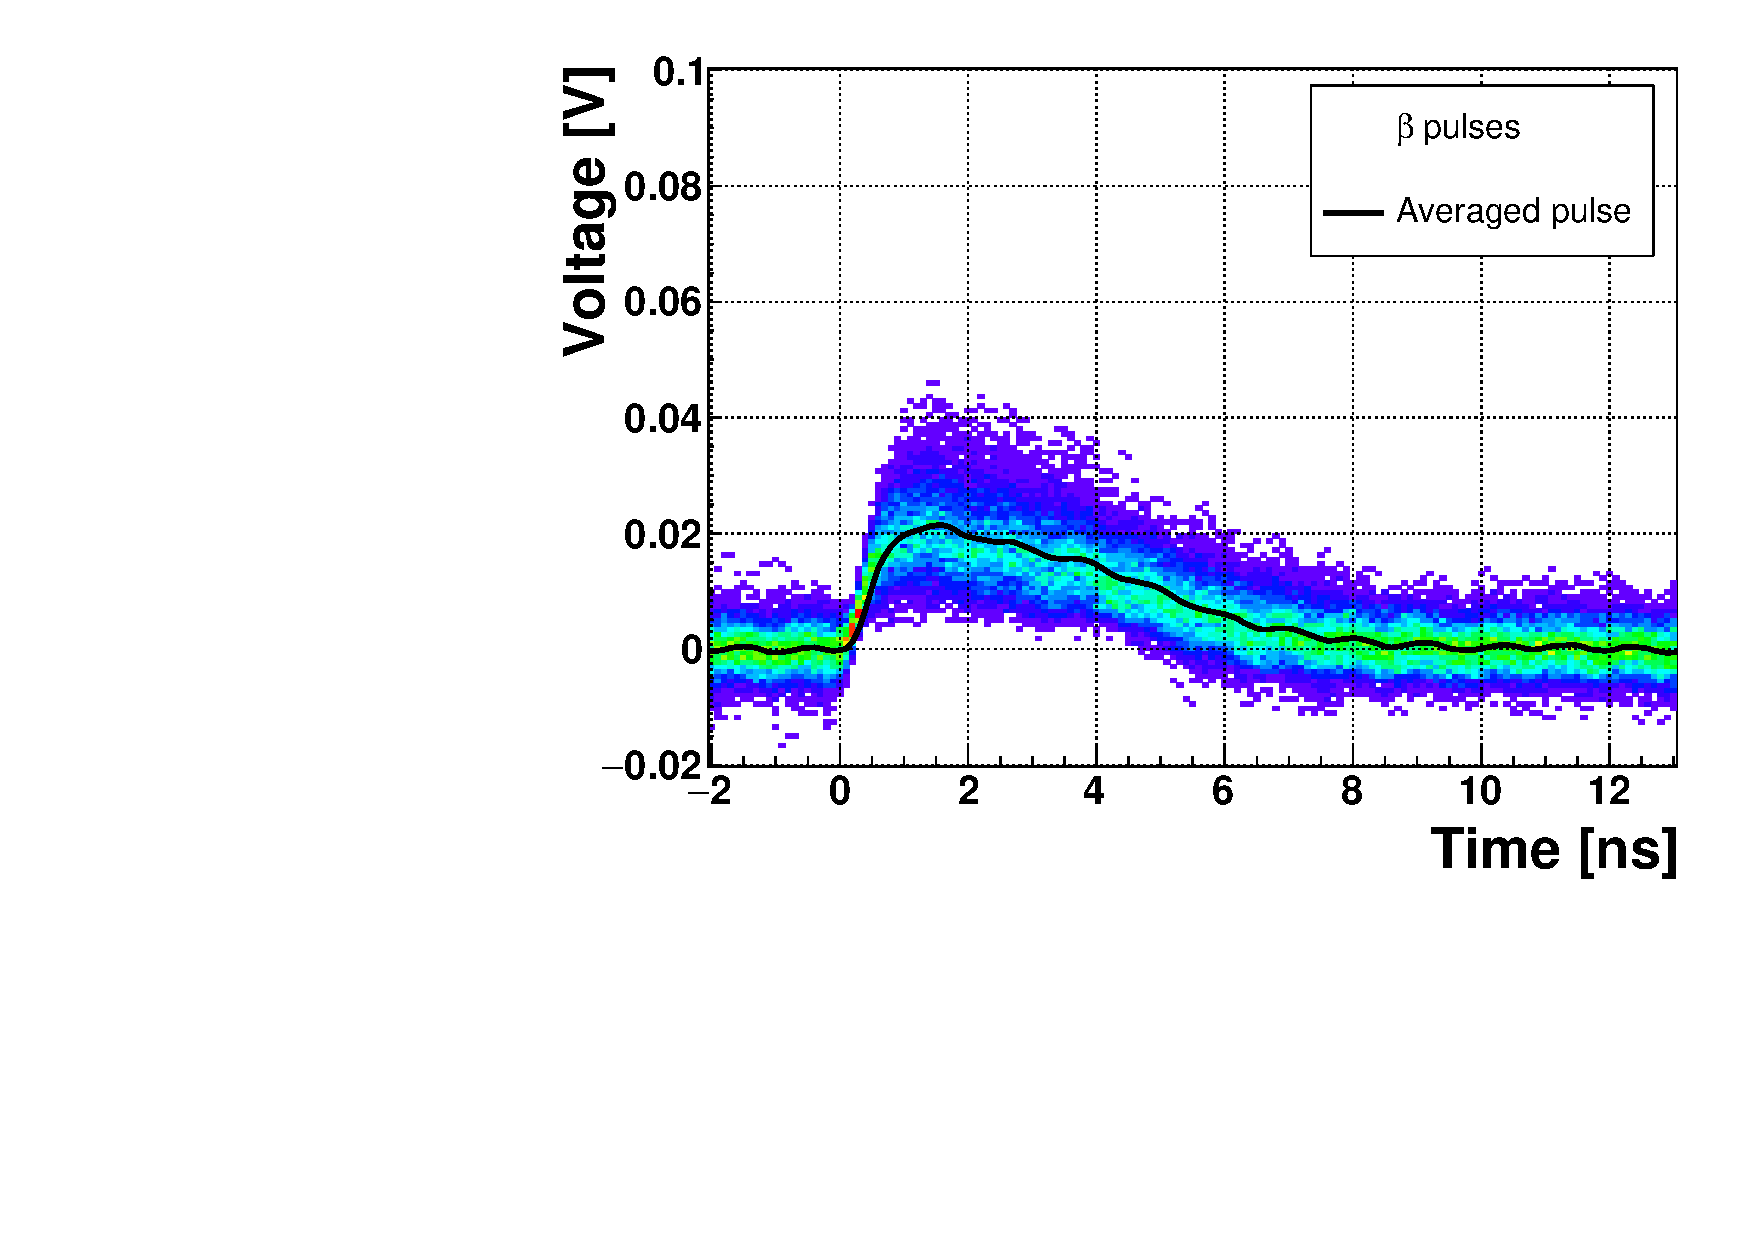
\includegraphics[width=0.47\textwidth]{03_measurement_results/scripts/plots/samplePulses/beta}  \label{fig:beta1}} &
\subfloat{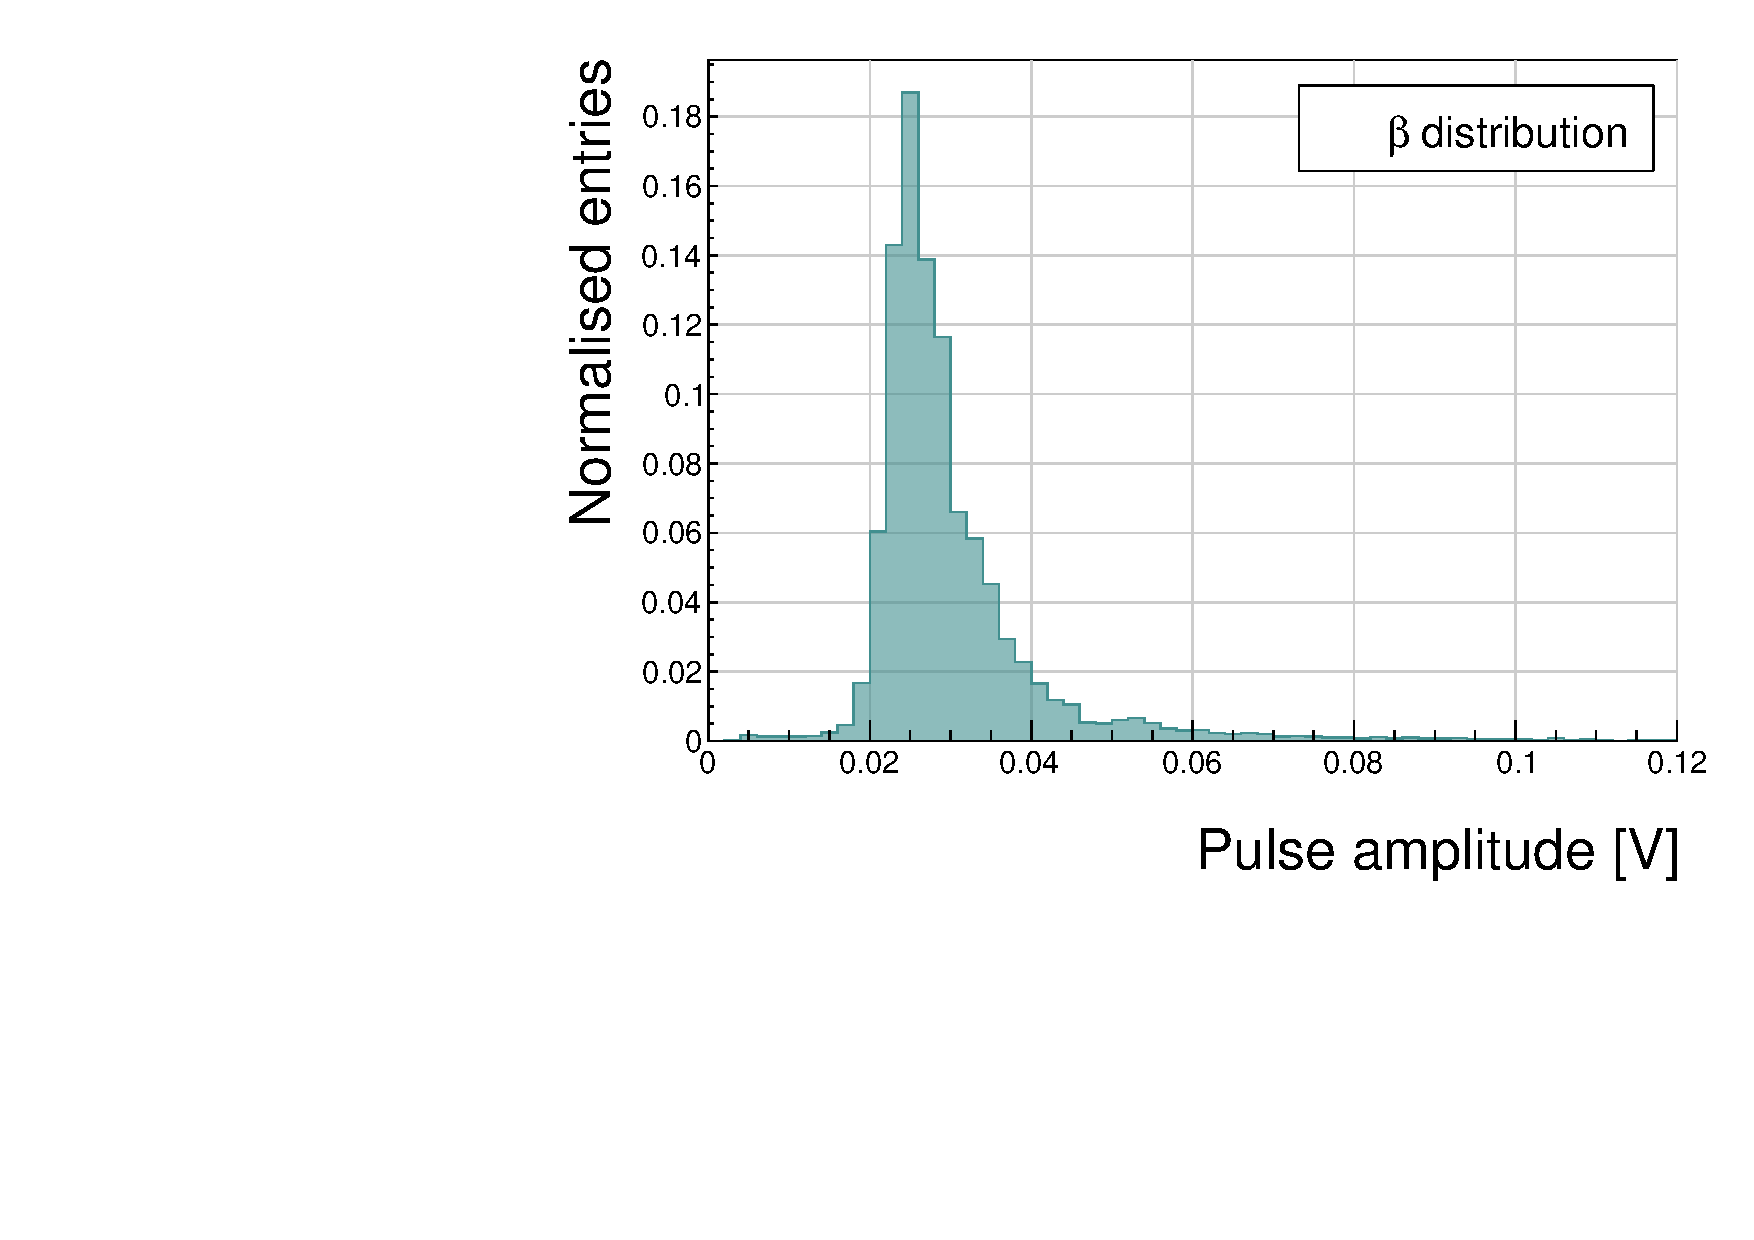
\includegraphics[width=0.47\textwidth]{03_measurement_results/scripts/plots/samplePulses/betadist}  \label{fig:betadist1}} \\
\subfloat{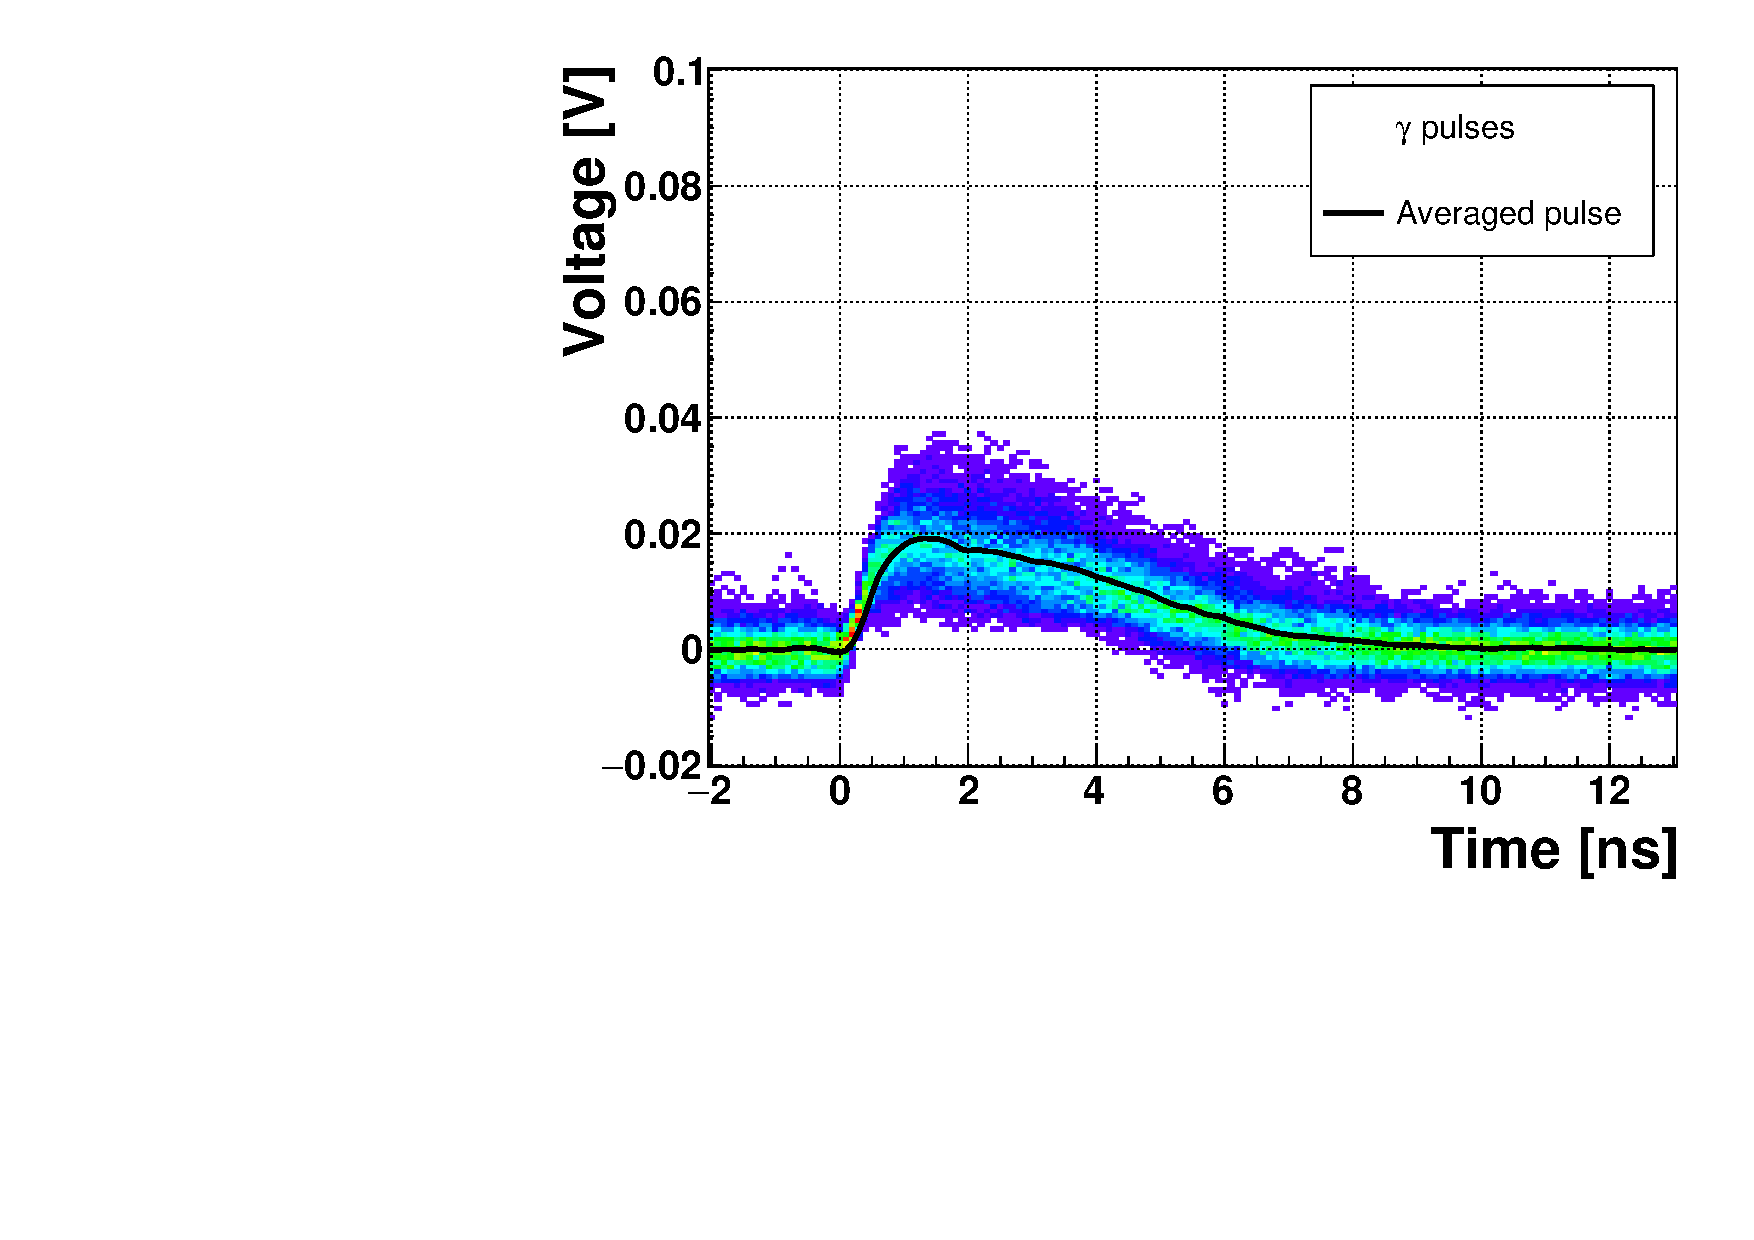
\includegraphics[width=0.47\textwidth]{03_measurement_results/scripts/plots/samplePulses/gamma}  \label{fig:gamma1}} &
\subfloat{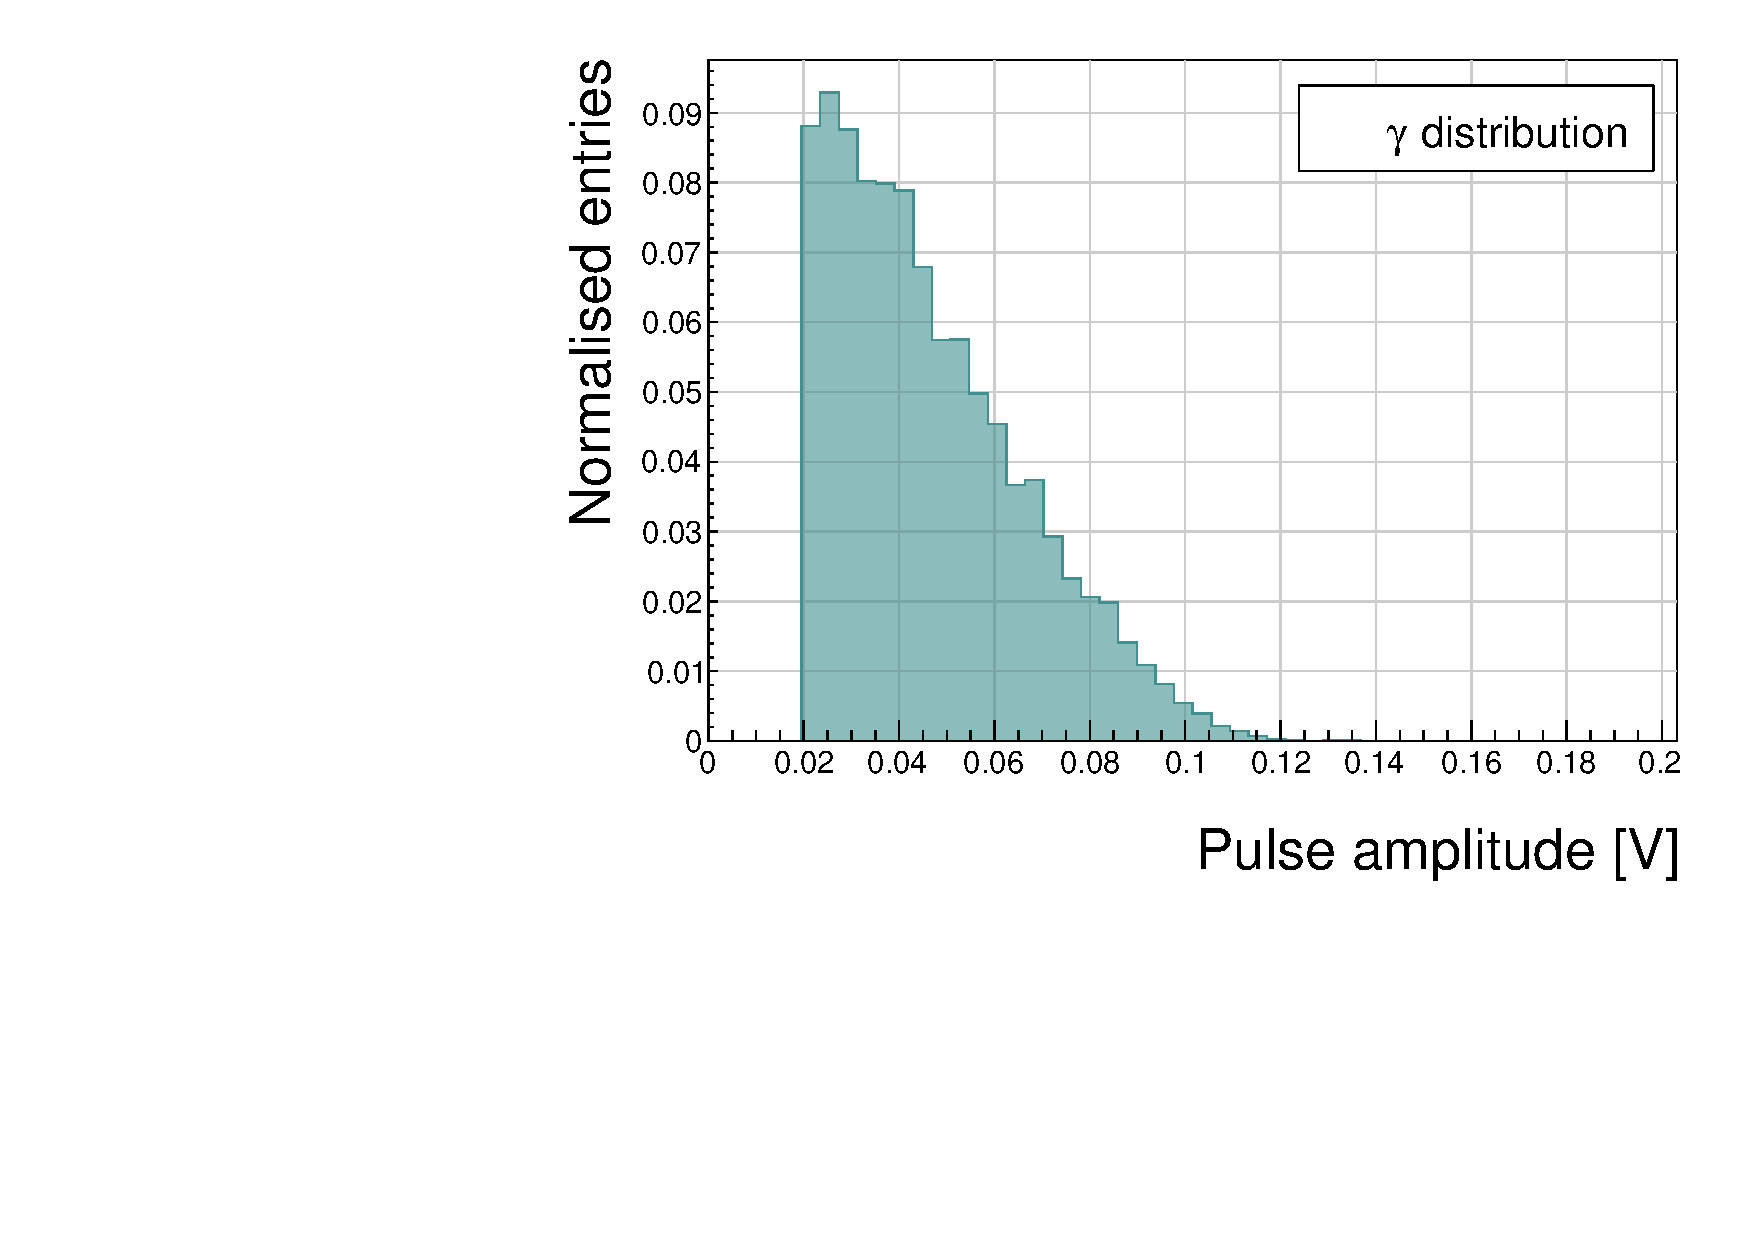
\includegraphics[width=0.47\textwidth]{03_measurement_results/scripts/plots/samplePulses/gammadist}  \label{fig:gammadist1}} 
\end{tabular}
\caption{Superimposed and averaged pulses (a, b and c, current amplifier) and distributions of deposited energy (d, e, f, charge amplifier) for three types of radiation. Note the scale on the X axis of the distributions.}
\label{fig:pulsesaby}
\end{figure}




%---------------------------------------------------------------------------------------------------------------
%%\clearpage
\subsection{Noise limitations}
\label{sec:noiselimit}
%---------------------------------------------------------------------------------------------------------------
%TO DO: Take 8 runs with the 2GHz oscilloscope while increasing the noise. 
%TO DO: leakage current, irradiated.
Noise is a major limiting factor in particle detection. It defines the minimum measurable particle energy and the minimum measurement resolution. It is hence important to minimise the electric noise in the detector signal. The major noise contribution comes from poor shielding from external electromagnetic sources. These often cause ringing, whereby the signal oscillates with a frequency defined by the external source. The ringing makes high-frequency measurements impossible. Another source of noise is the sensor itself. In the case of silicon, natural light increases the number of thermally excited free charge carriers, increasing the leakage current. This is not the case for diamond, which is with its high energy band gap insensitive to visible light. Nevertheless, any noise produced by the sensors is amplified by the signal amplifiers, which add an additional noise of the analogue electrical circuit to the amplified signal. Finally, the digitisers add the quantisation noise to the digitised signal. If the measurement range is significantly higher than the actual measured signal, the quantisation noise can be a significant contributor to the decrease of the overall measurement resolution.






% ---------------------------------------------------------------------------------------------------------------
%\clearpage
\section{Radiation limitations}
\label{sec:radlimit}
% ---------------------------------------------------------------------------------------------------------------
Exposure to ionising radiation degrades sensors. It deforms the lattice by displacing the atoms. Various types of lattice defects can be created in diamond, similar to those in silicon: vacancies, interstitials etc.~\cite{CHTR:00000} These deformations introduce new discrete energy levels between the valence and conduction band. Charge carriers drifting in their vicinity can get trapped, their energy falling to the energy level of the trap. Their emission back to the conduction band depends on how deep the trap is (how far away from the conduction band it is). The carriers caught in the shallow traps of the order of 100~meV below the conduction band are excited back up already by means of the thermal excitation. This phenomenon has a short time constant, dependant on the environmental temperature. Those stopped by deep traps near the middle of the band gap need more energy and thus more time to be emitted to either the conduction or valence band. Some charge carriers remain trapped for long periods. If they build up in a certain region of the diamond, their charge starts affecting the surrounding electric field -- space-charge forms. It can either help or counteract the field, depending on the polarity of the carrier. 

The energy band jumping goes the other way, too. The carriers in the valence band may use the intermediate energy levels as ``stepping stones'' to jump to the conduction band and start drifting in the externally applied electric field. This is called the leakage current.

The electrons and holes stopped in these traps cause a decrease of the induced current on the electrodes. This yields a lower integrated charge in an irradiated sensor than that in a non-irradiated one. Charge collection efficiency is therefore correlated with the level of irradiation. 

This section contains a study of the effects of pion ($\uppi_{\mathrm{300~MeV}}$) irradiation on the charge collection efficiency of sCVD diamond detectors. To carry out this study, two diamond samples have been irradiated to doses of 1$\times10^{14}~\pi$~cm$^{-2}$ (S79) and to 3.63$\times10^{14}~\pi$~cm$^{-2}$ (S52). Then a test beam campaign has to be carried out to observe the charge collection efficiency at different bias voltage settings. The efficiency values acquired are used to determine the effective drop in efficiency with respect to received radiation dose. This is to test if the collected charge $Q$ is inversely proportional to the received dose $\Phi$. A procedure defined by a collaboration researching diamond behaviour RD42 has been applied to the measured values to extract the damage factor. The next subsection contains measurements and results of a long-term stability study using $\upalpha$ and $\upbeta$ particles. In particular, the charge collection efficiency as a function of time is measured during the measurements with $\upbeta$ and $\upalpha$ radiation. To investigate this effect on the scale of charge carriers, the change of TCT pulses with time is observed. Finally, a procedure that improves the pulse shape and with it the charge collection is proposed.

\subsection{Quantifying radiation damage in diamonds}
Radiation damage varies with the type of radiation (particles or photons) and its energy. There are several models existing~\cite{2002NIMPA,Guthoff:2014223} that try to explain the impact of irradiation and to provide \emph{hardness factors} to compare the radiation damage between different particles. The standard way is to convert the damage into \emph{neutron equivalent}~\cite{NEQ:00000}. Some models have been extensively verified with simulations and with experiments. In these experiments charge collection in sensors is measured before and after irradiation. This procedure is repeated several times, with a measurement point taken after every irradiation. When a set of measurements of charge collection is plotted against the radiation dose received by a specific particle at a specific energy, a damage factor $k_\mathrm{\lambda}$ can be extracted. Damage factors have to be measured across a range of energies and types of radiation to properly quantify the damage in the sensors. They are then compared against the simulations to verify that the experimental observations are in line with the theory.

Diamond is an expensive material and the technology is relatively new as compared to silicon. Therefore not many institutes are carrying out diamond irradiation studies. To join the efforts, the RD42 collaboration~\cite{RD42:00000} was formed. It gathers the experimental data from diamond irradiation studies. Unlike with silicon, the experimental results so far show no significant correlation with the NIEL (non-ionising energy loss) model~\cite{2002NIMPA}, which correlates detector efficiency with the number of lattice displacements. Therefore an alternative model was proposed~\cite{Guthoff:2014223}, correlating the diamond efficiency with the number of displacements per atom (DPA) in the bulk. The idea is that if the recoil energy of an incident particle is higher than the lattice binding energy (42~eV for diamond), the atom is displaced from its original position. The newly formed vacancy acts as a trap for drifting charge carriers. The more displacements that form in the bulk, the higher is the probability that a drifting carrier will get trapped, effectively reducing the induced signal. However, different types of particles interact differently with the bulk. In addition the mechanisms of interaction at low energies are different to those at high energies. To assess the damage for individual particles at a range of energies, simulations need to be run first. The simulation shown in~\cite{Guthoff:2014223} shows the DPA model for a range of energies of proton, pion and neutron irradiation in diamond. Figure~\ref{fig:kitdpa}  contains the simulation results as well as the superimposed empirical results of several irradiation studies. According to the figure, a 300~MeV pion beam damages the diamond bulk twice as much as a 24~GeV proton beam. The data points obtained by RD42 are also added to the figure. They have been normalised to damage by 24~GeV protons. Finally, the data point measured in the scope of this thesis has been added for comparison. The derivation is done below.

\begin{figure}[!t]
\begin{center}
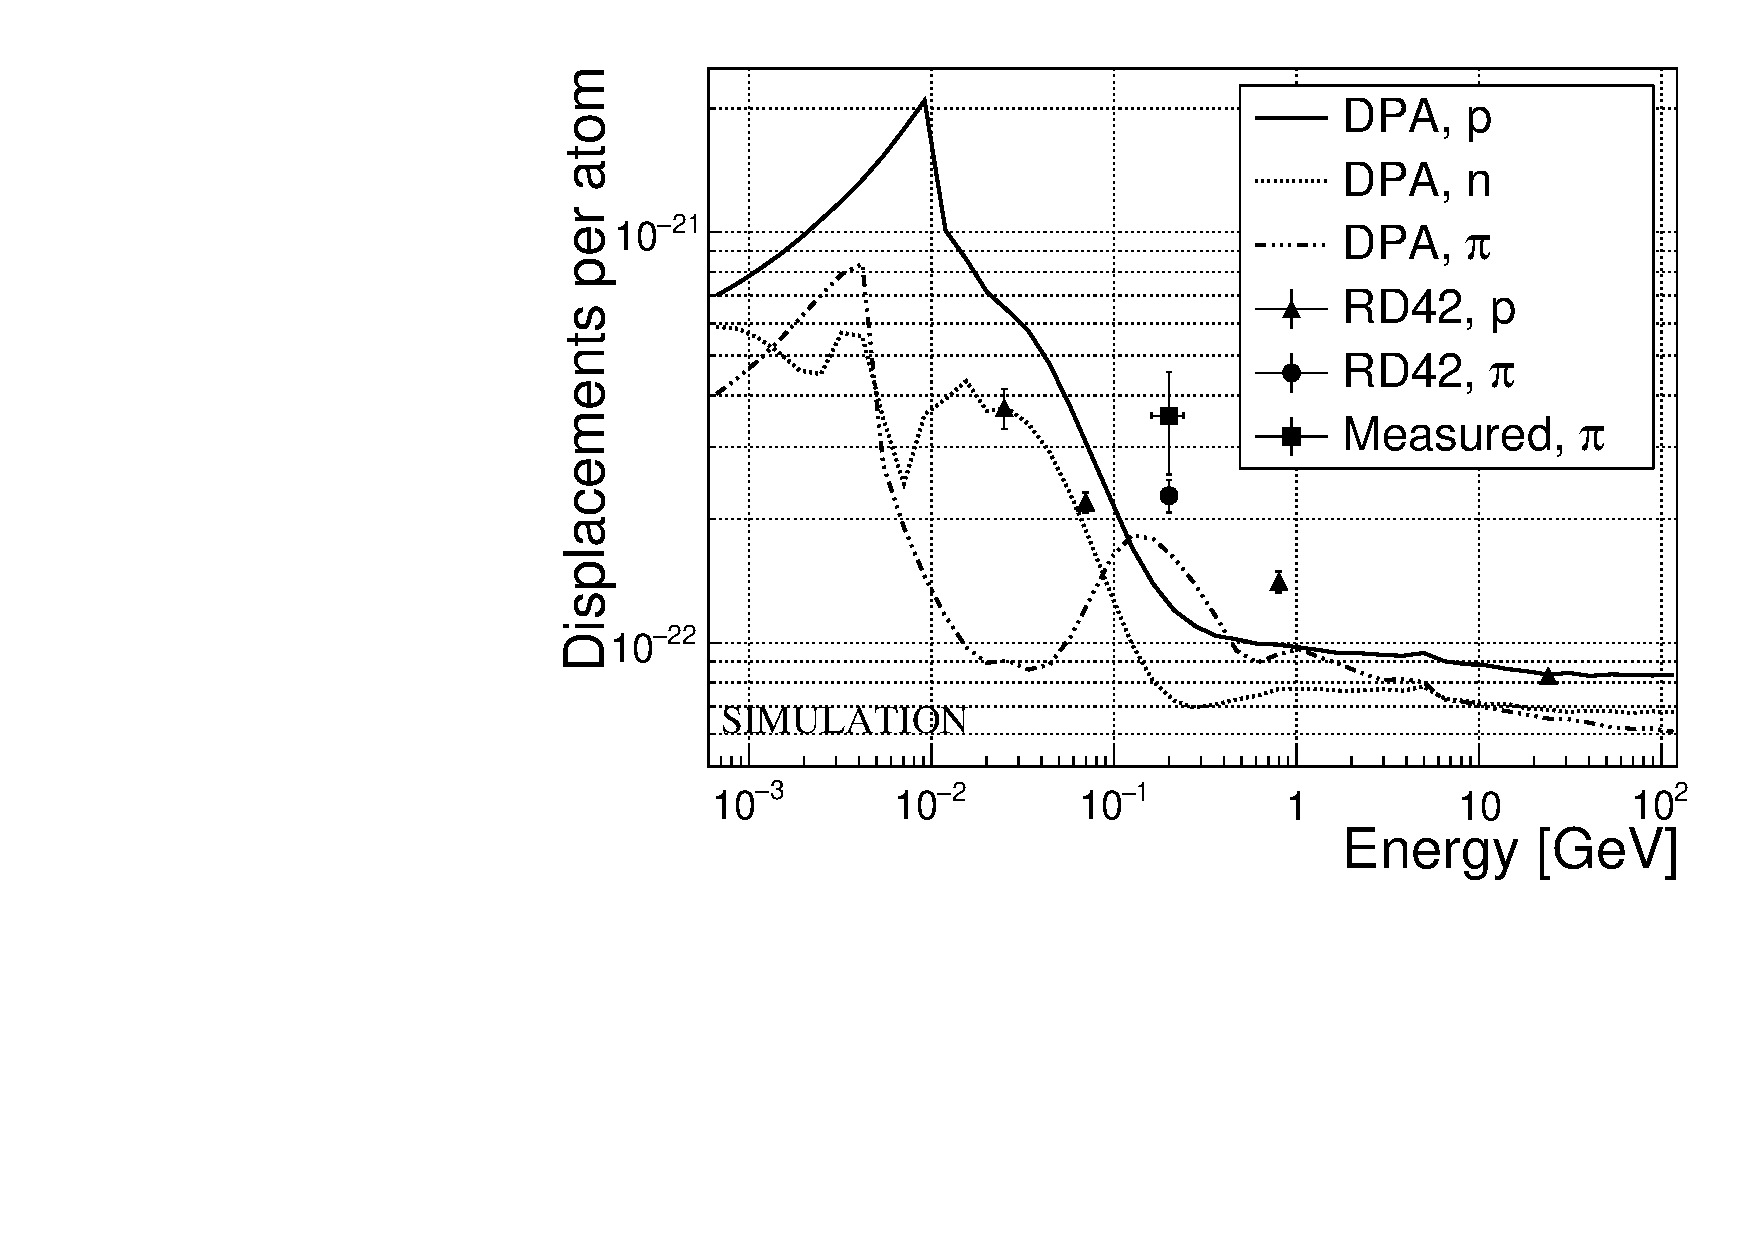
\includegraphics[width=0.8\textwidth]{03_measurement_results/scripts/plots/dpa1}
\caption{Diamond radiation damage - a model based on displacements per atom~\cite{Guthoff:2014223}. Added are data points for protons and pions by RD42~\cite{RD42IRRAD:00000} and one data point for pions measured in the scope of this thesis.}
\label{fig:kitdpa}
\end{center}
\end{figure}



\subsubsection{Irradiation with a $\uppi_\mathrm{300~MeV}$  beam}
The samples were irradiated at the Paul Scherrer Institute (PSI)~\cite{PSI:00000} by means of a beam of pions with an energy of 300~MeV (kinetic energy 191.31~MeV) and with a flux of up to $1.5\times10^{14}~\pi$~cm$^{-2}$ per day. The system has a 10~\% uncertainty on the beam energy. In addition, their quoted uncertainty on the measurement has an error of $\pm20~\%$. Looking at the pion damage curve in figure~\ref{fig:kitdpa}, $\pi_{\mathrm{300~MeV}}$ point sits on a steep section of the DPA curve. This means that a deviation in beam energy can have a significant effect on the damage.
%After fitting a linear function between, the error on the DPA due to the uncertainty on the beam energy amounts to 7~\%. Overall error on the fluency is therefore the root mean square of the uncertainty on the DPA and the uncertainty on the hardness factor: $\upsigma=21~\%$.

Two diamond samples, S52 and S79, were put in the $\uppi_\mathrm{300~MeV}$ beam in the 2014 PSI irradiation campaign; S52 to $(1\pm0.21)\times10^{14}~\pi$~cm$^{-2}$ and S79 to $(3.63\pm0.77)\times10^{14}~\pi$~cm$^{-2}$. During the process, the golden electrodes got slightly activated, but the activation decayed in two weeks.

\subsubsection{Charge collection efficiency and charge collection distance}
Three diamonds -- non-irradiated S37 and irradiated S52 and S79 -- were tested in a $\uppi_\mathrm{120~GeV}$ test beam in the SPS North Experimental Area at CERN~\cite{Brianti:604383} before and after irradiation. The goal was to estimate the charge collection efficiency (CCE) and charge collection distance (CCD) as a function of irradiation dose. The samples were primed (pumped) prior to data taking using a $^{90}$Sr radioactive source. The data were then taken at a range of bias voltages ranging from 30~V to 900~V, yielding between 0.06~V/$\upmu$m and 1.8~V/$\upmu$m electrical field in the bulk. Every data point contained approximately $5\times10^4$ measured particles. The charge deposited by the particles was measured using a CIVIDEC Cx charge preamplifier. As expected, the integrated amplitude spectrum followed a landau distribution.
%, as seen in figure~\ref{fig:landausample}. 
Its most probable value (MPV) was used to calculate the most probable collected charge $Q_\mathrm{i}$:
\begin{equation}
\label{eq:ccdcalc}
Q_\mathrm{i}~[e^-] = \frac{ Q_i~[fC] } { 1.6\times 10^{-4} }= \frac{MPV~[mV]}{A~[mV/fC]} \cdot 6.241\times 10^{4}
\end{equation} 
where A$=9.2$~mV/fC is the preamplifier gain factor. The CCD was then calculated using the average number of electron-hole pairs produced per micrometer in diamond $\delta_d = 36~$e-h~$\upmu$m$^{-1}$ (from table~\ref{tab:semicompare}):
\begin{equation}
\label{eq:ccdcalc1}
CCD = \frac{Q_\mathrm{i}}{\delta_\mathrm{}d}
\end{equation} 

% sample landau distribution  
%\begin{figure}[!t]
%\begin{center}
%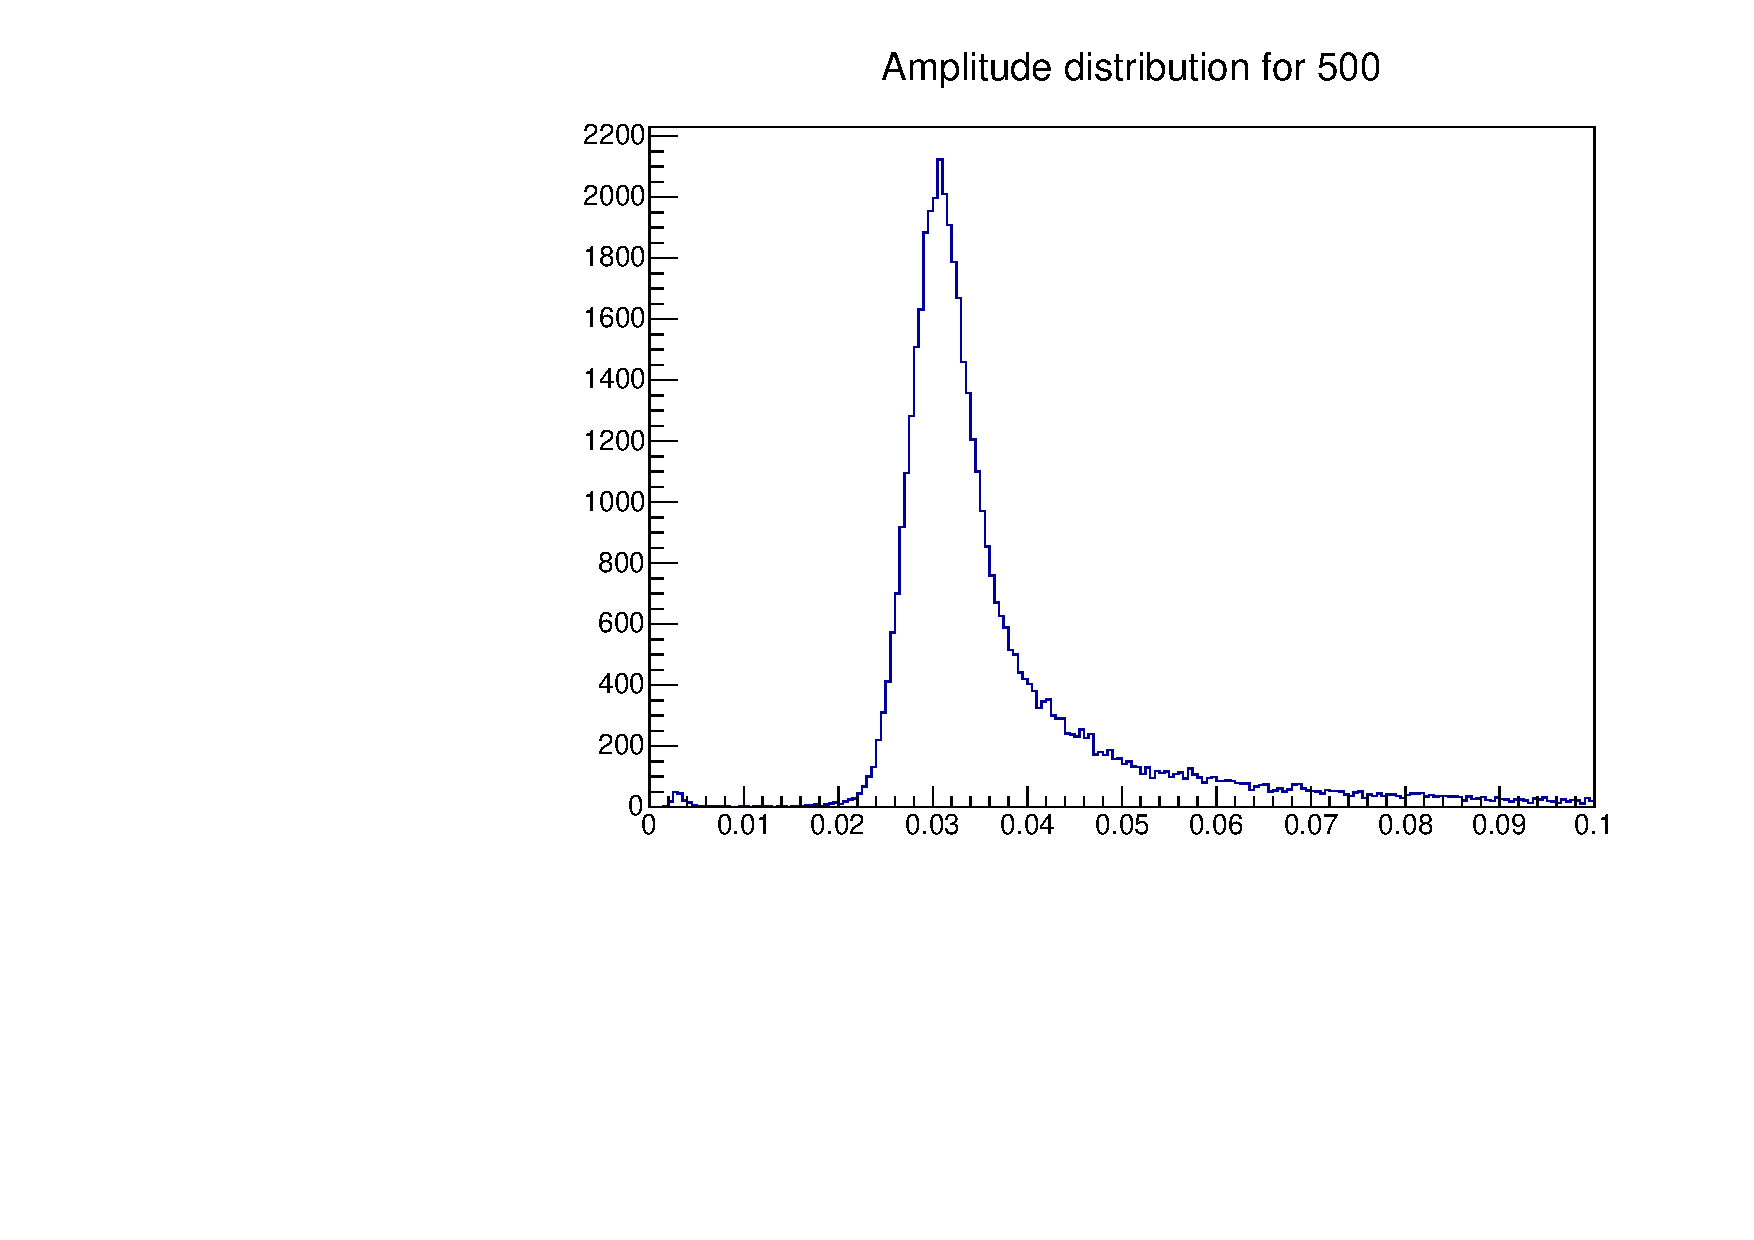
\includegraphics[width=0.6\textwidth]{03_measurement_results/scripts/pics/S37_500}
%\caption{An example of a landau distribution acquired by S37 at 500~V bias voltage PLACEHOLDER}
%\label{fig:landausample}
%\end{center}
%\end{figure}
The resulting CCD for the three measured samples at bias voltages ranging from 0.2--1.6~V~$\upmu$m$^{-1}$ is shown in figure~\ref{fig:ccd}. S37 exhibits a full collection distance already at 0.4~V~$\upmu$m$^{-1}$ whereas the irradiated samples have a more gentle increase of CCD with increasing bias voltage. It is evident that at 1~V~$\upmu$m$^{-1}$  the maximum CCD has not been reached in the case of S79 and S52. Nevertheless, to compare the measured data point with those provided by RD42, the CCD at 1~$\upmu$m has to be taken.

% CCD against HV 
\begin{figure}[!t]
\centering
\begin{tabular}{cccc}
\subfloat{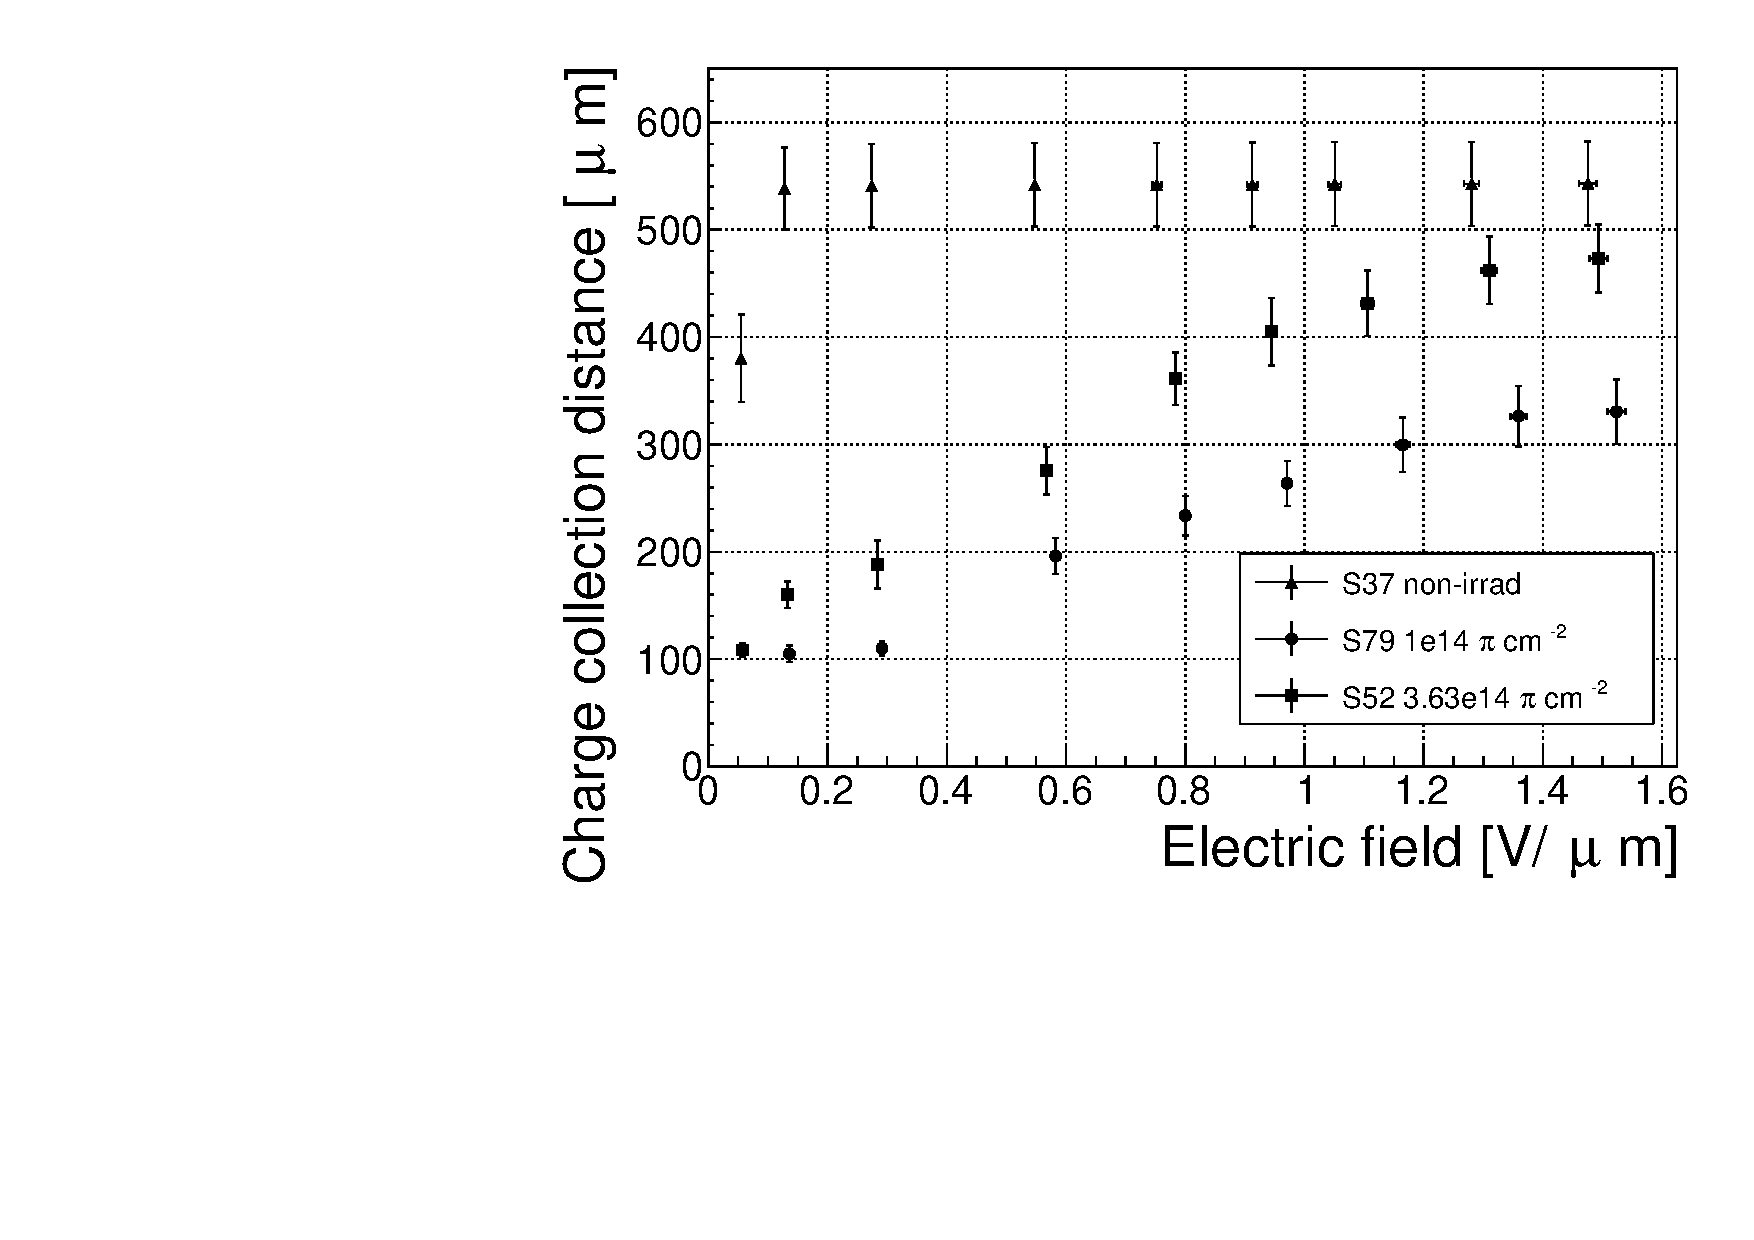
\includegraphics[width=0.80\textwidth]{03_measurement_results/scripts/plots/ccd} \label{fig:ccd}} \\
\subfloat{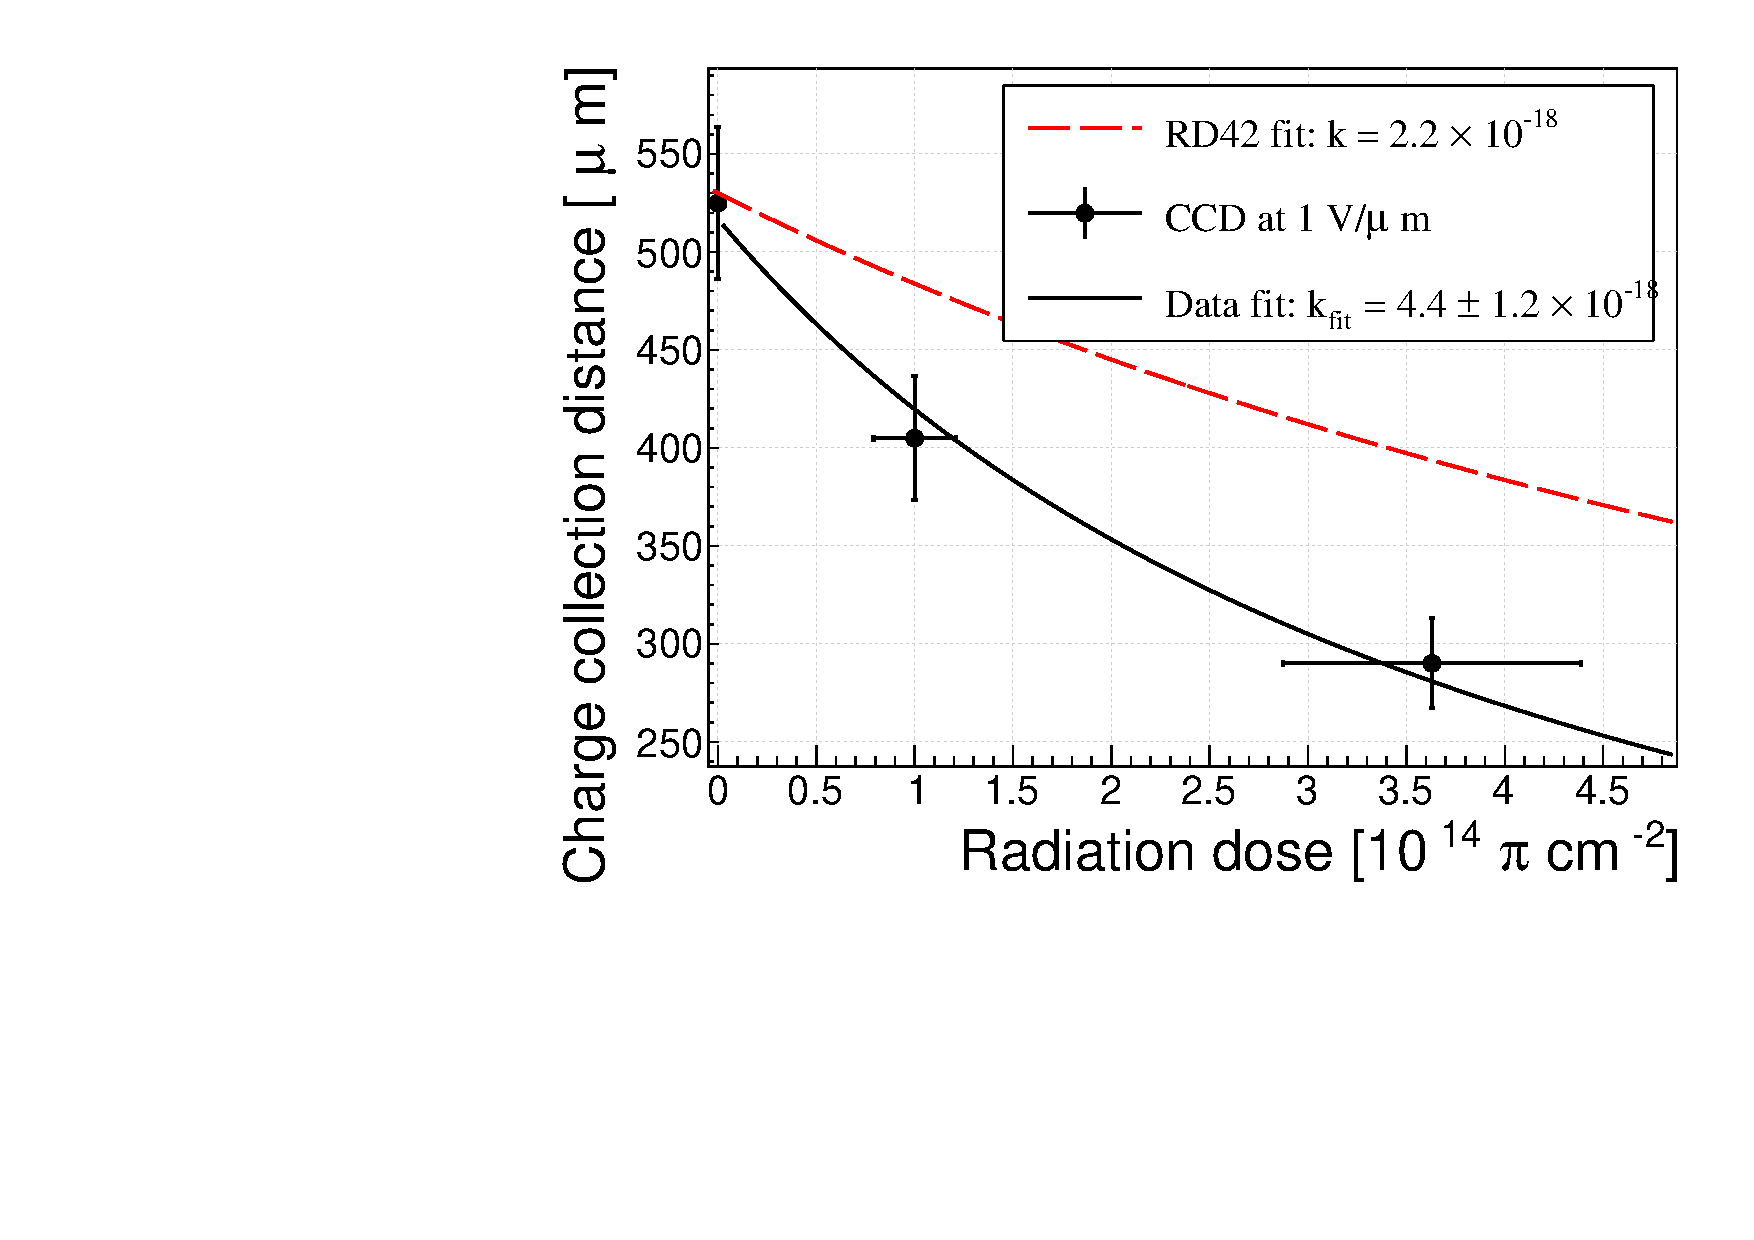
\includegraphics[width=0.80\textwidth]{03_measurement_results/scripts/plots/radfactor1}  \label{fig:radfactor}}
\end{tabular}
\caption{First figure shows the CCD for S37, S79 and S52 at a range of bias voltage settings. The charge collection distance at 1~V/$\upmu$m bias voltage for the three diamond samples is then compared to the RD42 data for pion irradiation in the second figure. The data points are about 15--25~\% lower than expected from the RD42 data~\cite{RD42IRRAD:00000}.}
\end{figure}

\subsubsection{Irradiation damage factor}
The irradiation damage factor $k$ is a way to quantify irradiation damage of a specific particle at a specific energy. Via this factor different types of irradiation can be compared. It is obtained experimentally by measuring the CCD of a number of samples at various irradiation steps and fitting the equation~\ref{eq:radfactor1} to the data. $\lambda$ is the measured CCD, $\lambda_\mathrm{0}$ is the CCD of a non-irradiated sample and $\Phi$ the radiation dose. As a reference, the damage factor for 24~GeV protons is set to $1\times10^{-18}~\upmu$m$^{-1}$~cm~$^{-2}$.


\begin{equation}
\label{eq:radfactor}
\frac{1}{\lambda} = \frac{1}{\lambda_\mathrm{0}}+k_{\lambda}\cdot\Phi
\end{equation} 
\begin{equation}
\label{eq:radfactor1}
\lambda = \frac{\lambda_\mathrm{0}}{k_{\lambda} \lambda_0 \Phi + 1}
\end{equation} 

The data points with the maximum CCD obtained in the test beam measurements are plotted against radiation dose received (see figure~\ref{fig:radfactor}). Equation~\ref{eq:radfactor1} is fitted to the data points and a damage factor $k_{\mathrm{\lambda}}=(4.4\pm1.2)\times10^{-18}~\upmu$m$^{-1}$~cm~$^{-2}$ was obtained. This value is for a factor of two higher than the damage factor obtained by RD42. %The irradiated samples do not yet have a full charge collection at 1.0~V~$\upmu$m$^{-1}$. 
This could be due to an insufficient priming time ahead of the measurement. In addition, the diamond samples have not been polished and re-metallised after irradiation, as is the case for the RD42. Also, with only two samples measured, the statistical uncertainty is high. Nevertheless, it can be concluded that the 300~MeV pions damage the diamond bulk more than the 24~GeV protons.




\subsection{Long-term measurement stability}
An important requirement for particle detectors is a stable performance over long periods of time. For instance, the charge collection for a defined radiation type and quantity must not change over time or has to change in a predicted way. Diamonds are stable as long as their environment and their operating point does not change significantly. The stability of diamond detectors depends on many factors (material purity, polishing process, electrode material, irradiation damage etc.). The aim is to study the behaviour of diamond under controlled conditions, with the goal to understand its limitations. One of these limitations is for sure the received radiation dose as it can affect the long-term stability of the sensor during operation. 

The three diamond samples (S37, S79 and S52) have been exposed to two different types of ionising radiation for a longer period to see if their behaviour changes over time. Two parameters have been observed in particular: 
\begin{enumerate}
\item Charge collection of $\upbeta$ particles and 
\item Charge collection and ionisation profile of $\upalpha$ particles.
\end{enumerate}
The results in this and in the next section will show that, in both cases, priming plays an important role in improving the diamond measurement stability. 
%NOTE I can use this part for conclusion
%The $\upbeta$ particles have a ``healing'' effect on the diamond; MIP detection is therefore rather stable in the long run, despite the fact that the sensors had been degraded by means of irradiation. Alpha particles, on the other hand, deteriorate the measurement, probably by introducing space charge into the sensor bulk. 

\subsubsection{$\upbeta$ long-term stability}
The diamond samples have undergone a long-term stability test using $\upbeta$ radiation. This has been done using a $^{90}$Sr source emitting $\sim$2~MeV electrons at a rate of approximately $10^4$~e$^-$~cm$^{-2}$. To simulate the initial conditions in HEP experiments, the sensors must not be primed before starting the measurements. The measurement setup consists of a diamond sample (S37, S52 or S79) with the Cx spectroscopic amplifier, a silicon diode with a C6 amplifier for a trigger and a $^{90}$Sr source on top. A particle emitted by the source traverses the sensor bulk and hits the silicon diode, triggering the analogue signal readout. The source is left on the top for the course of the experiment. The measurements, however, are taken at discrete times. For every data point, approximately $10^4$ triggers are recorded. The offline analysis of the recorded signal pulse amplitudes yields a landau distribution for every data point. The most probable value (MPV) of the distribution is proportional to the collected charge by the diamond sensor. The resulting graph of charge collection over time (see figure~\ref{fig:ccincrease}) shows that the charge collection efficiency improves when the diamond sensor is primed with a $\upbeta$ source. This is especially evident in the case of the two irradiated samples. S79 achieves close to a full efficiency whereas S52 reaches about 50~\%. Both increases are significant. At a received dose of approximately 4$\times10^6$~particles the signal stabilises. As expected, the signal of the non-irradiated S37 does not change with time -- this pure sCVD diamond sample has the maximum collection distance from the start of the measurement.

It should be noted that the $\sim$2.28~MeV electrons emitted by this source are not MIPs; their charge deposition is higher than that of an electron MIP, according to the Bethe-Bloch distribution~\cite{BETHE:00000}. Nevertheless, for the purpose of these measurements this energy was adequate since only the relative change in charge collection was of our interest.

To sum up, diamond is a good choice for $\upbeta$ radiation detection. Even if damaged by radiation, it reaches a stable charge collection at a received dose of $\sim$4$\times10^6$~MIP particles. The efficiency decreases with a high irradiation dose (effects visible above 10$^{12}$~MIP~cm$^{-2}$). However, the decrease can be accounted for if the damage factor and the rate and energy of the particles are known. $\upgamma$ radiation has a similar impact on the diamond as the $\upbeta$ because the ionisation mechanism is the same. The incident photons, if they interact with the diamond, prime the bulk, causing the increase in charge collection efficiency. The difference, however, is that the interaction probability (cross section) is lower for gammas~\cite{sarin2014comprehensive,Griesmayer20121997}.

%%longterm pumping plot
\begin{figure}[!t]
\begin{center}
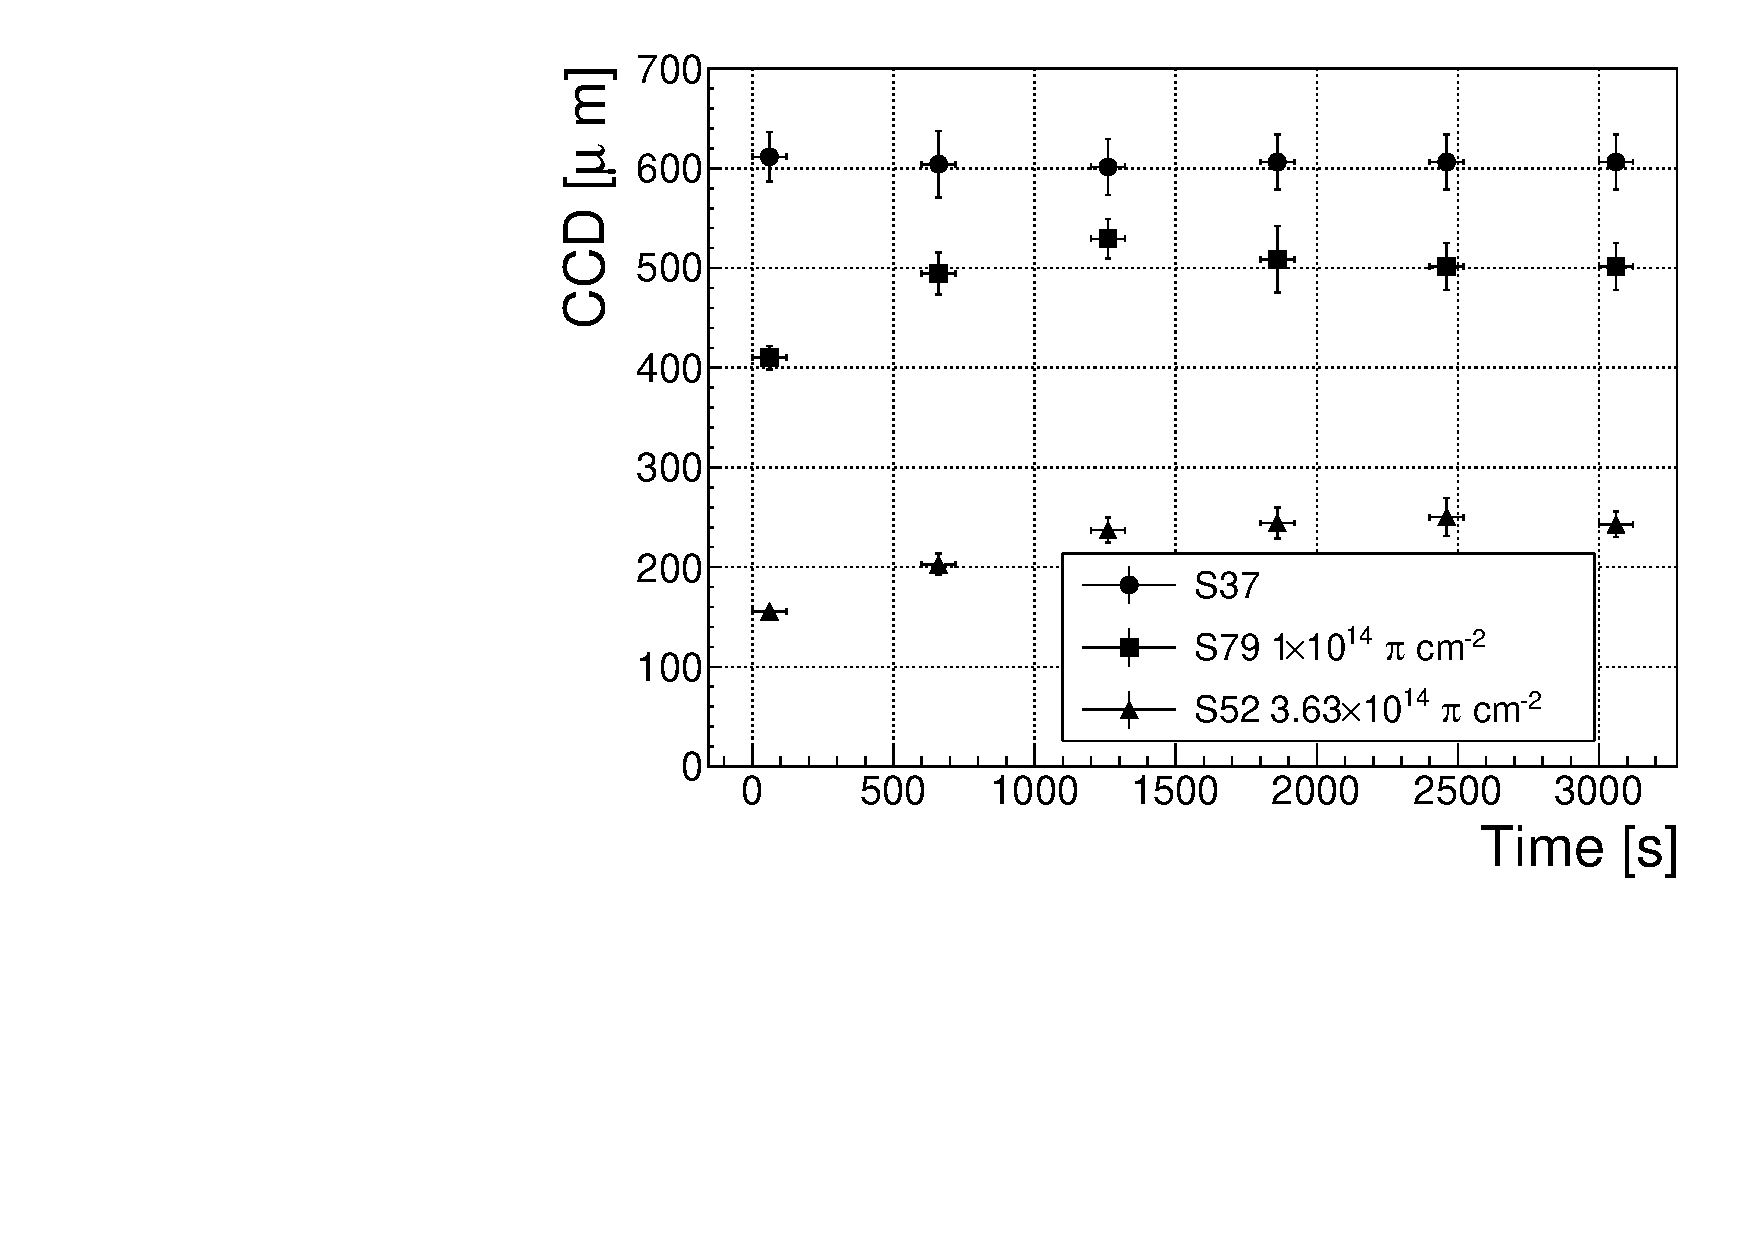
\includegraphics[width=0.8\textwidth]{03_measurement_results/plots/ccdpriming}
\caption{Relative increase of charge collection over time due to priming with the $^{90}$Sr radioactive source. The charge collection for the non-irradiated S37 stays constant. The bias voltage for this measurement is 1~V/$\upmu$m.}
\label{fig:ccincrease}
\end{center}
\end{figure}


\subsubsection{$\upalpha$ long-term stability}
This part discusses the stability of irradiated diamond sensors during $\upalpha$ measurements. An $^{241}$Am source is used, emitting $\upalpha$ particles with a mean energy of 5.5~MeV. It is safe to assume that they will behave differently than when subject to $\beta$ radiation. This is due to the point-like charge carrier creation when an $\upalpha$ particle penetrates the bulk and stops at a depth of $\sim$14~$\upmu$m (for a 5.5~MeV particle). The deposited energy produces $\frac{5.5~MeV}{13.6~eV} = 4\times10^5$ e-h pairs. Compared to a MIP, which produces an MPV of $500~\upmu m~\times~36~e-h~\upmu m^{-1} = 18\times10^3$ e-h pairs in a 500~$\upmu$m, the collected charge is for a factor of 22 higher. In addition, the energy is deposited in a small volume -- 14~$\upmu$m in depth and $\sim$20~nm radially~\cite{Jansen:1956431}. This dense distribution of charge carriers affects their behaviour at the start of the drift. Furthermore, carriers of only one polarity drift through the sensor while those of the opposite polarity almost instantly recombine with the adjacent electrode. Taking into account that the diamond bulk has been damaged by irradiation, these two phenomena might have an effect on the operation of the detector on a macro scale.

%The measurement setup consisted of a PCB carrier for a diamond with a fitted $^{241}$Am source and a vacuum chamber. The carrier was placed into the chamber, which was then evacuated. t acted as shielding for external noise pickup and ensured that the $\upalpha$ particles didn't lose energy traveling through air. An SMA feedthrough ensured the electrical connection to the outside. The samples were measured before and after priming, at both polarities, to compare the behaviour of both electrons and holes as charge carriers. The scope of the measurements was to observe the changes in charge collection efficiency and/or in the pulse shapes. 

The first test has been carried out using the Cx spectroscopic amplifier, with the bias voltage of the samples set to +500~V. Figure~\ref{fig:longtermcx} shows the results of 6500 recorded hits at a rate of $\sim$7~particles per second. The collected charge $Q(\Phi)$ for the non-irradiated sample is stable as compared to the initial collected charge $Q(0)$ (plotted as a relative value $\frac{Q(\Phi)}{Q(0)}$). It is expected that the irradiated samples will have a lower charge collection efficiency than the non-irradiated sample. However, their initial efficiency suddenly drops after a certain period of time. The initial efficiency after priming with $\upbeta$ particles is higher than that without priming, but eventually it deteriorates again. In addition, the spread of measured energies increases significantly. Finally, the particle counting rate decreases with the decreased efficiency. 
\begin{figure}[!t]
\begin{center}
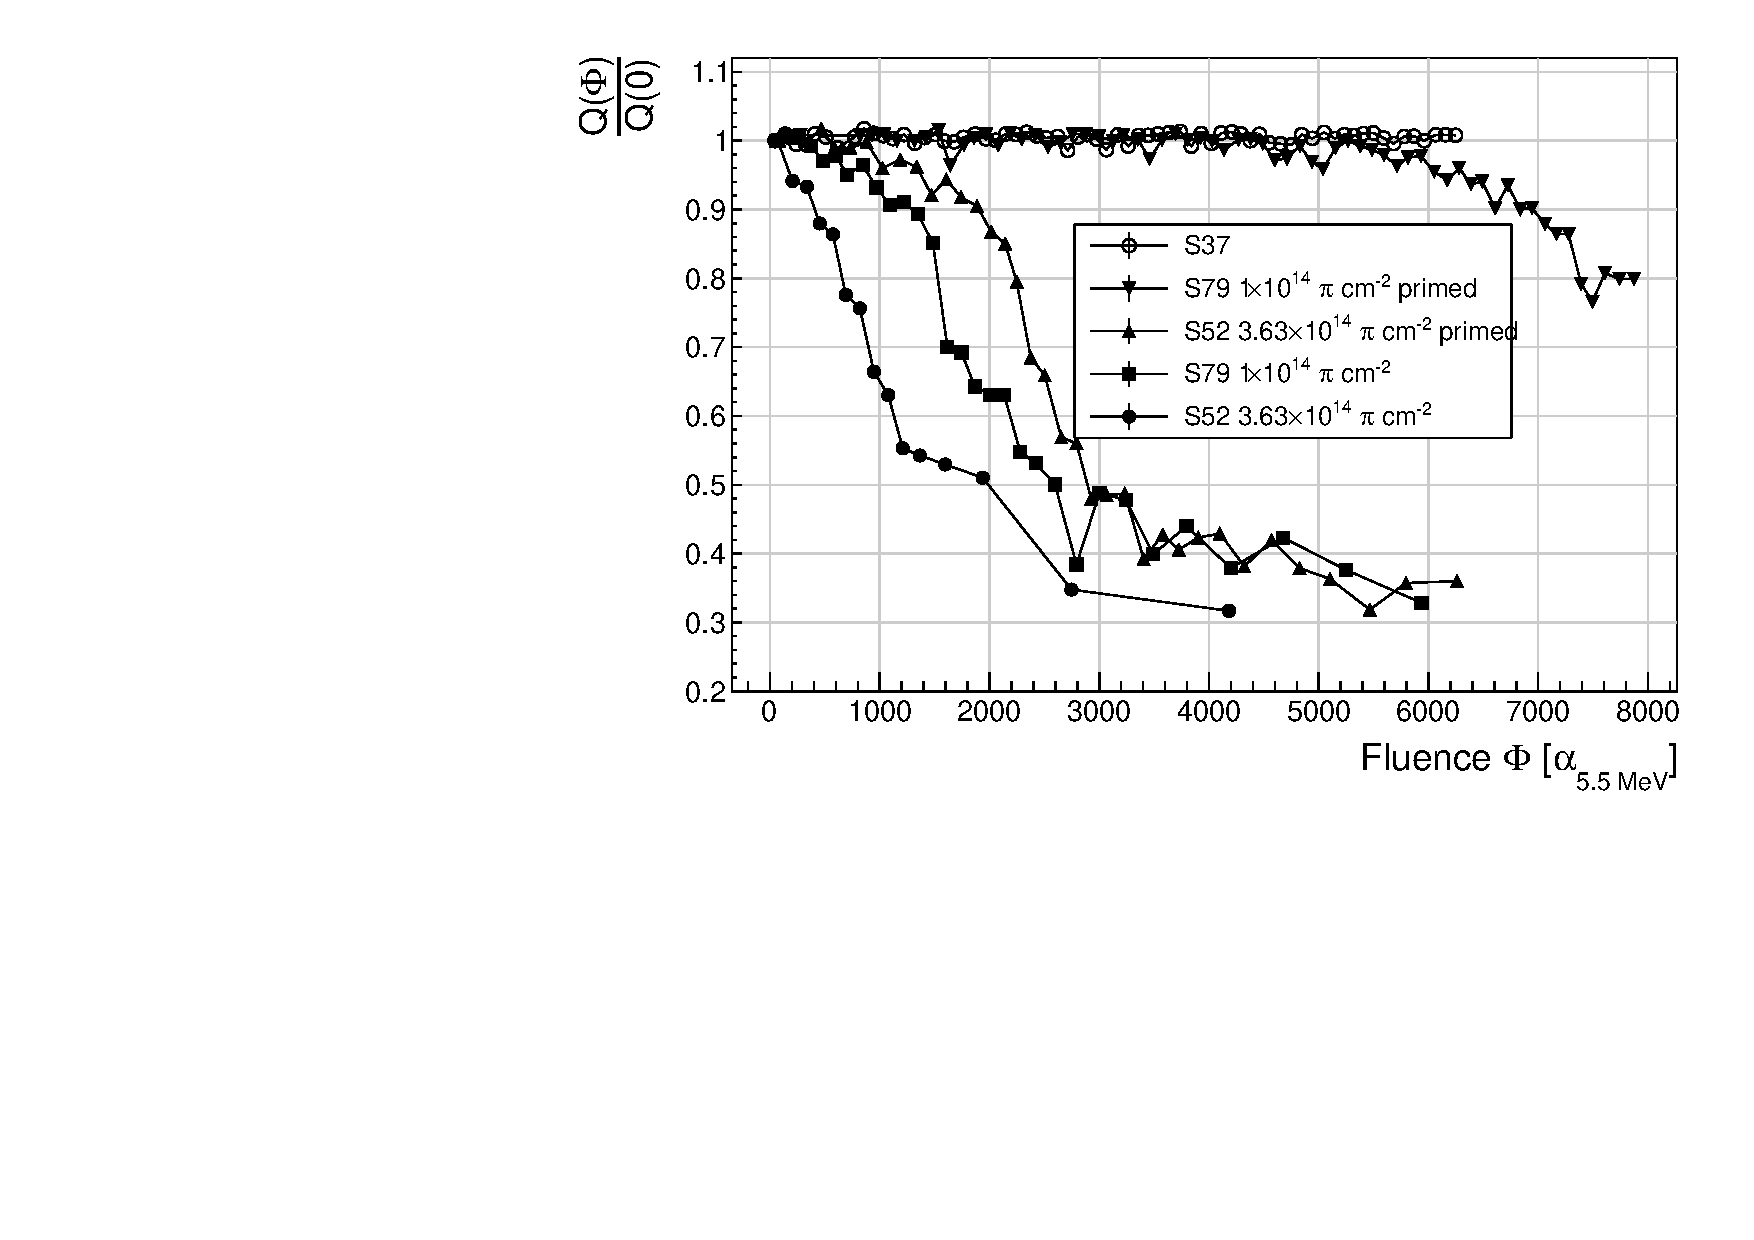
\includegraphics[width=0.8\textwidth]{03_measurement_results/scripts/plots/amplvstimecx4}
\caption{Relative decrease of collected charge with time for non-irradiated and irradiated diamond samples.}
\label{fig:longtermcx}
\end{center}
\end{figure}

To investigate this sudden drop in efficiency, the current pulse shapes using a C2 current amplifier have to be observed (see figure~\ref{fig:lifetimeelecsholes}). The shape of the pulse holds more information about the charge carrier properties in the sensor than solely the value of the integrated charge. This time only the primed S79 sample has been tested. Both hole and electron collection are observed to determine whether they behave differently or not. The sample has been measured long enough for the pulse shapes to start changing. The data in figures~\ref{fig:lifetimeelecsholes} show that the initially stable pulses start deteriorating -- suddenly several different shapes start appearing, some still very similar to those from the beginning while the others with almost zero amplitude. 

Some charges get stopped in the charge traps in the bulk for a long time, building up regions of space charge. 
%DISCUSSION!!!
%Since only one charge flavour is drifting through the bulk whereas the other is quickly recombined, this already determines the imbalance in spatial distribution of trapped charges. 
The built up space charge affects the electric field, making it non-uniform. The non-uniform field in turn affects the drifting carriers, slowing them down or speeding them up, depending on the field gradient. Since the movement of the carriers is inducing  the electric current, the field gradient can be observed in the signal. 

\begin{figure}[!t]
\centering
\begin{tabular}{rrr}
\subfloat{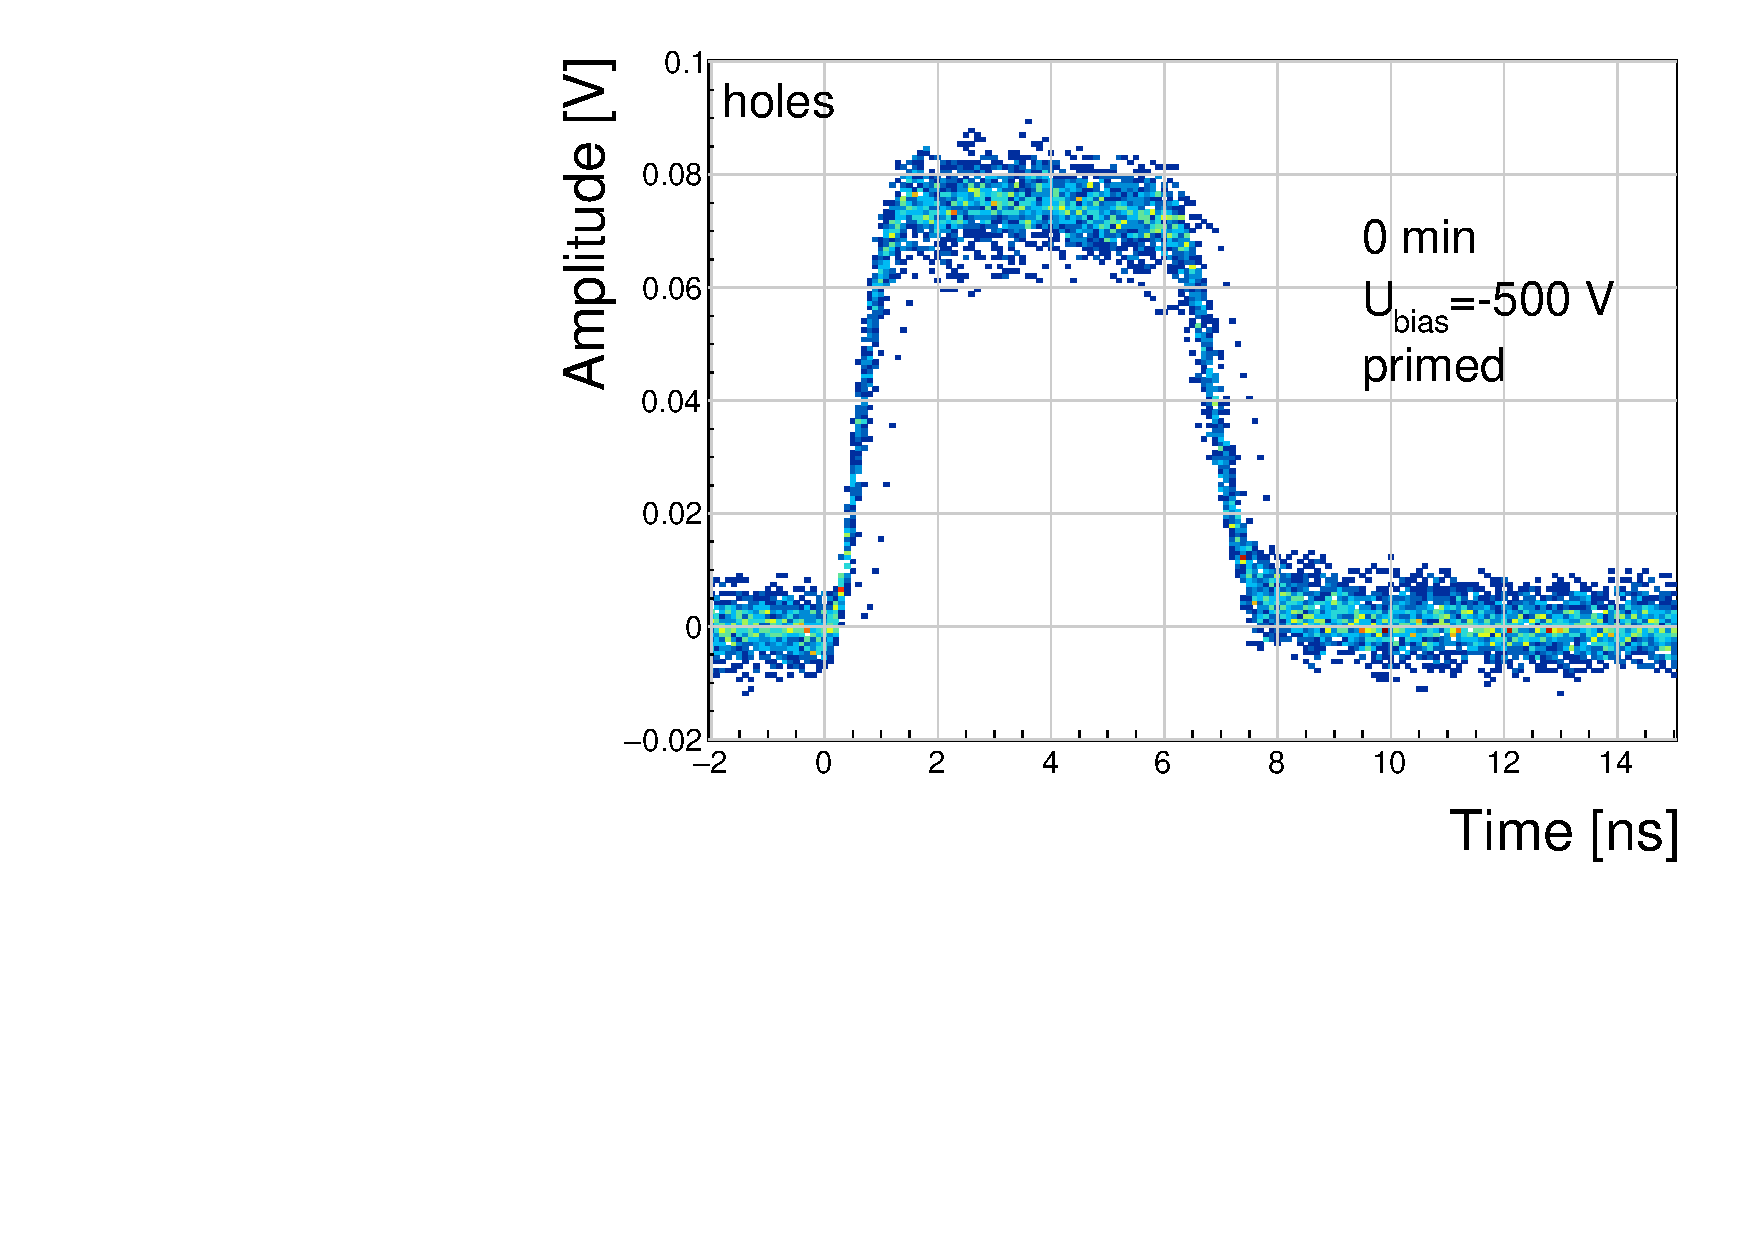
\includegraphics[width=0.47\textwidth]{03_measurement_results/scripts/plots/plotLifetime/holes0} \label{fig:holes0lt}} &
\subfloat{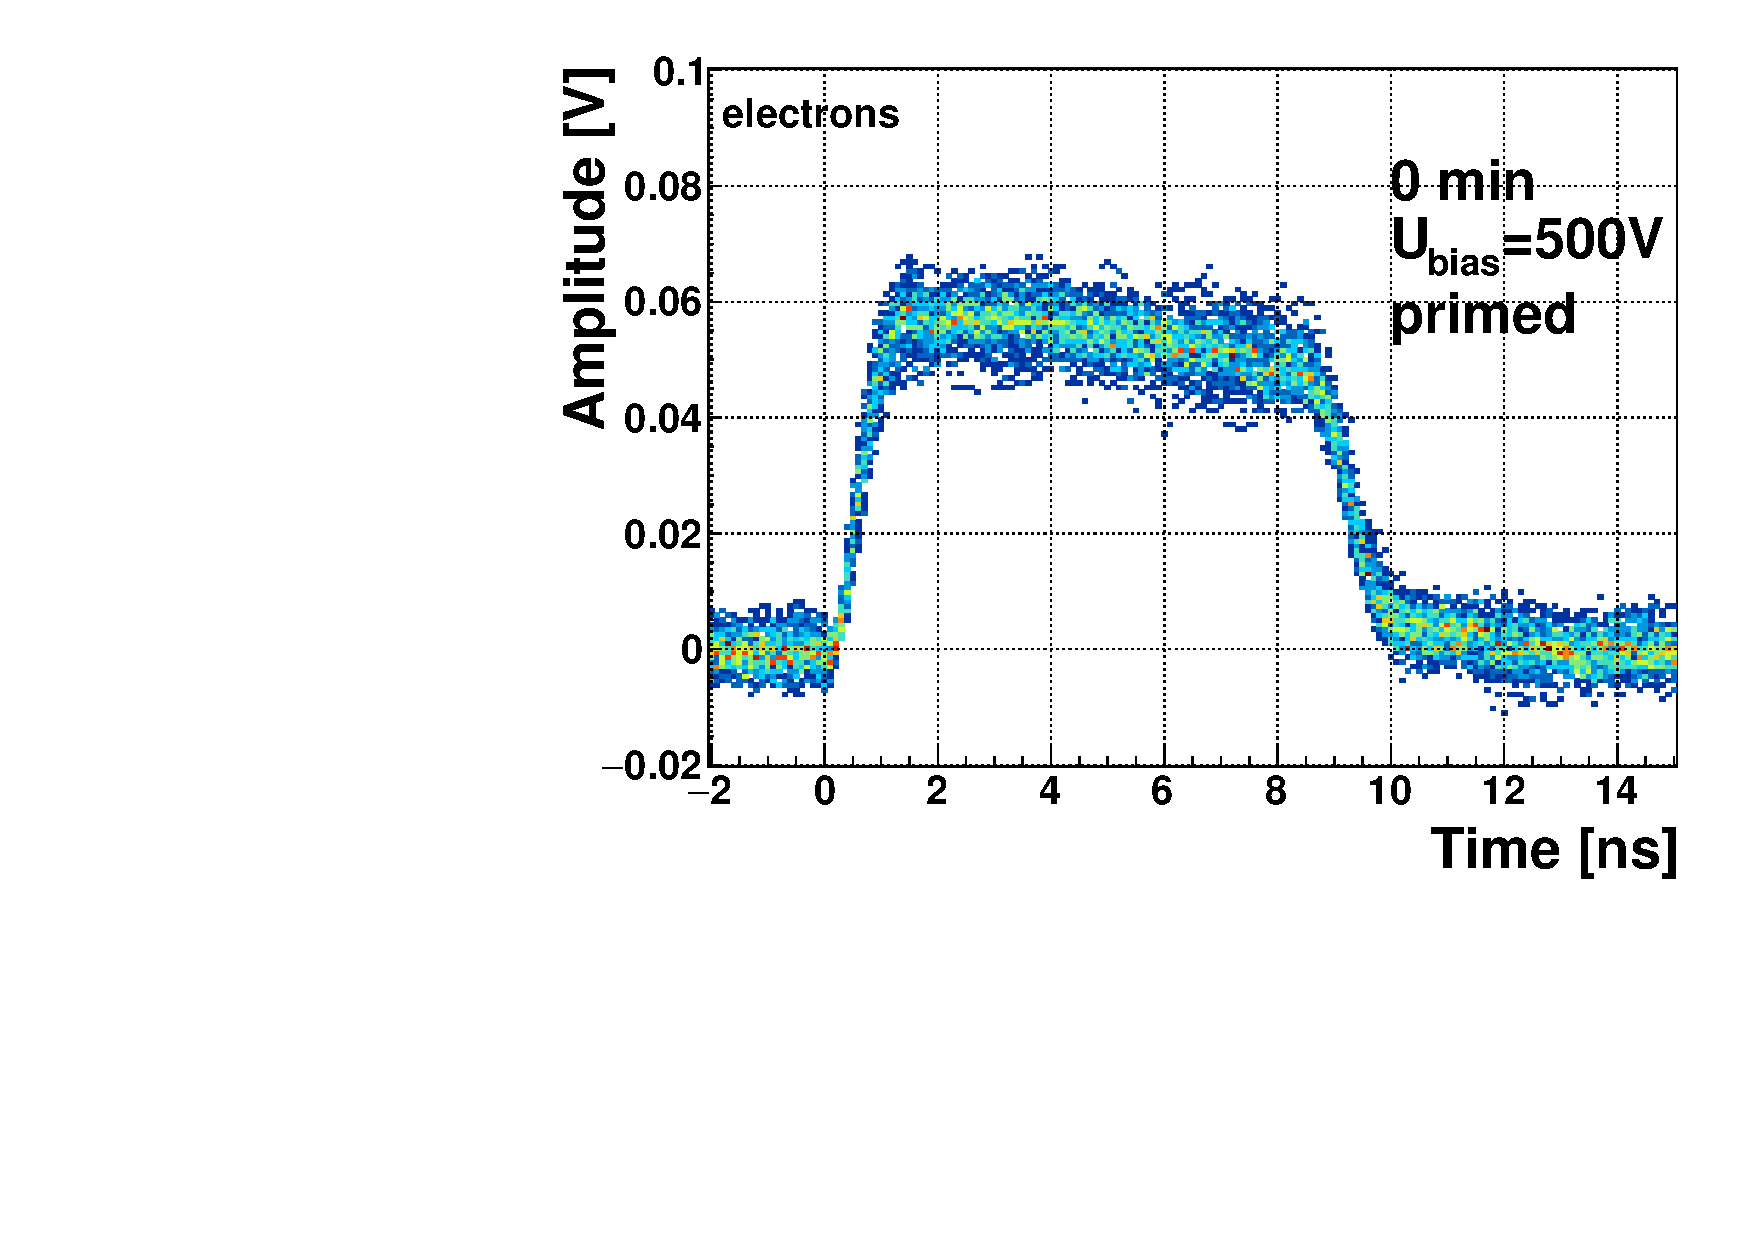
\includegraphics[width=0.47\textwidth]{03_measurement_results/scripts/plots/plotLifetime/elecs0} \label{fig:elecs0lt}} \\
\subfloat{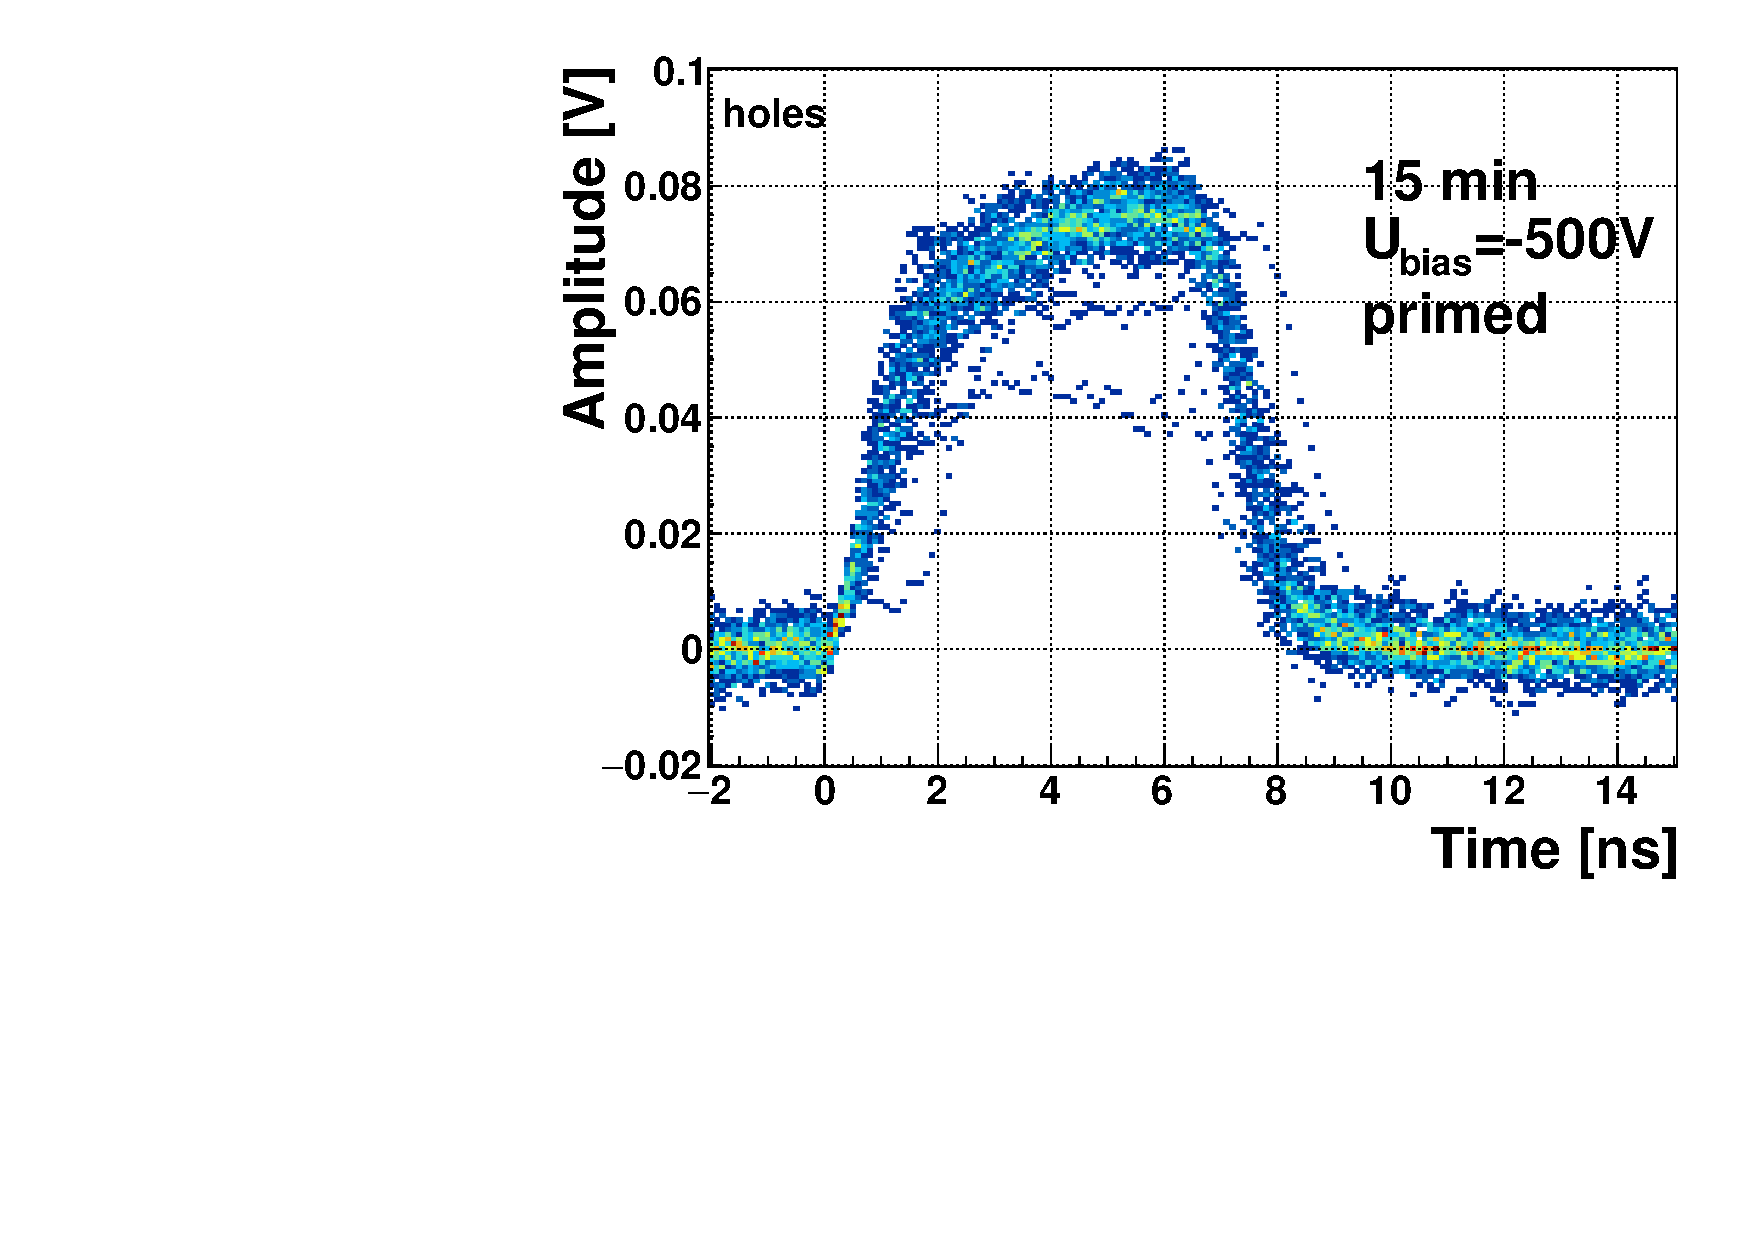
\includegraphics[width=0.47\textwidth]{03_measurement_results/scripts/plots/plotLifetime/holes15}  \label{fig:holes15lt}} &
\subfloat{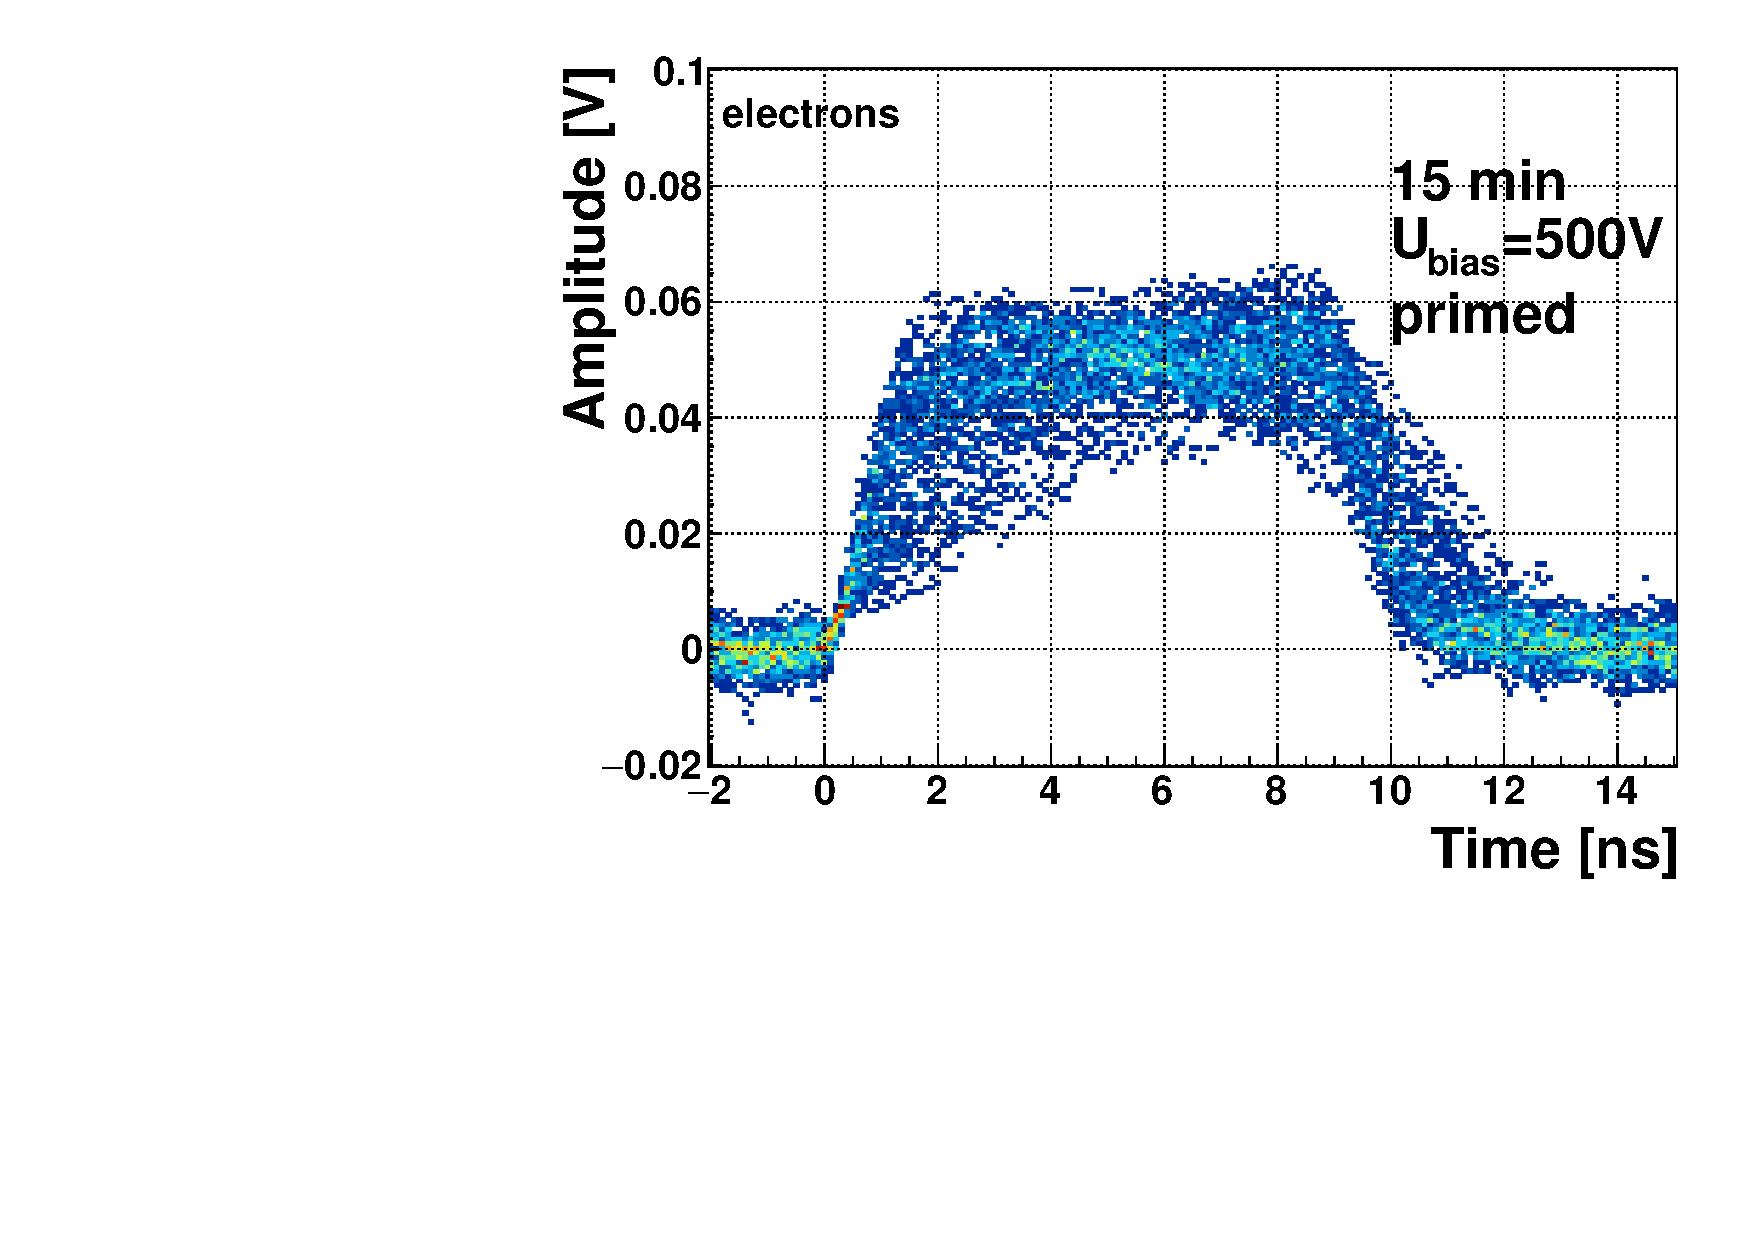
\includegraphics[width=0.47\textwidth]{03_measurement_results/scripts/plots/plotLifetime/elecs15}  \label{fig:elecs15lt}} \\
\subfloat{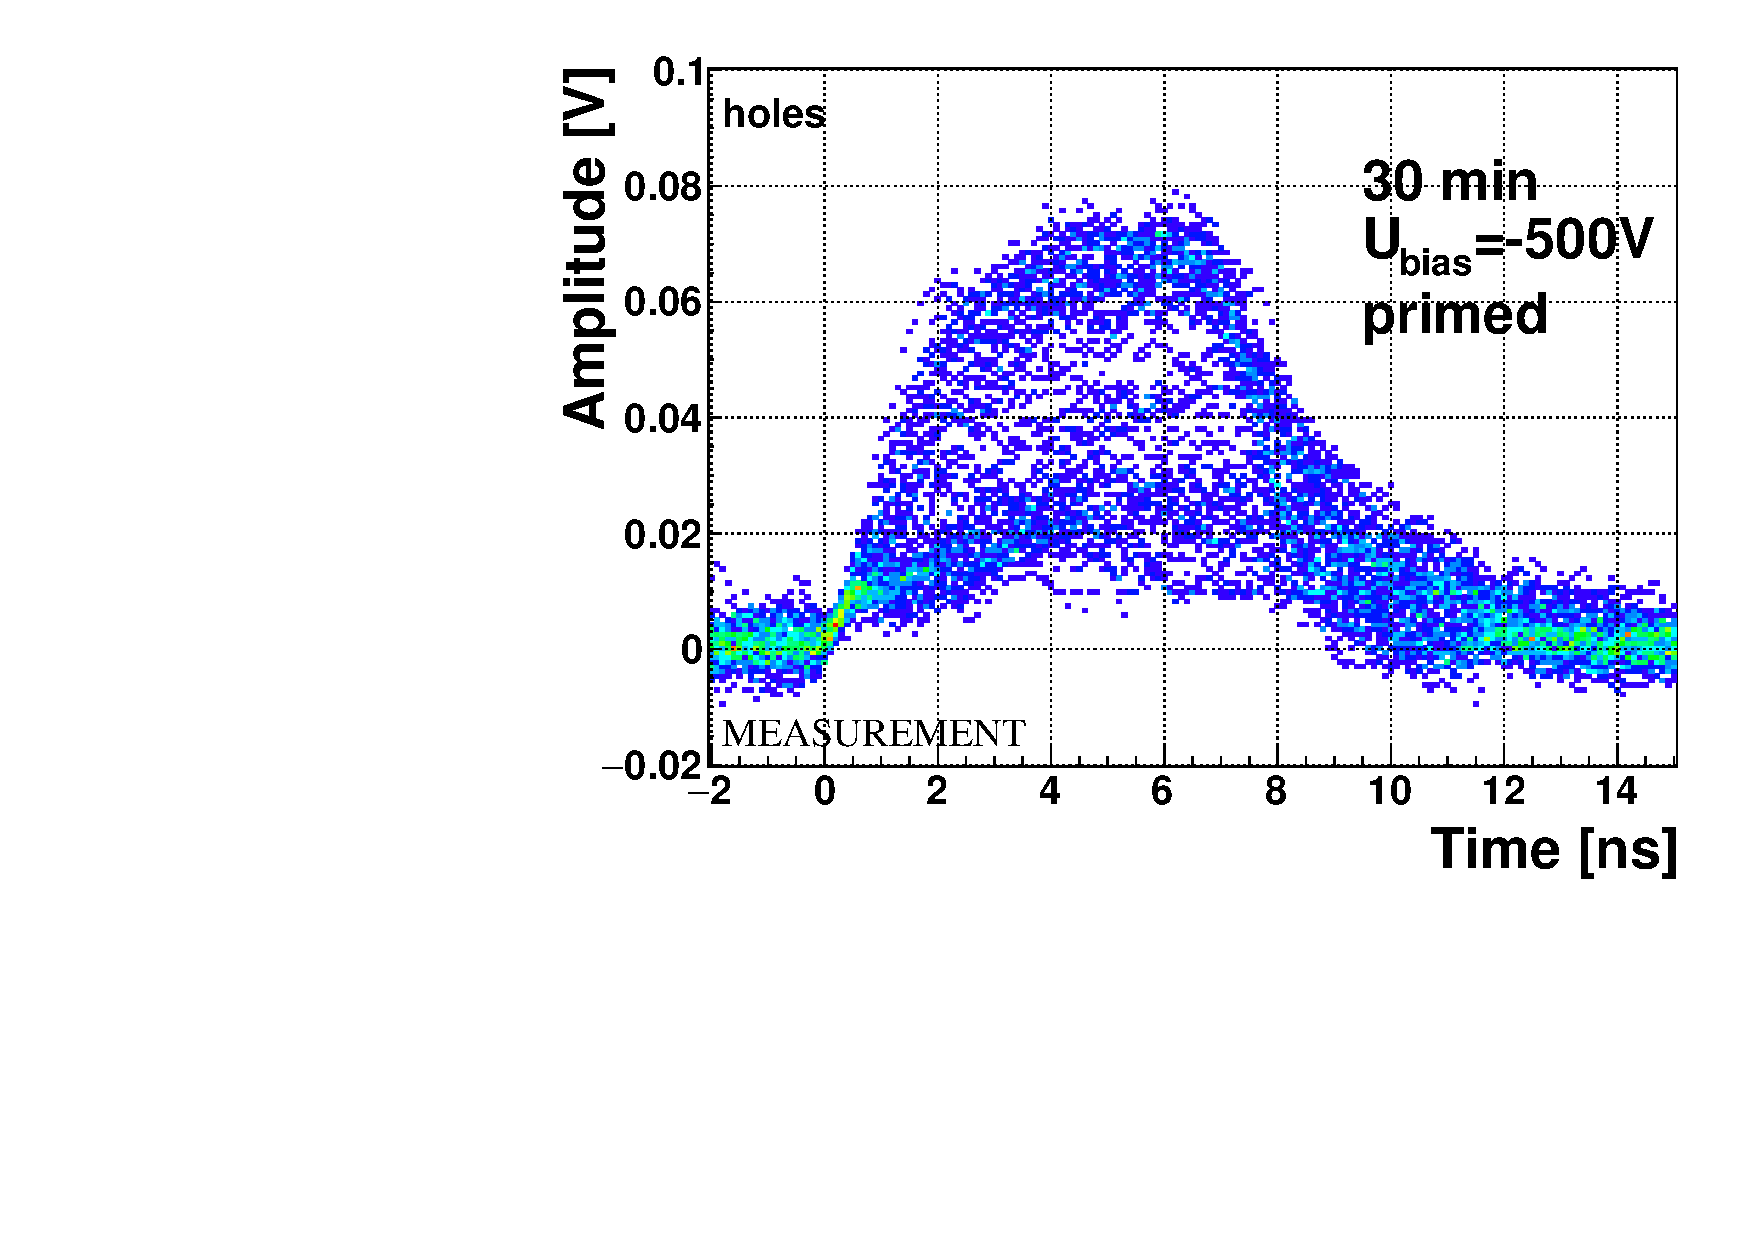
\includegraphics[width=0.47\textwidth]{03_measurement_results/scripts/plots/plotLifetime/holes30}  \label{fig:holes30lt}} &
\subfloat{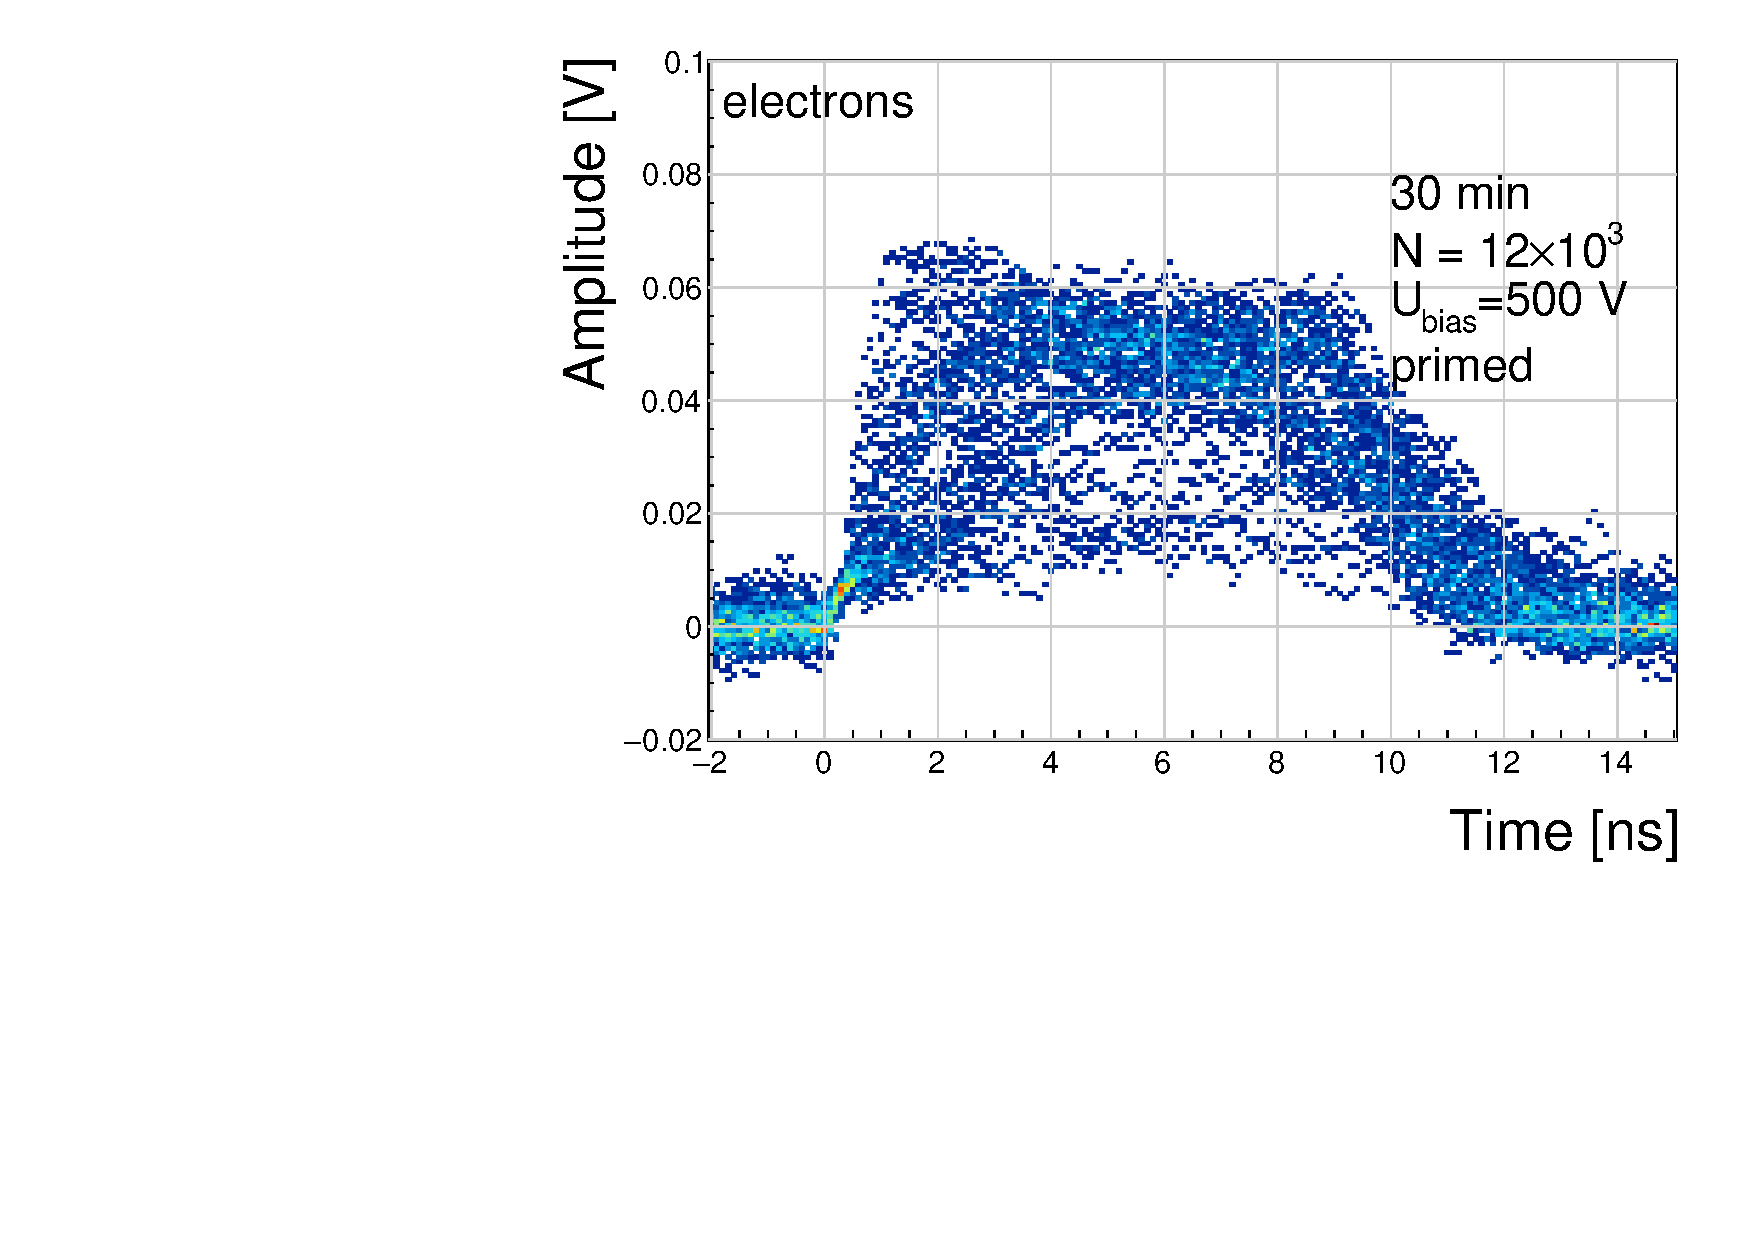
\includegraphics[width=0.47\textwidth]{03_measurement_results/scripts/plots/plotLifetime/elecs30}  \label{fig:elecs30lt}}
\end{tabular}
\caption{The signal of the irradiated and primed S79 deteriorates with time for both polarities. Every plot contains 60 superimposed pulses.}
\label{fig:lifetimeelecsholes}
\end{figure}

The second test with the C2 current amplifier has been carried out as follows: At the beginning of the test when the diamond is still operating stably, 60 pulses are recorded. An average pulse is calculated. This is a reference pulse for the subsequent measurement points.
% and plotted overlapped into a 2D histogram. An average pulse is extracted from this 2D distribution. 
Then an RMS of the single pulses with respect to the reference pulse is calculated and the values are summed together ($\sigma_\mathrm{ref}$). 

All the subsequent data points also consist of a set of 60 pulses. At every data point the summation of the RMS values of the individual pulses with respect to the initial averaged pulse is calculated ($\sigma$). The ratio between the initial $\sigma_{\mathrm{ref}}$ and discrete values $\sigma$ gives a measure of change of the pulse shape with respect to the reference pulse at the start of the measurement.
%, the shape correlation $Corr_{\mathrm{shape}}$ is calculated:
%\begin{equation}
%\label{eq:correlation}
%Corr_{\mathrm{shape}} (t) = \frac{\sigma_{\mathrm{ref}}}{\sigma} = \frac { \sum_\mathrm{x} \sum_\mathrm{y} w_{\mathrm{ref}}\cdot ( y_{\mathrm{avg}} - y_{\mathrm{ref}})^2 } { \sum_\mathrm{x} \sum_\mathrm{y} w\cdot ( y_{\mathrm{avg}} - y)^2 },
%\end{equation} 
%where $y_{\mathrm{avg}}$ is the amplitude of the current averaged pulse at time $x$, $y_{\mathrm{ref}}$ is the amplitude of the initial averaged pulse at time $x$, $y$ is the amplitude of the superimposed pulses in the 2D histogram and $w$ and $w_{\mathrm{ref}}$ are weights for the superimposed pulses for the current data point and the initial data point.
Figure~\ref{fig:longtermc2corr} shows the ratio $\frac{\sigma_\mathrm{ref} }{\sigma(\alpha~dose)}$. From the data obtained it can be concluded that initial pulse shape quickly starts deteriorating. In fact, the deterioration of the shape follows an approximate exponential decay function, which can be fitted to the data. The resulting decay constants for electrons and holes are $\tau_{\mathrm{e}}=(4400\pm150)$~$\upalpha^{-1}$ and $\tau_{\mathrm{h}}=(3300\pm140)$~$\upalpha^{-1}$. The electrons retain the initial shape for longer. The deteriorated shapes also seem to be for a factor of 2 better than those of the holes. 

\begin{figure}[!t]
\begin{center}
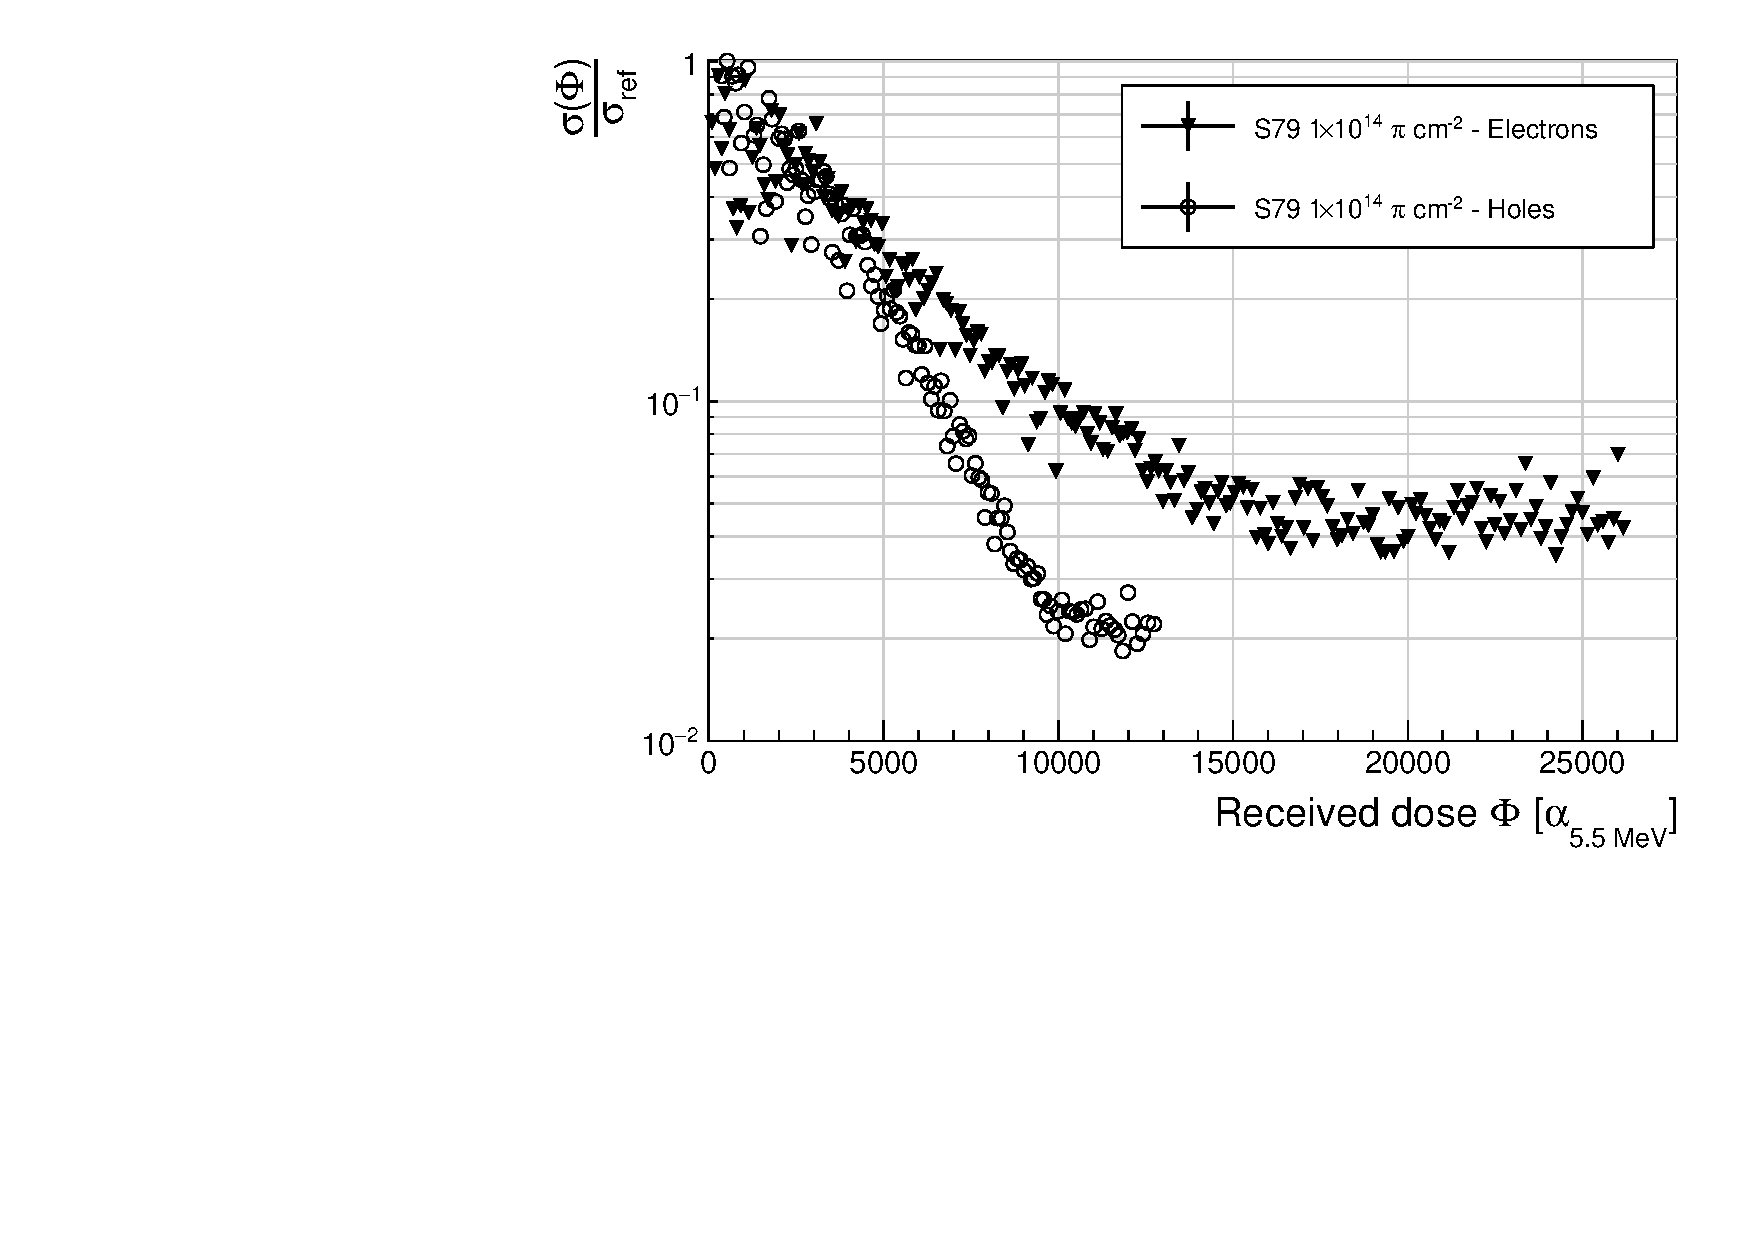
\includegraphics[width=0.8\textwidth]{03_measurement_results/scripts/plots/plotLifetime/corrlifetime}
\caption{Deterioration of the pulse shapes with time }
\label{fig:longtermc2corr}
\end{center}
\end{figure}



Finally, an effort has been made to find a way for the pulse shapes to return to their initial state. Five methods are listed: 
\begin{enumerate}[itemsep=0.1\baselineskip]
\item Removing the source and leaving the bias voltage switched on, 
\item Removing the source and switching the bias voltage off, 
\item Priming with $\upgamma$ at a rate of 400~s$^{-1}$cm$^{-1}$ without applied bias voltage, 
\item Priming with $\upbeta$ at a rate of 1000~s$^{-1}$cm$^{-1}$ with applied bias voltage and 
\item Priming with $\upbeta$ at a rate of 1000~s$^{-1}$cm$^{-1}$ without applied bias voltage. 
\end{enumerate}
The diamond sample S79 is first primed using a $^{90}$Sr source for about one hour. Then the bias voltage is switched on and an $^{241}$Am source is put on top. The pulses produced by the incident $\upalpha$ particles have a proper rectangular pulse at the beginning, but then start changing -- first gradually and later increasingly more in an erratic way, as described in the text above. After approximately 30~minutes, one of the methods is tested. When a ``healing'' procedure is started, a set of 60~pulses is taken at irregular points of time to observe the change in the pulse shape and to assess the quality of the ``healing'' procedure. Then the bias voltage is switched off and the sample is primed again to reset its state before starting with the next run. 

The results depicted in figure~\ref{fig:formCorr} show that the methods (3) and (5) improve the shape, method (2) helps slowly, (1) does not show any change with time and (4) at first improves, but then significantly degrades the shape. The effect observed in method (4) has already been described in~\cite{Kramberger:2013wva}. The ``healing'' process therefore depends on the rate of radiation, the bias voltage and the time of exposure. The ionising radiation creates free charges, which quickly recombine close to the place of generation. It is likely that they also release the charges trapped during the measurement, reducing the overall effect of the space charge. The traps get filled with both flavours of carriers, thus they are neutralised. The pulse shape gradually returns to its initial state.


\begin{footnotesize}
\begin{center}
\begin{tabular}{   c  c  c  c c }
\hline
Procedure & Source & Bias voltage & Effectiveness \\
\hline
1 & / & ON & no \\
2 & / & / & slow \\
3 & $^{60}$Co & / & YES \\
4 & $^{90}$Sr & ON & no \\
5 & $^{90}$Sr & / & YES \\
\hline
\end{tabular}
\captionof{table}{Effectiveness of healing procedures}
\label{tab:healing}
\end{center}
\end{footnotesize}

\begin{figure}[!t]
\begin{center}
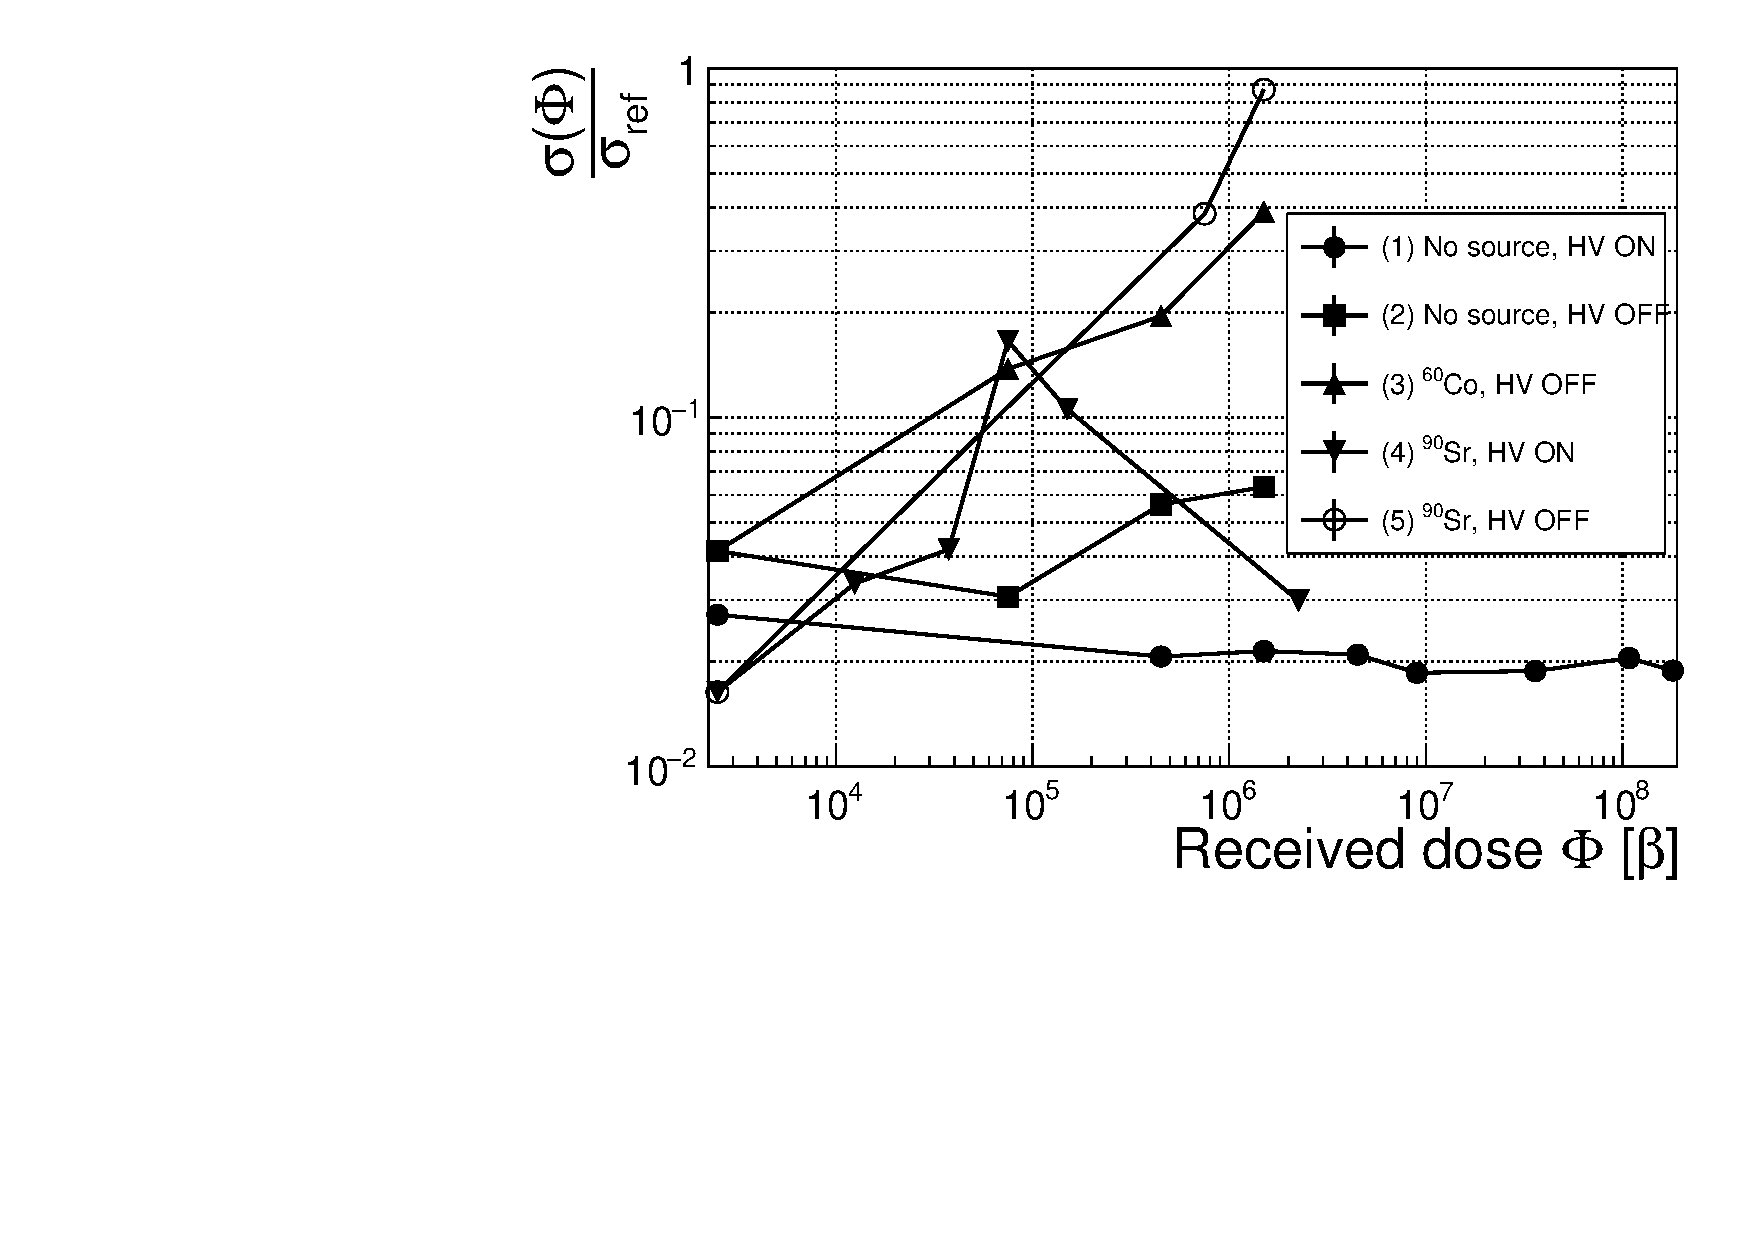
\includegraphics[width=0.8\textwidth]{03_measurement_results/scripts/plots/plotLifetime/formCorrelation}
\caption{Comparison of the five procedures for the ``healing'' process for an irradiated diamond that had been exposed to $\upalpha$ radiation with a rate of $10^1$~s$^{-1}$, with the bias voltage switched on, for at least 30~minutes.}
\label{fig:formCorr}
\end{center}
\end{figure}

%TO-DO conclusions: limitations

In summary, the shape of the pulses caused by $\upalpha$ radiation changes with time for irradiated samples. The shape of the pulses gets distorted and becomes erratic. Charge collection decreases and its spread increases. This happens even faster for non-primed diamonds. To ``heal'' the diamond -- to bring the pulse shapes back to their initial shape -- the sample must be primed using a $\upbeta$ or a $\upgamma$ source for several minutes at the bias voltage set to 0~V. Switching to the inverse polarity for a few seconds helps a bit, but in a long run distorts the signal, which cannot get back to its initial shape.

















% ---------------------------------------------------------------------------------------------------------------
%\clearpage
\section{Temperature limitations}
\label{sec:templimit}
% ---------------------------------------------------------------------------------------------------------------
A test has been carried out to evaluate the effect of temperature changes on the output signal of the diamond sensors. A cryostat filled with liquid helium is used to cool down the sensor during the measurement process. The current signal response to $\alpha$-particles is measured at 18 temperature points between 4~K and 295~K. At every temperature point, a set of 300 pulses is read out at various bias voltages. Resulting data show that the charge collection is stable down to 150~K, where it starts decreasing and stabilises again at about one third of the initial value at 75~K. This behaviour was first measured and discussed by H. Jansen~\cite{Jansen:1956431}.

%\subsubsection{Acoustic phonon scattering}
The band gap energy in diamond is equal to $E_\mathrm{g}=5.5$~eV while the average energy to produce an electron-hole pair is $E_{\mathrm{e-h}}=13.25$~eV. This means there is excessive energy deposited in the diamond bulk. The incident $\upalpha$-particle stops within $\sim$10--15~$\upmu$m of the bulk, transferring all its energy to the lattice during deceleration. A part of this energy directly ionises the carbon atoms, creating free electron-hole pairs. The positively charged hole and the negatively charged electron in the hole attract each other via the Coulomb force and may undergo a bonding process during which a phonon is emitted. 

The remaining energy, however, is converted into lattice vibrations (phonons~\cite{PhysRevLett.13.13, Jansen:1956431}). This means that the lattice within the ionisation volume (approximately $\sim$15~$\upmu$m$\times\sim$2~nm in size) is briefly heated up. The hot plasma then cools down to the temperature of the surrounding material by heat dissipation, (i.e. phonon transport).
%\subsubsection{Exciton formation and recombination}
%That phonon is referred to as \emph{exciton}~\cite{Exciton}. 
The free electron binds the free hole into a bound state (not recombination) -- the exciton~\cite{1970PhyEd...5..226L}. The exciton binding energy is 80~meV. At higher temperatures, the lattice provides enough energy to excite the electron from the exciton state back to the conduction band. At lower temperatures, however, the exciton lifetime increases, which means that it will take a longer time for the electrons to get re-excited to the conduction band. The re-excitation lifetime at room temperature is $\sim$30~ps, increasing to $\sim$150~$\upmu$s at 50~K~\cite{Jansen:1956431}. This means that some of the bound electrons will not even start drifting within the period of $\sim$10~ns, which is the expected carrier drift time. When they are finally freed, the current they induce is already hidden in the electronics noise. The effective area of the observed current pulse is therefore smaller than that of a pulse induced by all the carriers drifting at the same time. This in effect reduces the measured collected charge. The longer the time constant, the lower the measured collected charge, as shown in figure~\ref{fig:chgtemp} below.


%The irradiated samples were put in the cryostat, which was cooled down to 4.2~K using liquid helium. TCT data were then taken at a range of bias voltages at temperature points ranging between 4.2~K and room temperature (RT). The results showed that irradiation causes forming of charge traps in the bulk.l;'
%
%TO-DO: get the Tau and plot it against T. 
%TO-DO: plot the drift time against square voltage.


\subsection{Temperature-variant $\upalpha$-TCT before irradiation}
% Show a set of pulses
Three sCVD diamond samples have been tested at a range of temperatures using the $\upalpha$-TCT technique. At each temperature point, the bias voltage is set to several positive and negative values. A set of 300 pulses is recorded at every data point and averaged offline. The resulting averaged pulses of sample S37 at the 260~K temperature point and a bias voltage of $\pm$400~V, $\pm$500~V and $\pm$700~V are shown in figure~\ref{fig:voltpulse}. The pulses induced by holes as charge carriers are shorter than those induced by electrons, which means that holes travel faster in diamond. The area of the pulse, however, is the same for both polarities, which corresponds to the fact that the same amount of charges is drifting in both cases.

\begin{figure}[!t]
\begin{tabular}{rr}
\subfloat{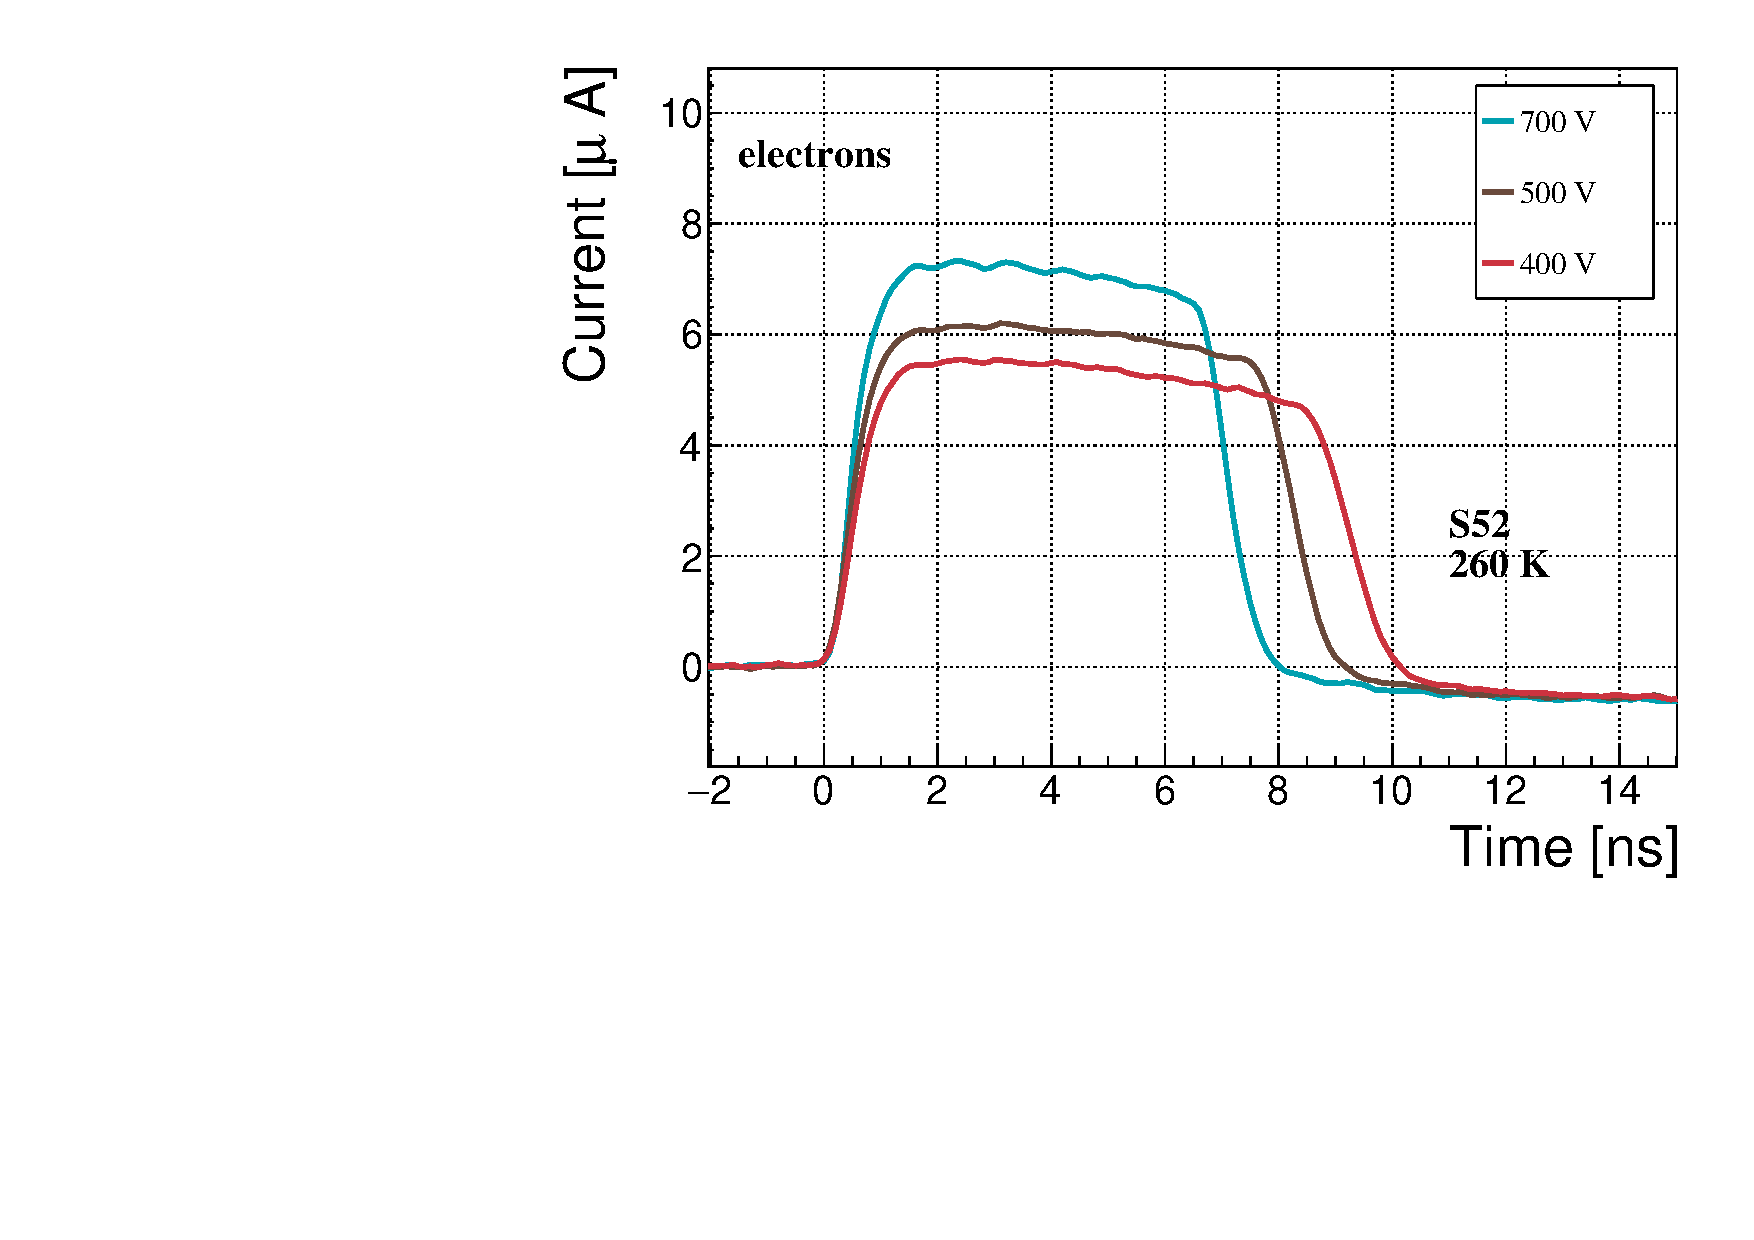
\includegraphics[width=0.47\textwidth]{03_measurement_results/scripts/plots/pulsesVolt/varVolt_S52_elecs_260k} \label{fig:S52cTplus}} &
\subfloat{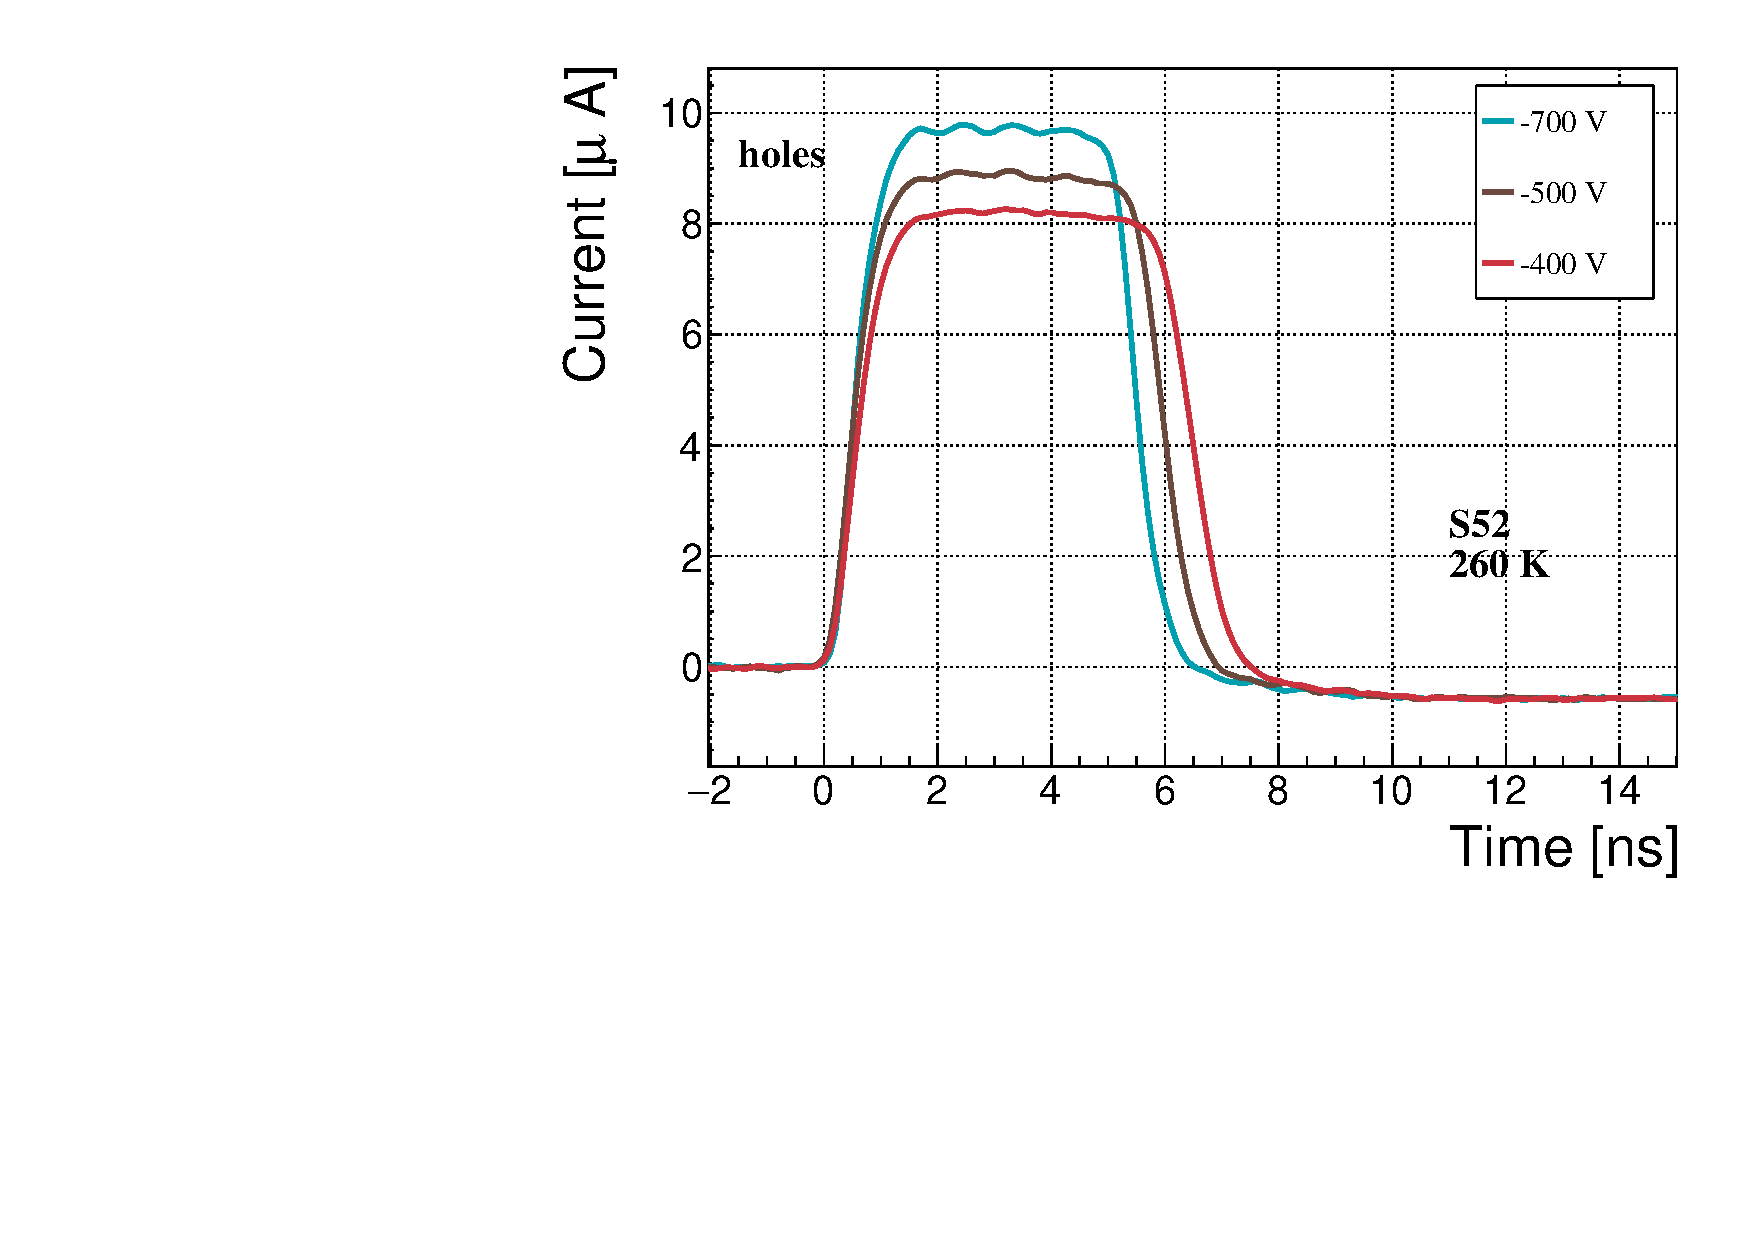
\includegraphics[width=0.47\textwidth]{03_measurement_results/scripts/plots/pulsesVolt/varVolt_S52_holes_260k}  \label{fig:S52ctTminus}}
\end{tabular}
\caption{Varied bias voltage at a fixed temperature}
\label{fig:voltpulse}
\end{figure}

Figure~\ref{fig:temppulses} shows pulses at a bias voltage set to $\pm500$~V across the range of temperatures between 4~K and 295~K -- room temperature (RT). Several conclusions can be drawn by observing their shape. First, the pulse shapes change with decreasing temperature. The pulse time gets shorter, hinting at the faster carrier drift velocity $v_{\mathrm{drift}}$. Second, between 150~K and 75~K there is a significant change in shape - the time constant of the rising edge increases significantly and the pulse area decreases. From 75~K down to 4~K there is no significant observable change. Last, the top of the pulse at the S52 is not flat, which means that a portion of the drifting charge is lost along its way.  This is due to charge trapping, likely by means of crystal defects or impurities.	

%This could be due to impurities in the diamond bulk, which act as charge traps, or due to the space charge built up in the bulk. A linear pulse top hints on the latter. All in all, the pulse shape changes significantly with temperature, which is predicted by Jansen's model.

\begin{figure}%[!t]
\begin{tabular}{rr}
\subfloat{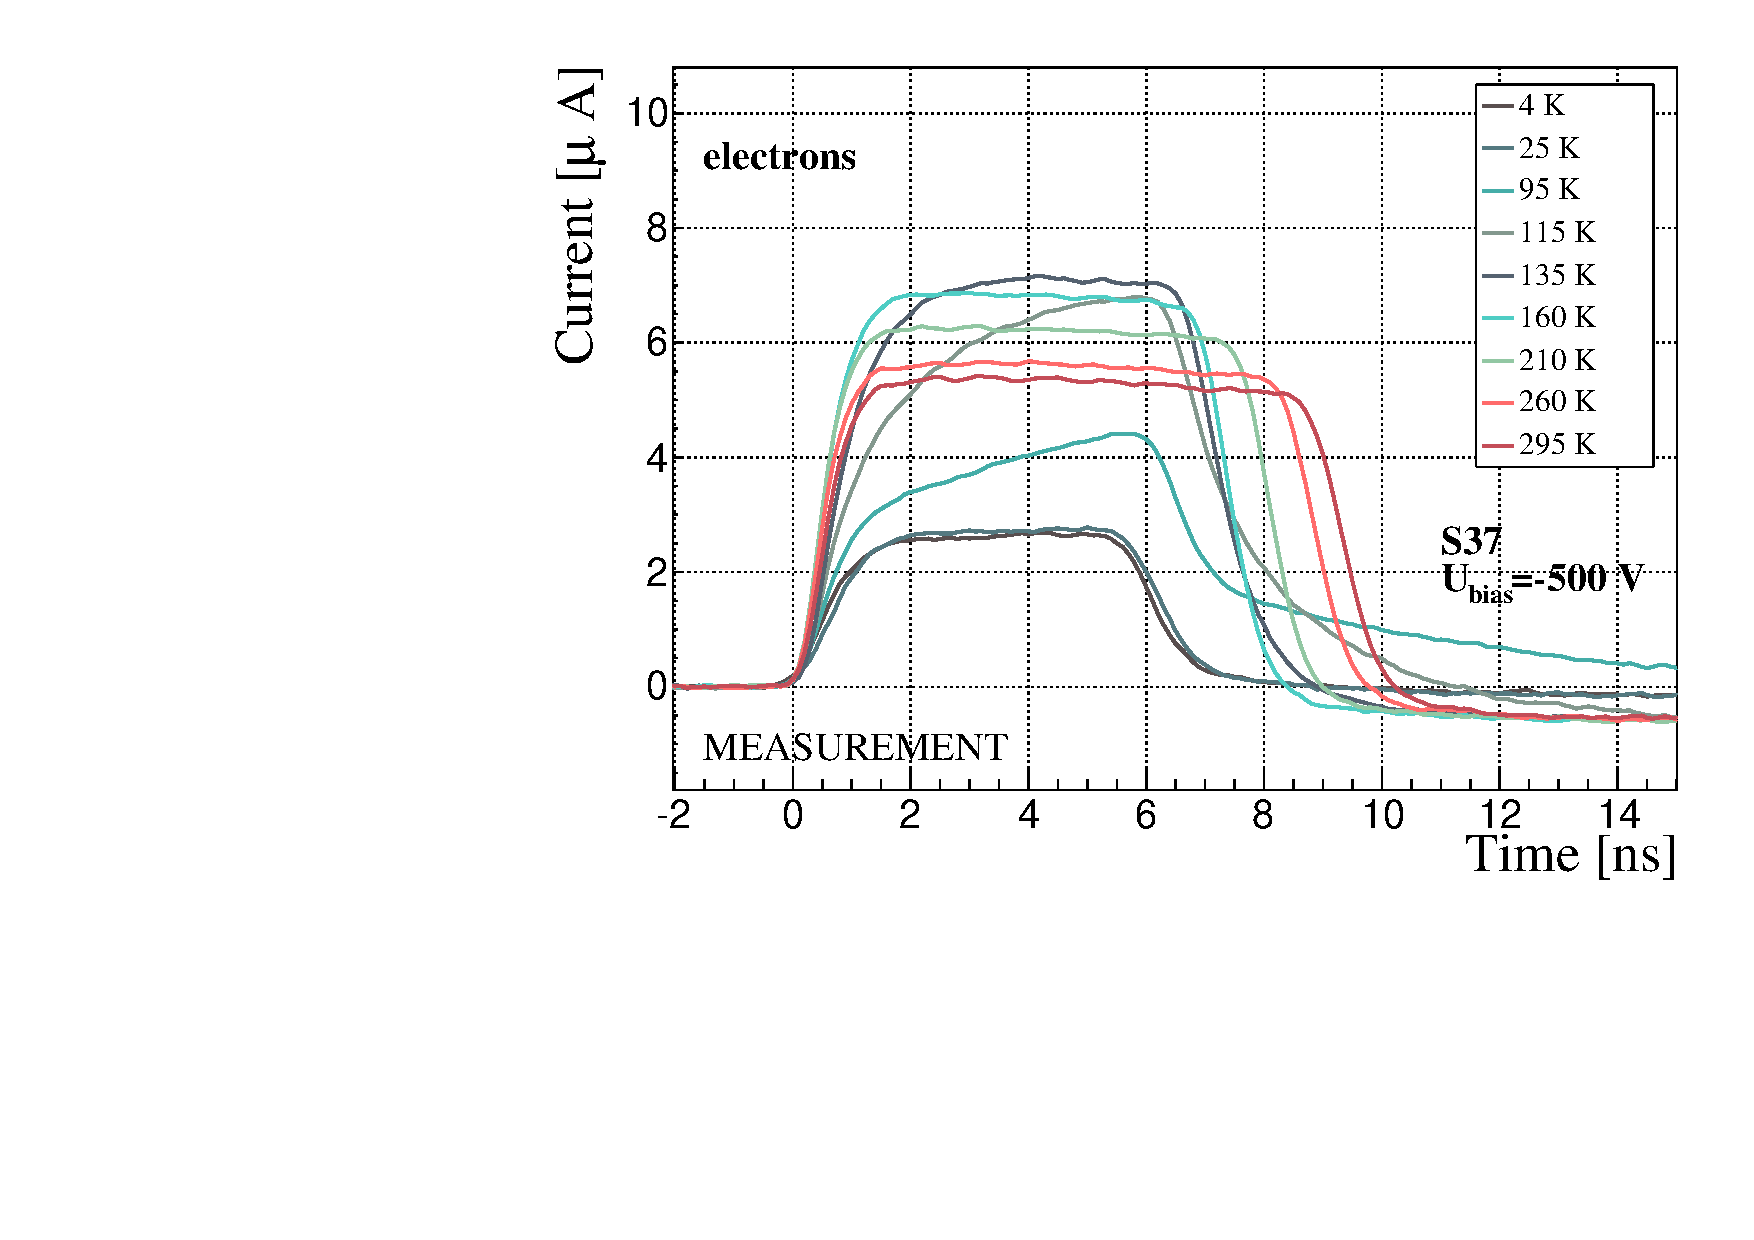
\includegraphics[width=0.47\textwidth]{03_measurement_results/scripts/plots/pulses/S37_elecs} \label{fig:S37plus}} &
\subfloat{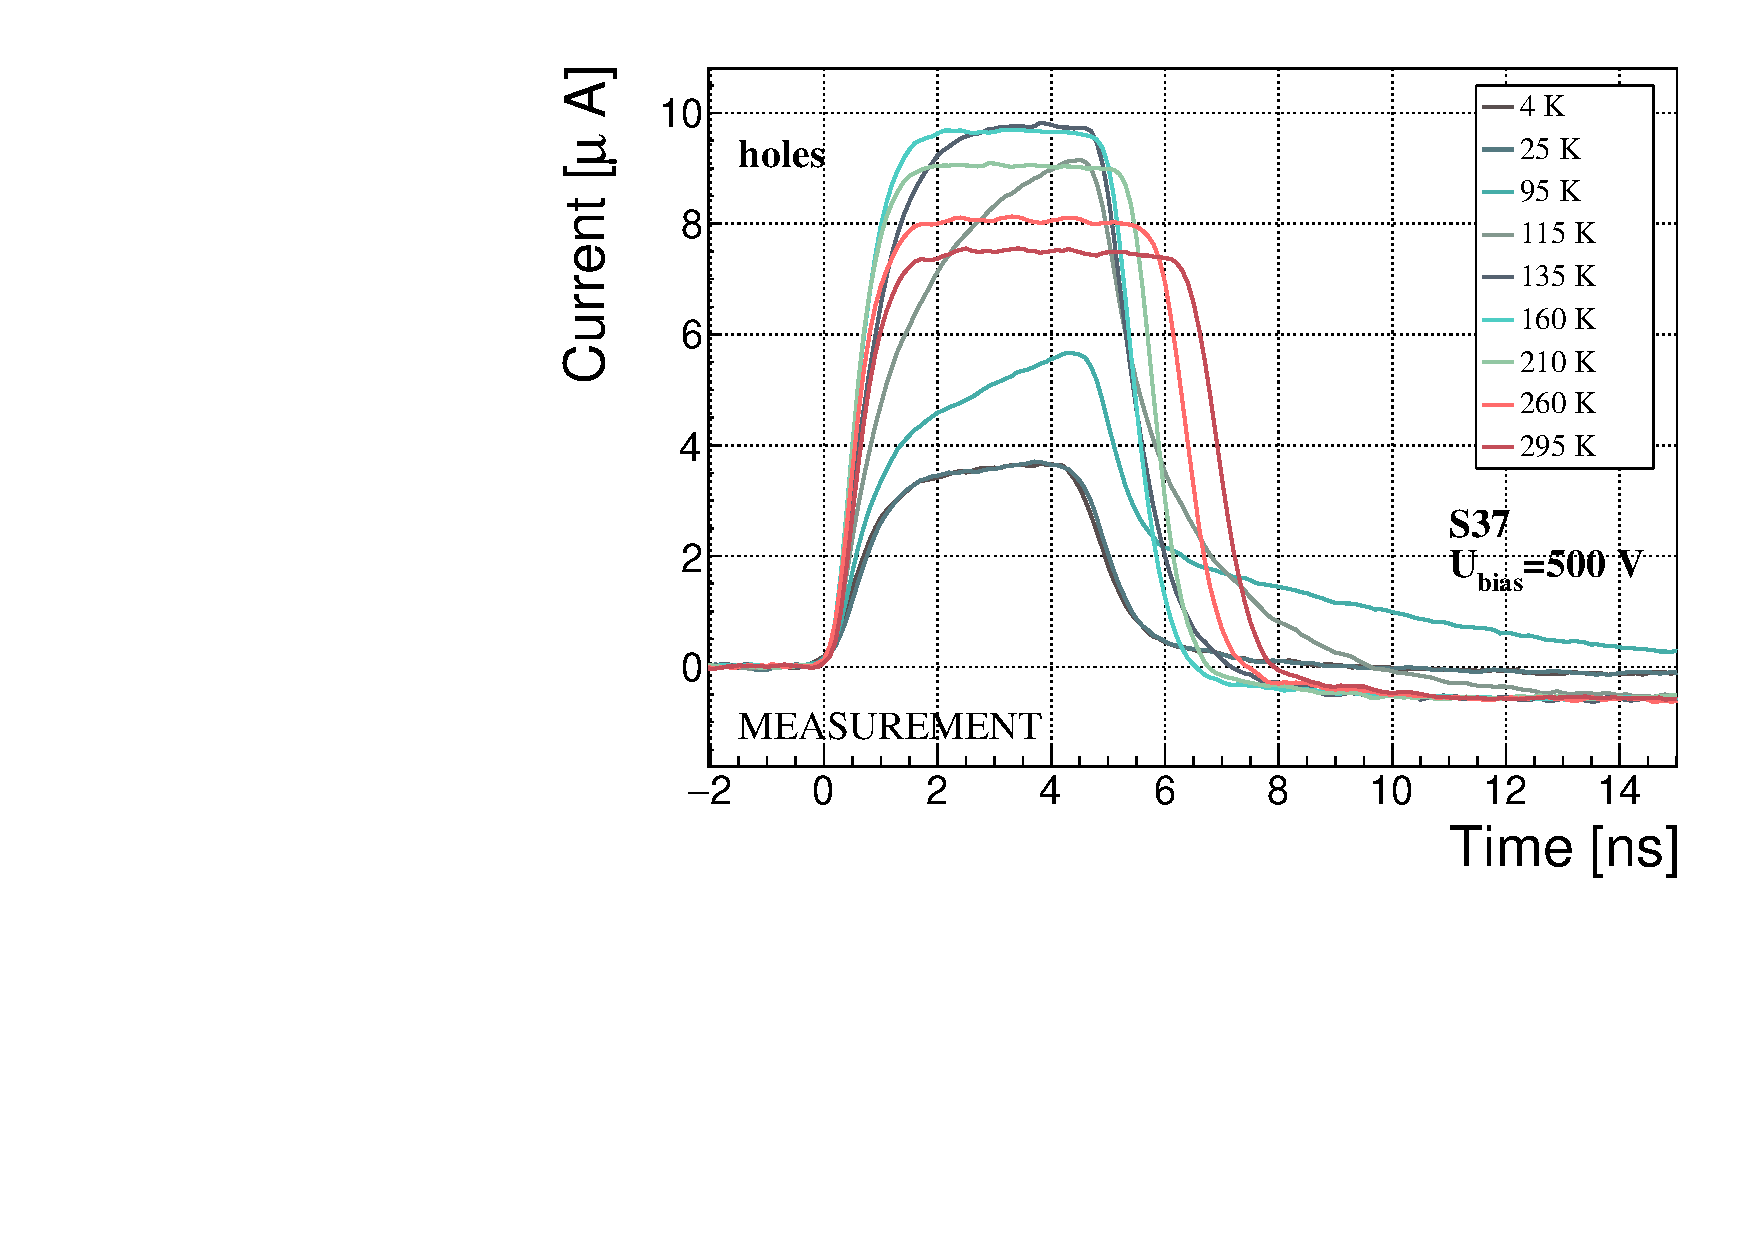
\includegraphics[width=0.47\textwidth]{03_measurement_results/scripts/plots/pulses/S37_holes}  \label{fig:S37minus}} \\
\subfloat{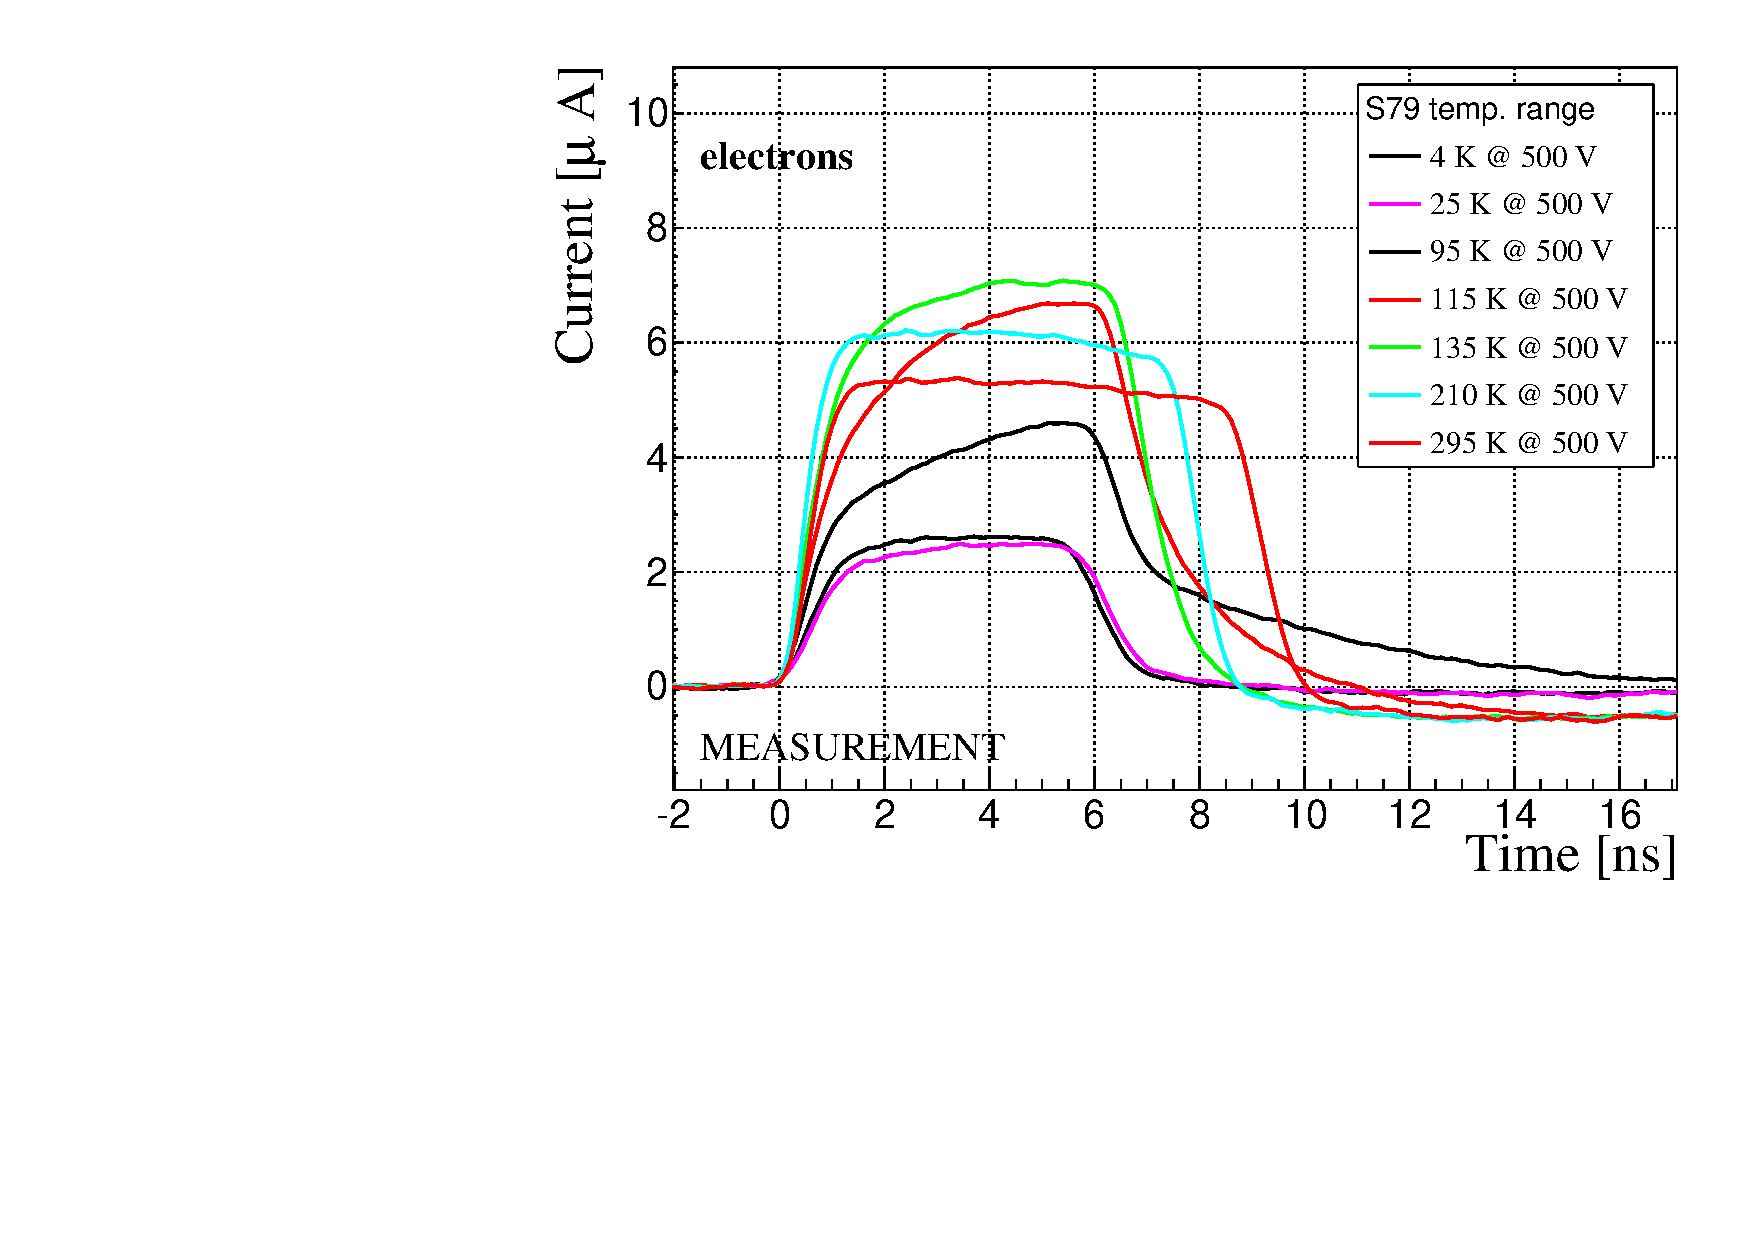
\includegraphics[width=0.47\textwidth]{03_measurement_results/scripts/plots/pulses/S79_elecs} \label{fig:S79plus}} &
\subfloat{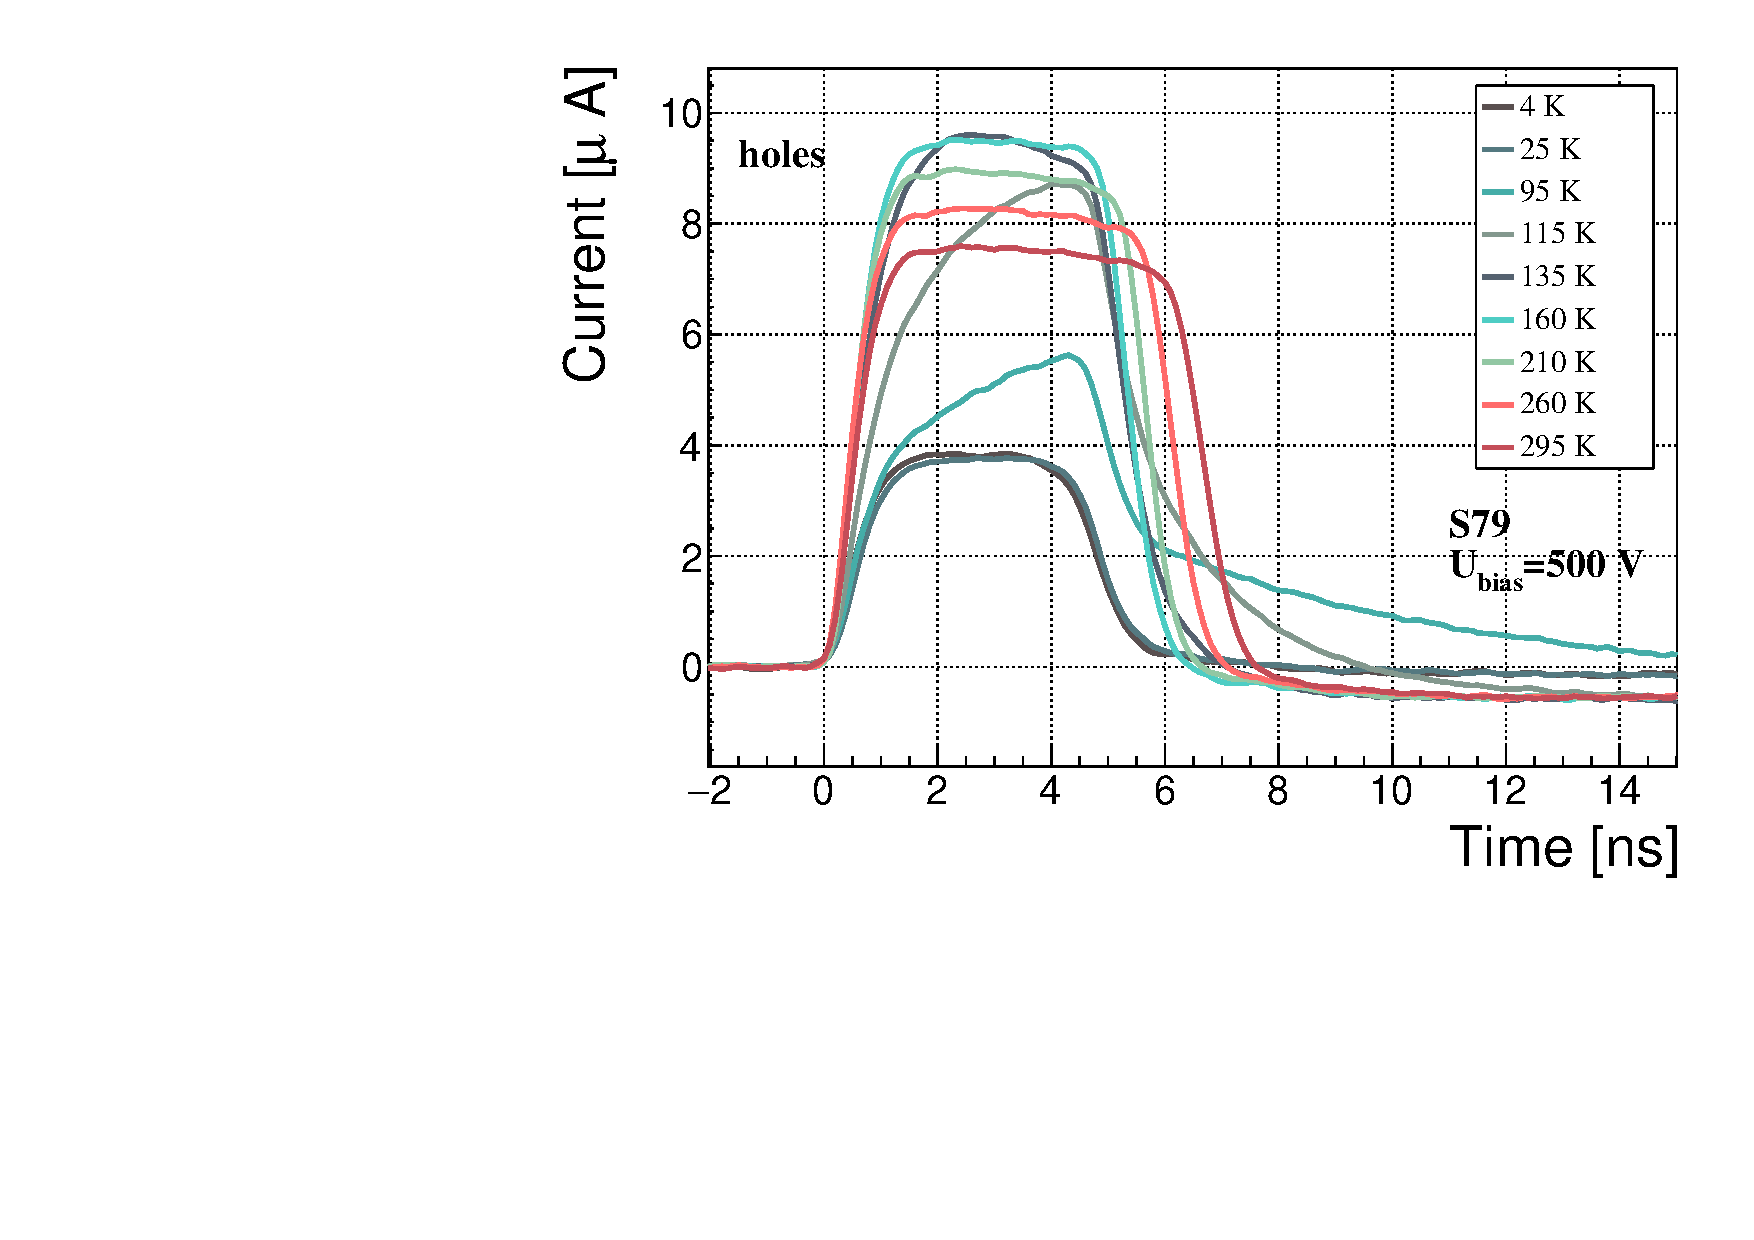
\includegraphics[width=0.47\textwidth]{03_measurement_results/scripts/plots/pulses/S79_holes}  \label{fig:S79minus}} \\
\subfloat{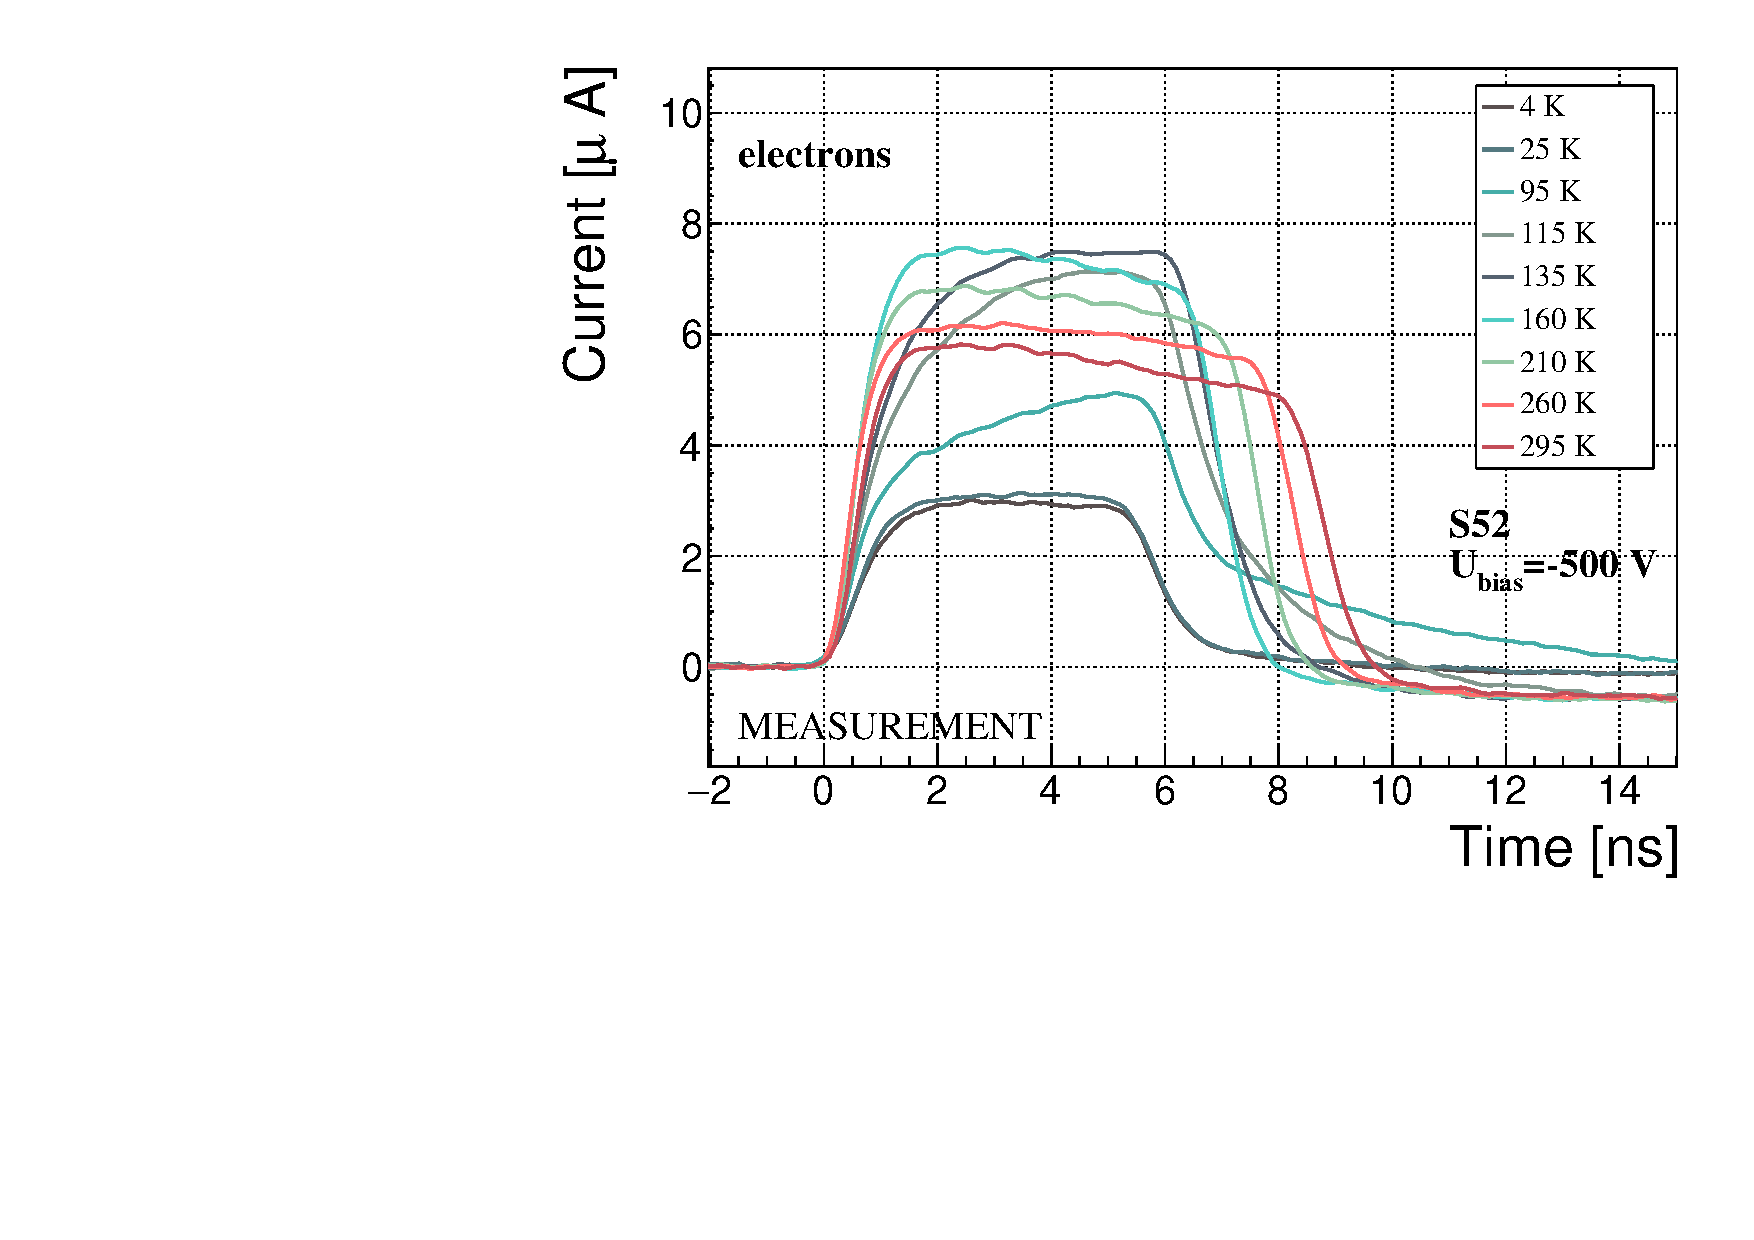
\includegraphics[width=0.47\textwidth]{03_measurement_results/scripts/plots/pulses/S52_elecs} \label{fig:S52plus}} &
\subfloat{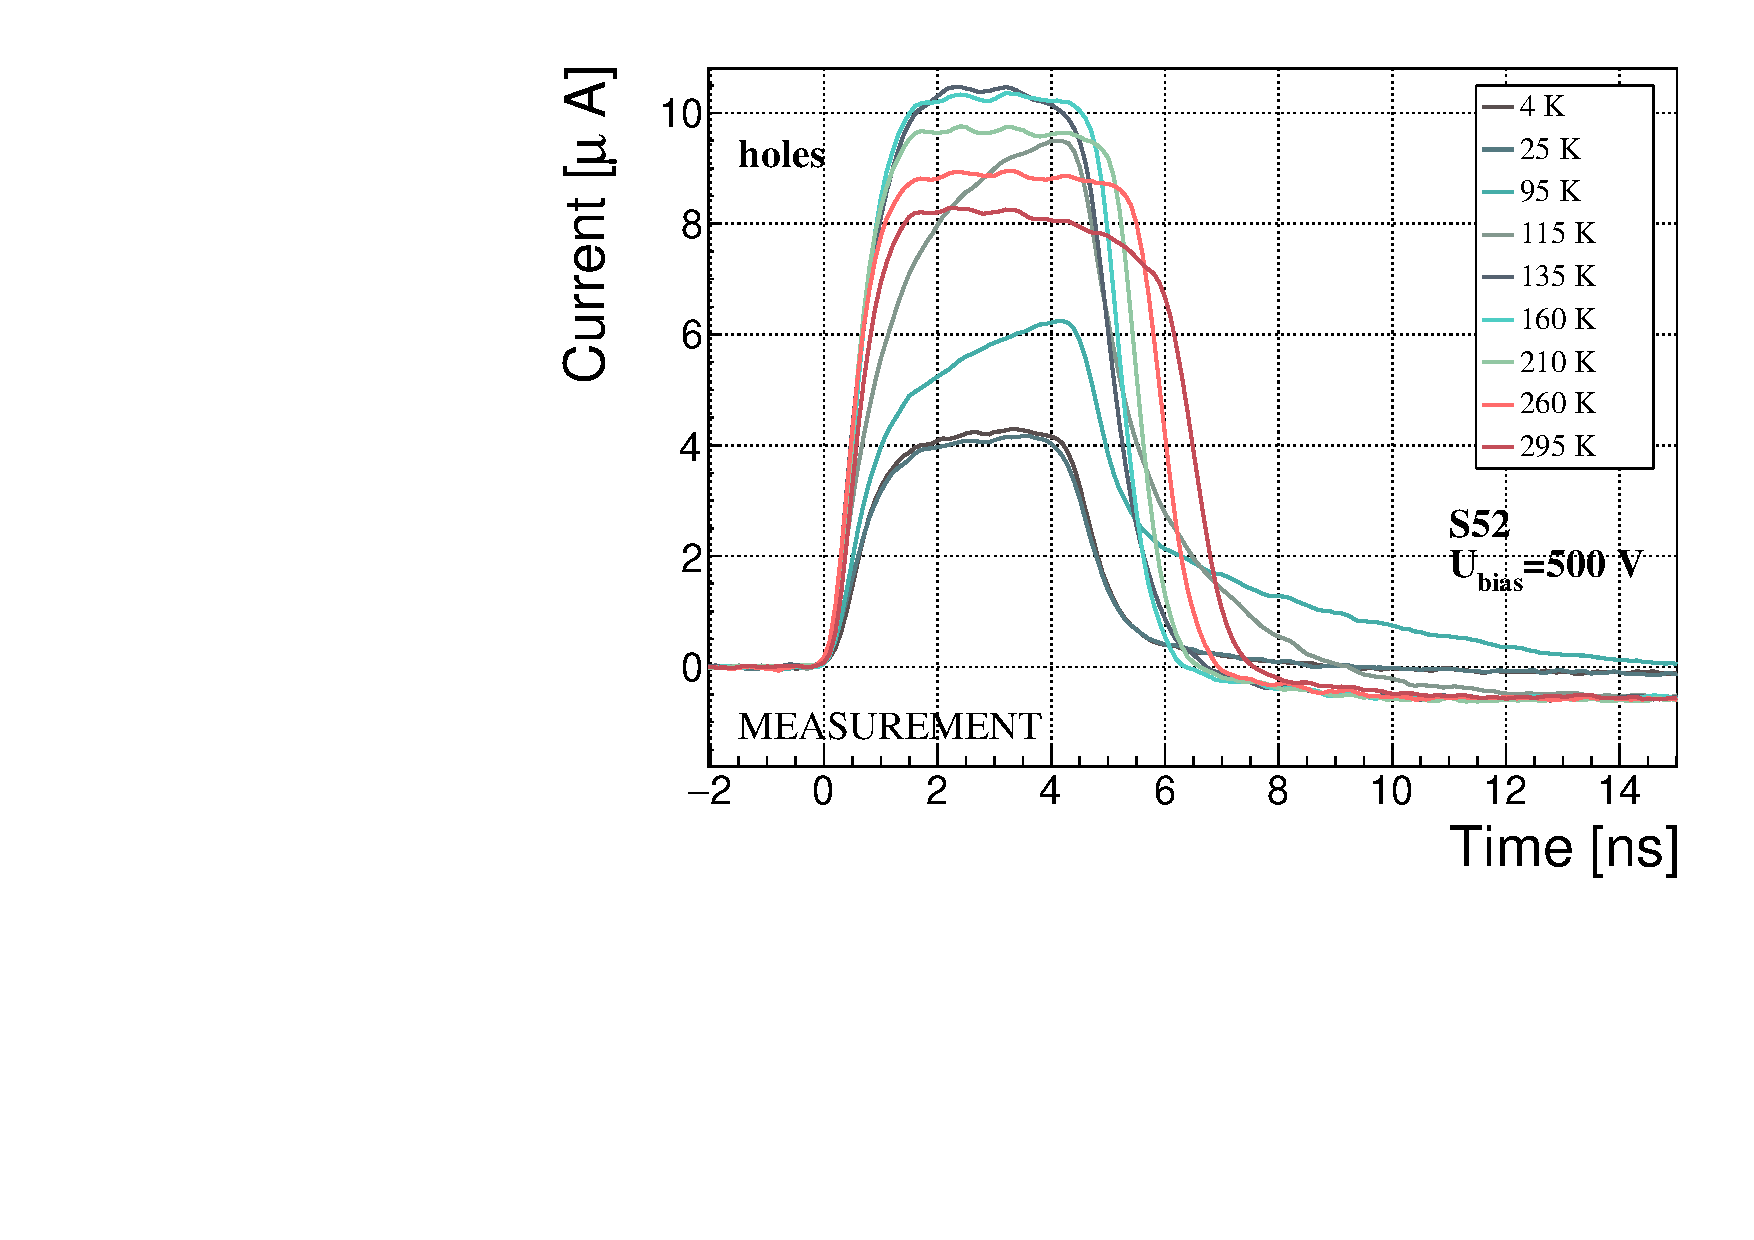
\includegraphics[width=0.47\textwidth]{03_measurement_results/scripts/plots/pulses/S52_holes}  \label{fig:S52minus}}
\end{tabular}
\caption{Several data points between 4~K and 295~K at a bias voltage of $\pm$500~V}
\label{fig:temppulses}
\end{figure}


% TO-DO Show drift velocity wrt volt
% TO-DO Show drift velocity wrt temp
% TO-DO Show integrated charge
% TO-DO Show Vdrift wrt 1/Voltage
%$(1\pm0.2)\times10^{14}~\pi~cm^{-2}$ and $(3.63\pm0.76)\times10^{14}~\pi~cm^{-2}$. 

\subsection{Temperature-variant $\upalpha$-TCT after irradiation}
The irradiated S79 and S52 have been re-tested in the cryostat after irradiation. The aim was to see how their pulse shapes change with decreasing temperature, in particular the decaying top of the pulses (see figure~\ref{fig:voltpulseAfter}). The decay time gives information on trapping of charge carriers while travelling through the diamond bulk. A variation of the decay time constant as a function of temperature might help to reveal the type and depth of the charge traps. To observe these effects or lack thereof, a number of requirements has to be met. First, the diamond samples are intentionally not primed prior to the experiment because priming would improve the pulse shapes and possibly change the decay time constant of the signal. Second, keeping in mind that the pulse shape of irradiated diamonds changes with time, the duration of the measurement of an individual data point has to be short -- of the order of 30~seconds. Last, the sequence of the bias voltage settings is important, the reason for which is explained below.

Unfortunately it is not possible to avoid temporal pulse changes. For instance, one measurement point takes approximately one minute. After the measurement, the bias voltage polarity is swapped for a few seconds to bring the diamond back into its initial state. But a few seconds with respect to a minute is not enough. Therefore, when the bias voltage is set to the next value, there is still some residual effect of the previous measurement. Similar to the effects of polarisation, this effect is also decreasing the pulse height. This can be observed in figure~\ref{fig:voltpulseAfter}, which shows the resulting pulses of S52 for bias voltages of $\pm$200~V, $\pm$300~V, $\pm$400~V and $\pm$500~V at 230~K and 260~K. In this case the measurements sequence is: 230K (200~V, 300~V, 400~V, 500~V, -500~V, -400~V, -300~V), 260~K (-200~V, -300~V, -400~V, -500~V, 500~V, 400~V, 300~V). The changes in pulse shapes for holes at 230~K and 260~K cannot be attributed to the temperature change. Instead, the explanation could lie in diamond ``polarisation''. This means that, when exposed to an electric field with $\upalpha$ measurements ongoing, the diamond builds up an internal electric field of inverse polarity, which effectively reduces the overall electric field. This internal field does not dissipate when the external bias voltage is switched off. It can be said that the diamond becomes ``polarised''. When switching the polarity of the external bias voltage, the internal and external electric field point in the same direction at the beginning, increasing the overall electric field and with it the pulse height. In figure~\ref{fig:voltpulseAfter}, this happens when switching from 500~V (figure~\ref{fig:S52cTplusAfter230}) to -500~V (figure~\ref{fig:S52cTminusAfter230}) at 230~K. The built up polarisation contributes to the pulse having a sharp rising edge and a high amplitude. This effect decays during the next two voltage points. There would be a handful of ways to avoid this polarisation effect in the data: 

\begin{enumerate}[itemsep=0.1\baselineskip]
\item After every data point invert the bias voltage and leave it to return to a neutral state for the same amount of time, 
\item Make a hysteresis of data points, going from minimum negative to maximum positive bias several times, 
\item Reduce the measurement time at every bias voltage setting.
\end{enumerate}
Unfortunately, options (1) and (2) are very time consuming and would increase the overall experiment time to over one day. The third option would worsen the resulting averaged pulses. In the end an alternative option was chosen: alternating the starting bias voltage and the sequence at every temperature point. With this option, a meaningful systematic error in analysing the pulse shapes can be attained.

\begin{figure}[!t]
\begin{tabular}{rr}
\subfloat{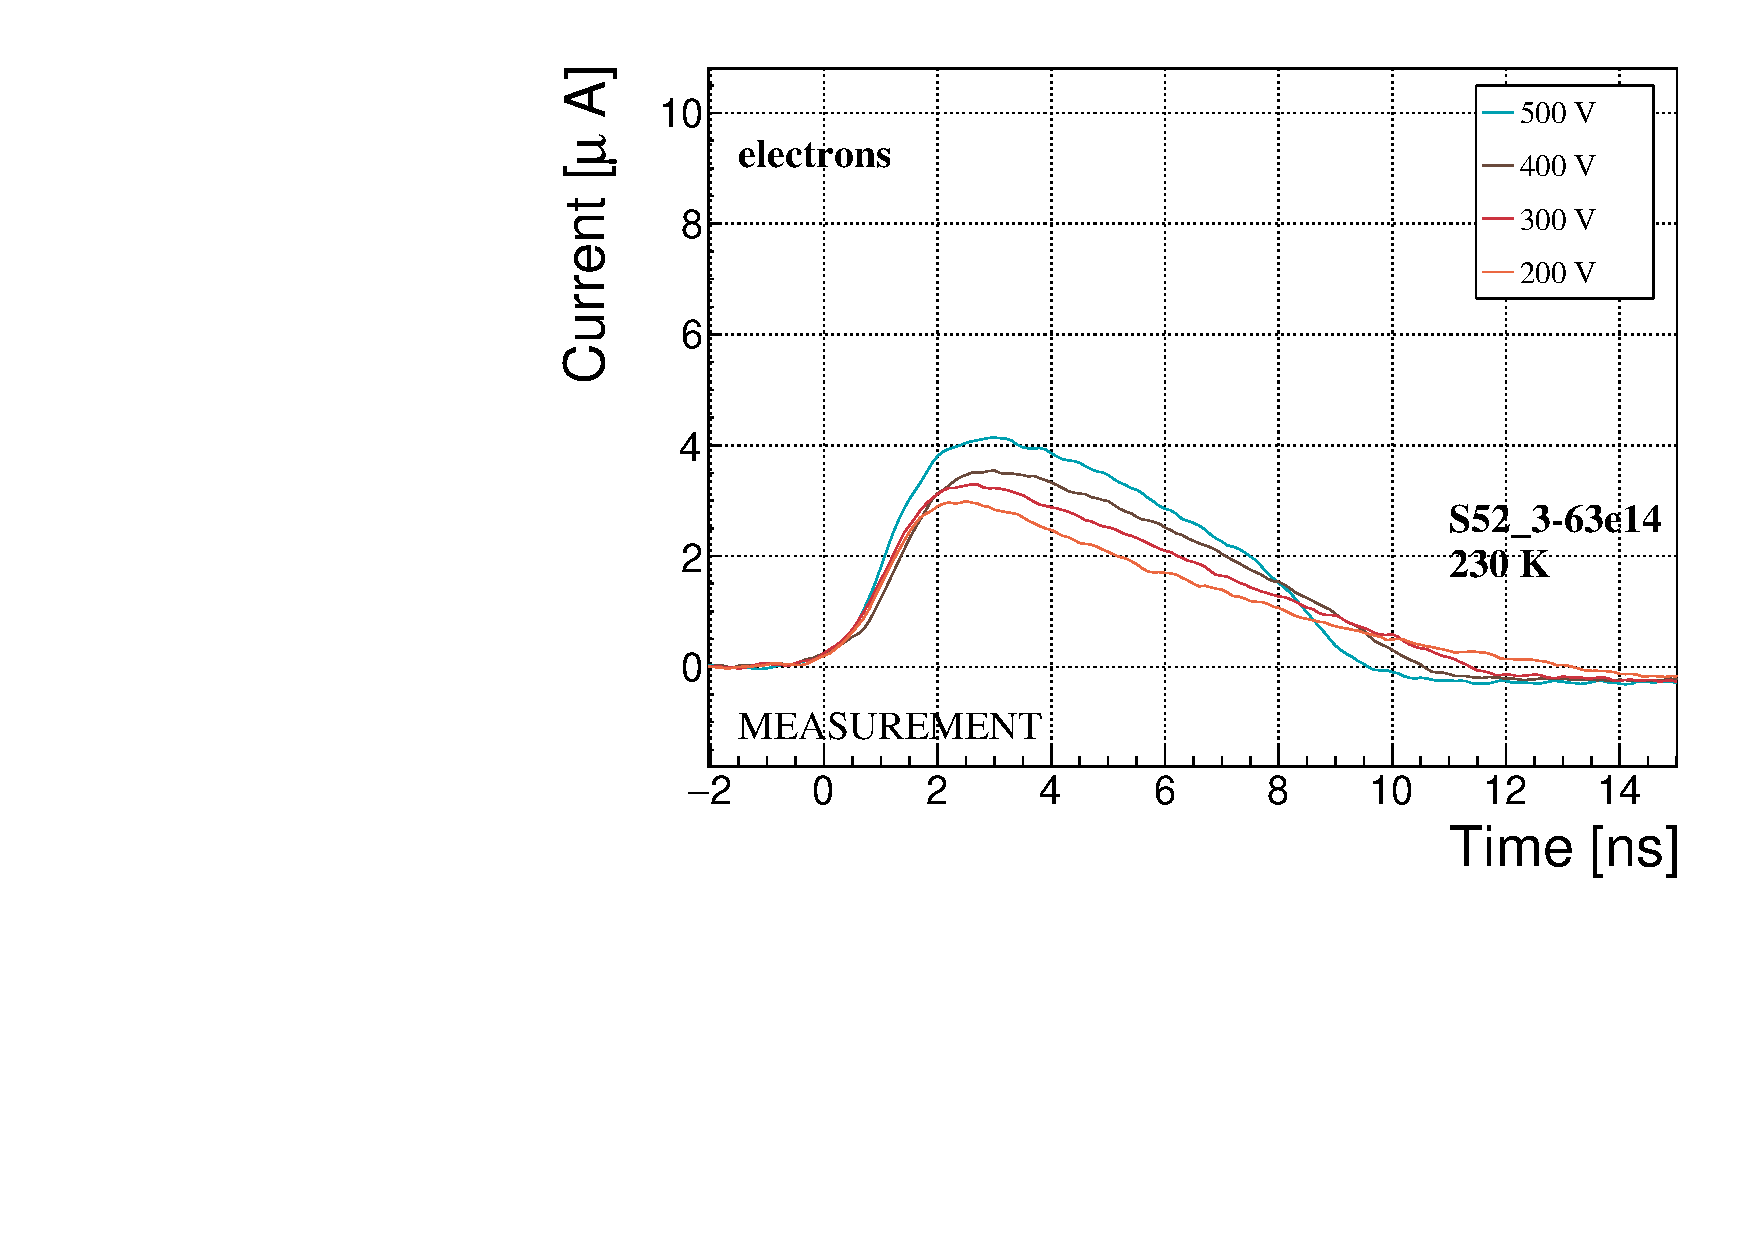
\includegraphics[width=0.47\textwidth]{03_measurement_results/scripts/plots/pulsesVolt/varVolt_S52_3-63e14_elecs_230k} \label{fig:S52cTplusAfter230}} &
\subfloat{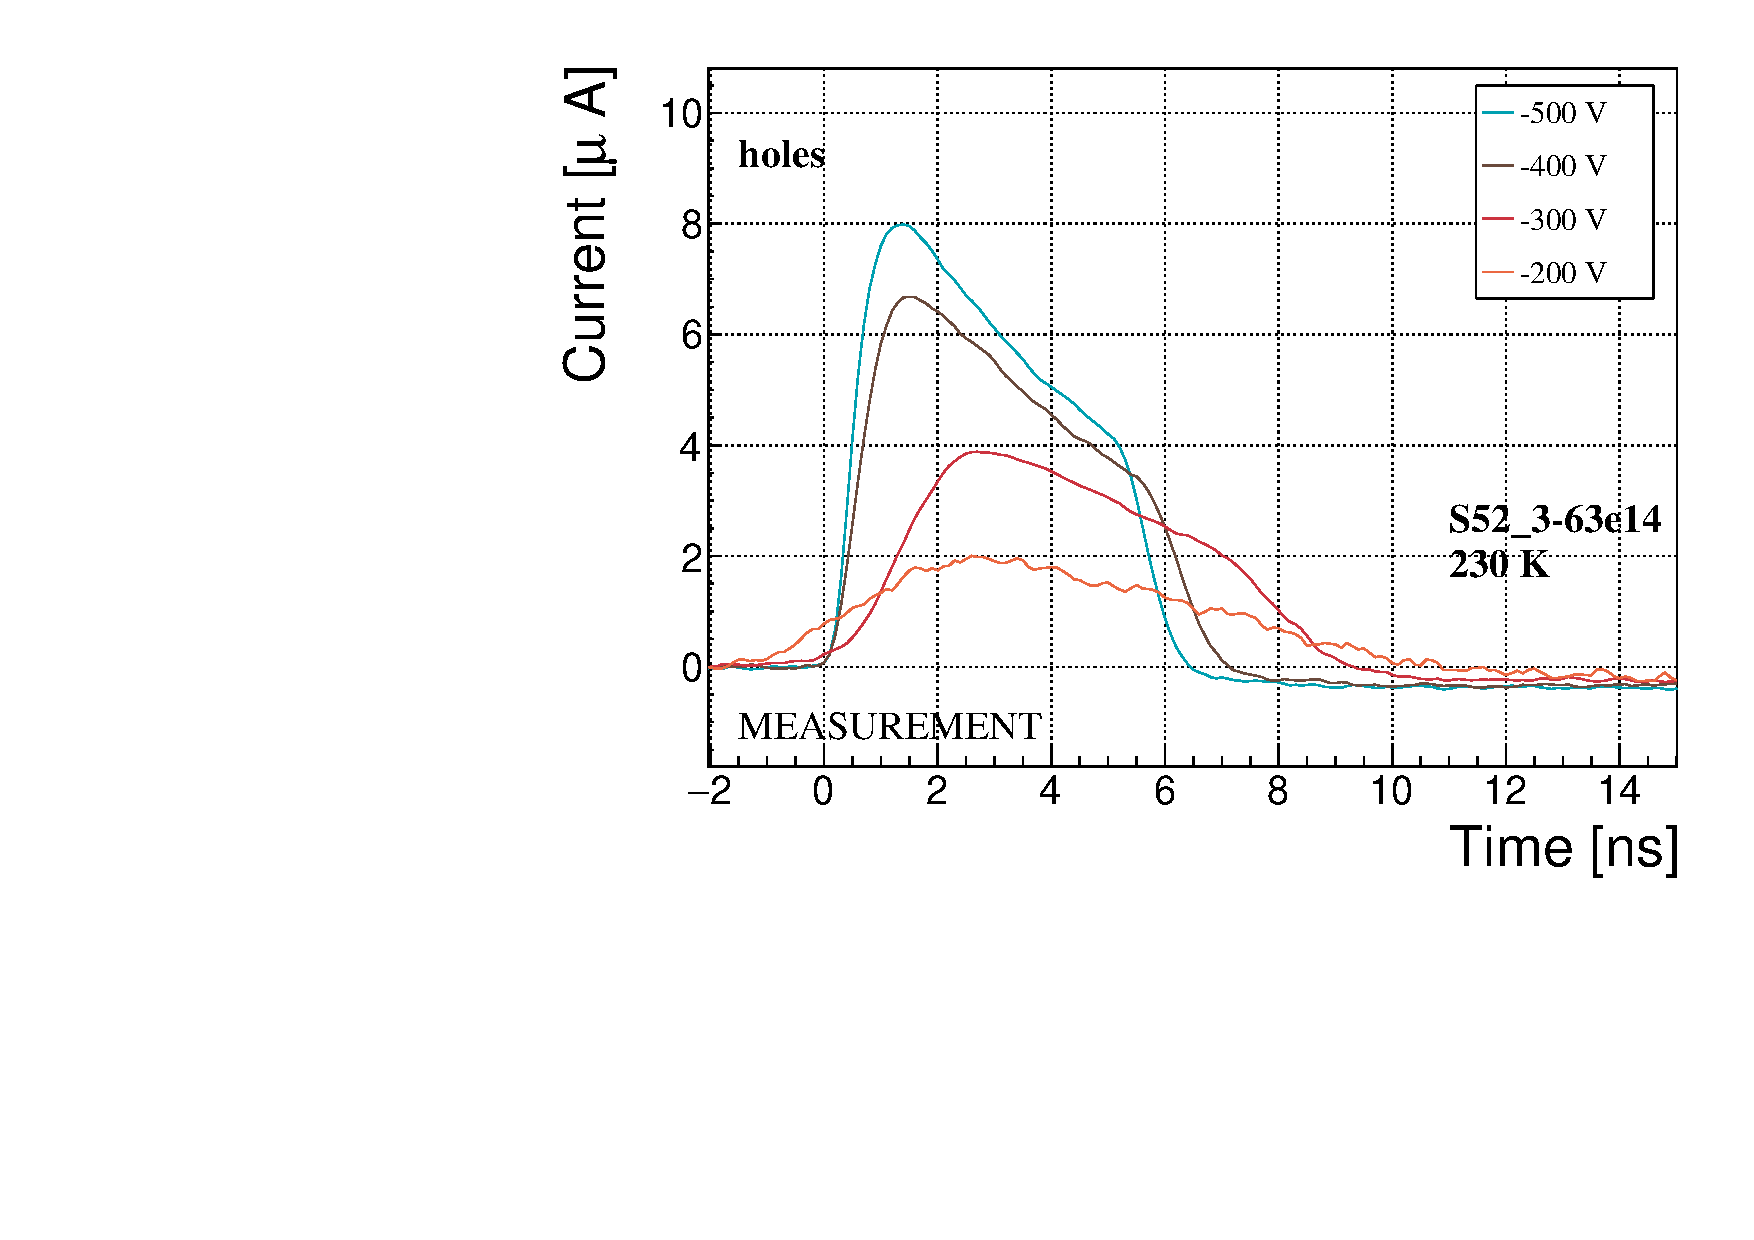
\includegraphics[width=0.47\textwidth]{03_measurement_results/scripts/plots/pulsesVolt/varVolt_S52_3-63e14_holes_230k}  \label{fig:S52ctTminusAfter230}} \\
\subfloat{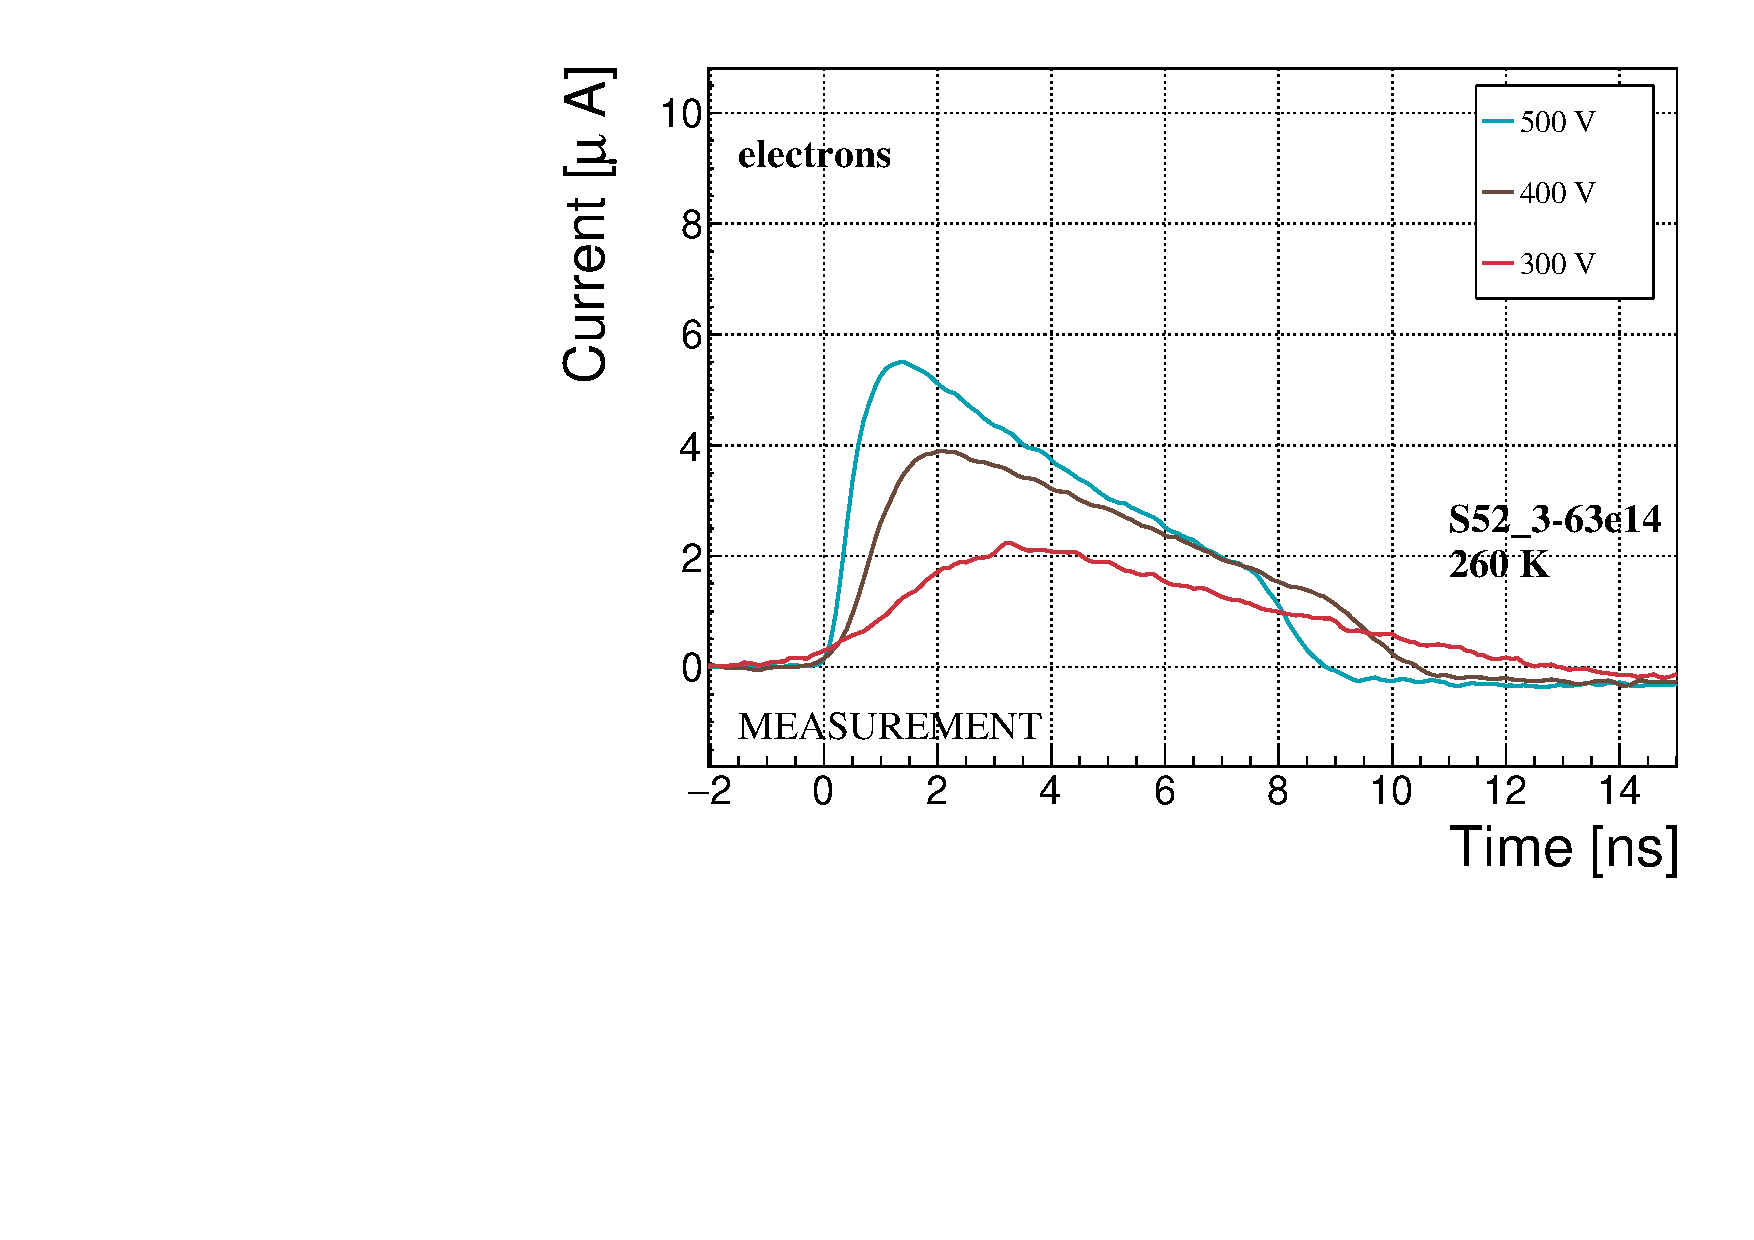
\includegraphics[width=0.47\textwidth]{03_measurement_results/scripts/plots/pulsesVolt/varVolt_S52_3-63e14_elecs_260k} \label{fig:S52cTplusAfter260}} &
\subfloat{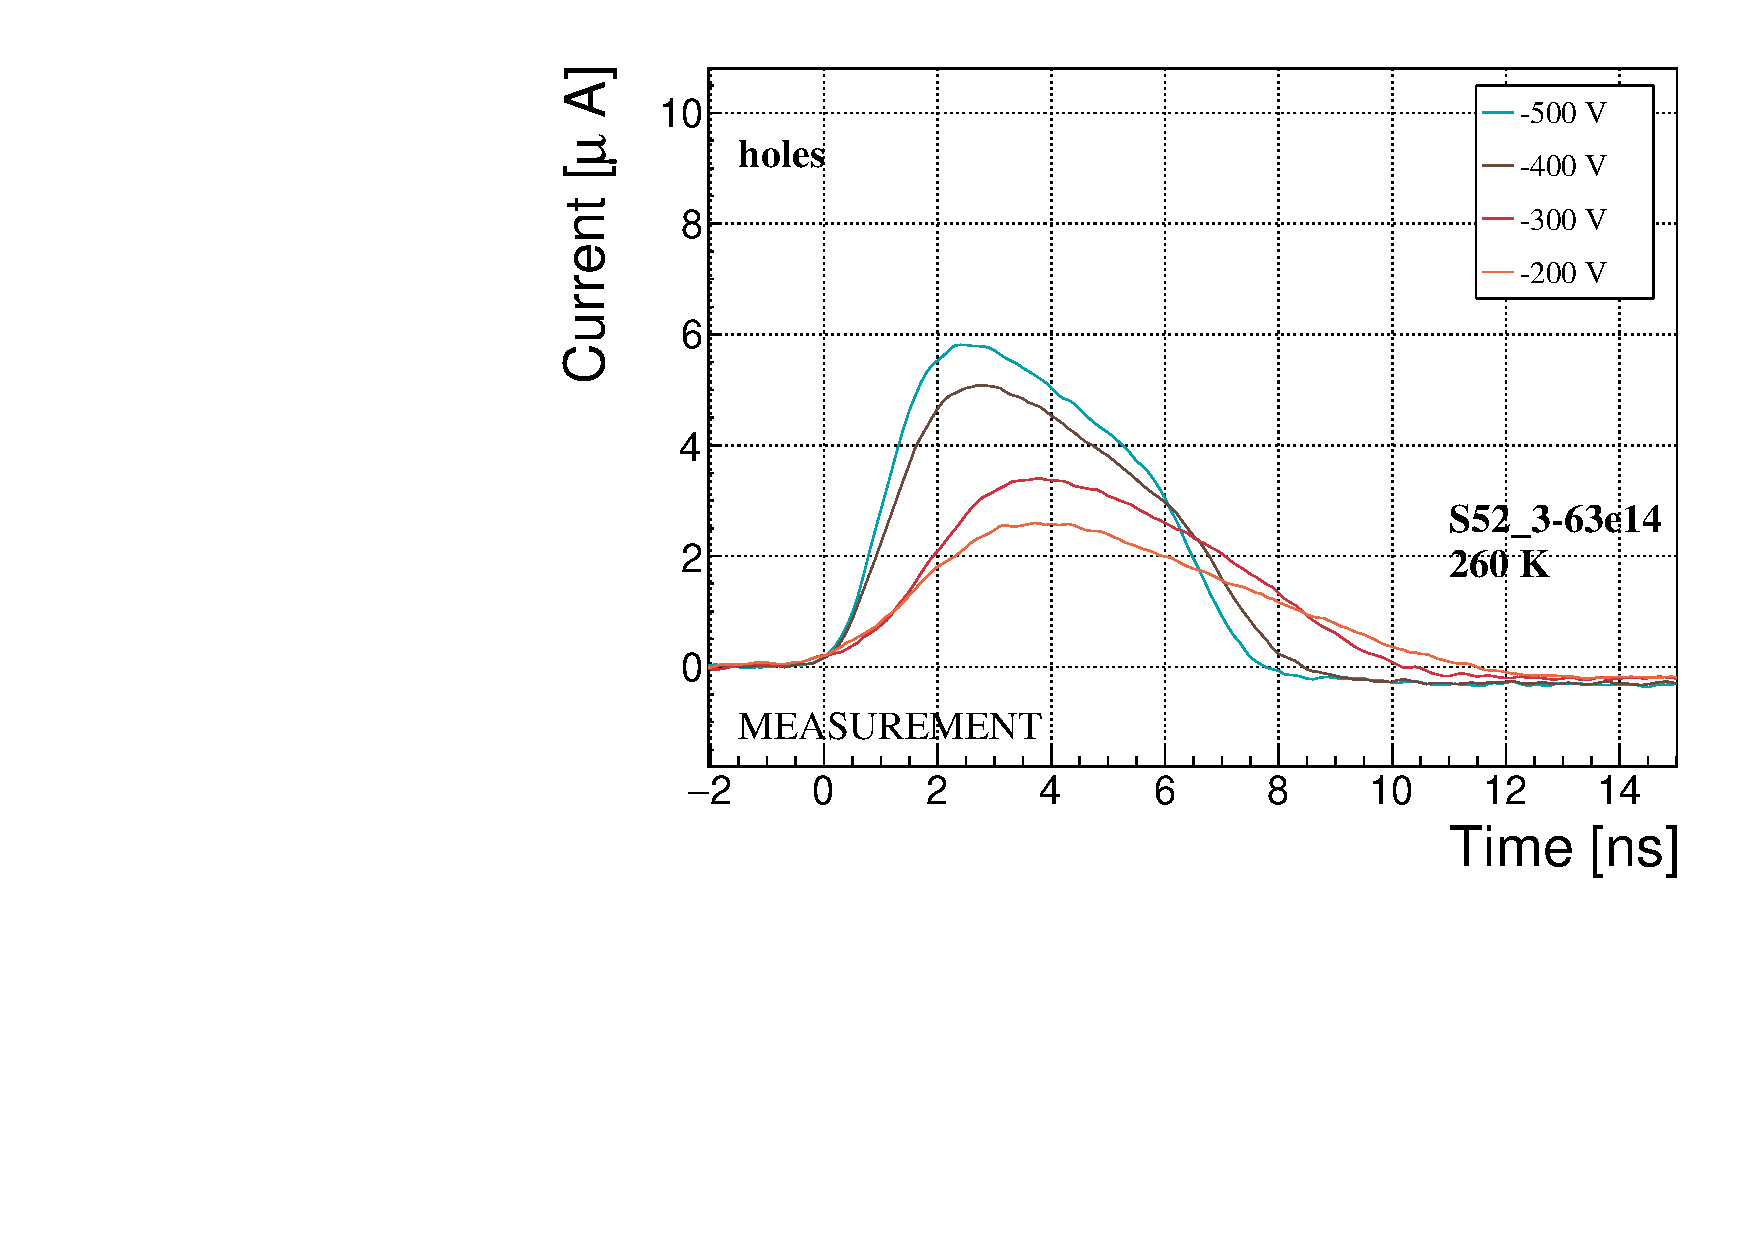
\includegraphics[width=0.47\textwidth]{03_measurement_results/scripts/plots/pulsesVolt/varVolt_S52_3-63e14_holes_260k}  \label{fig:S52ctTminusAfter260}}
\end{tabular}
\caption{Varied bias voltage at a fixed temperature for an irradiated sample}
\label{fig:voltpulseAfter}
\end{figure}


Figure~\ref{fig:temppulsesAfter} shows the irradiated S52 and S79 as well as the non-irradiated S37 for comparison, all at a bias voltage of $\pm$500~V and at several temperature points between 4~K and RT. It is evident that the radiation damage affected the shape of the pulses across all temperatures. 


\begin{figure}[!t]
\begin{tabular}{rr}
\subfloat{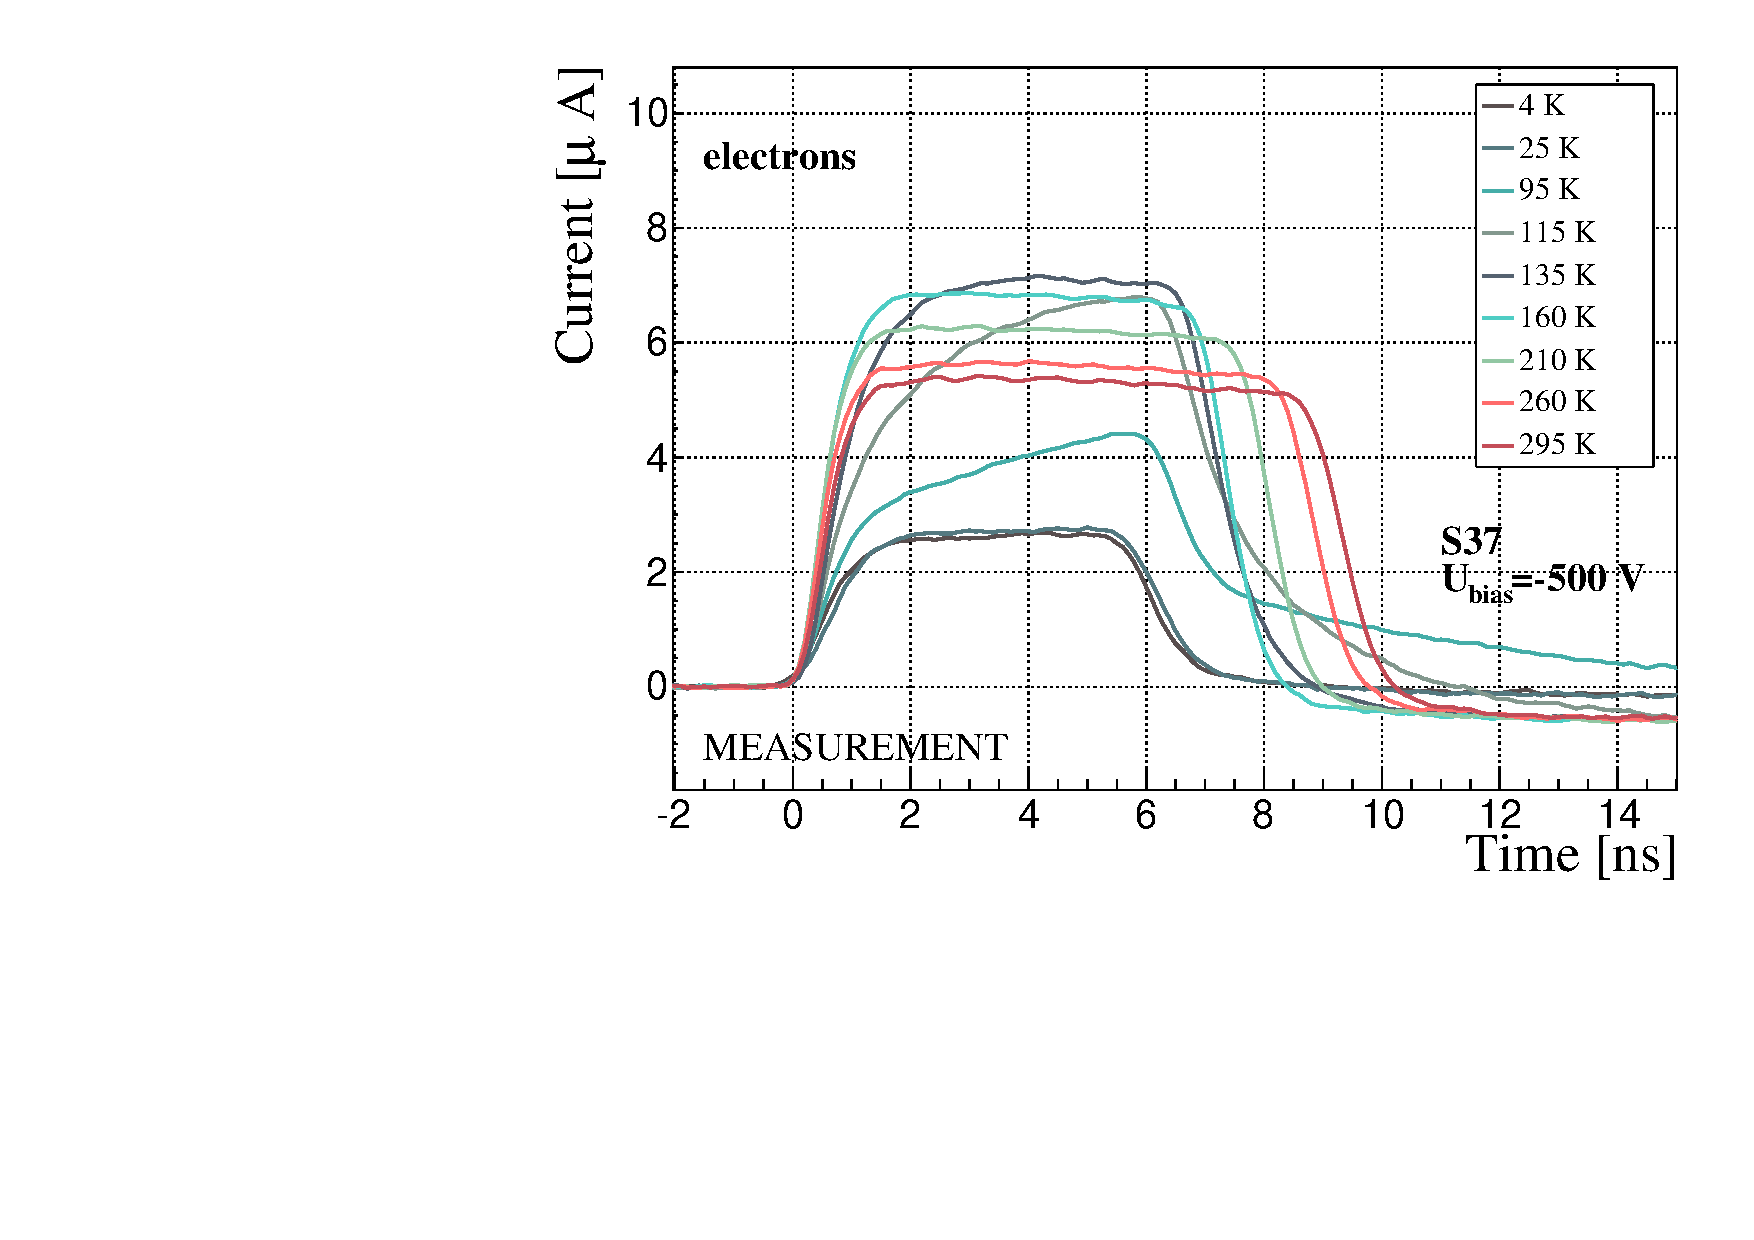
\includegraphics[width=0.47\textwidth]{03_measurement_results/scripts/plots/pulses/S37_elecs} \label{fig:S37plusAfter}} &
\subfloat{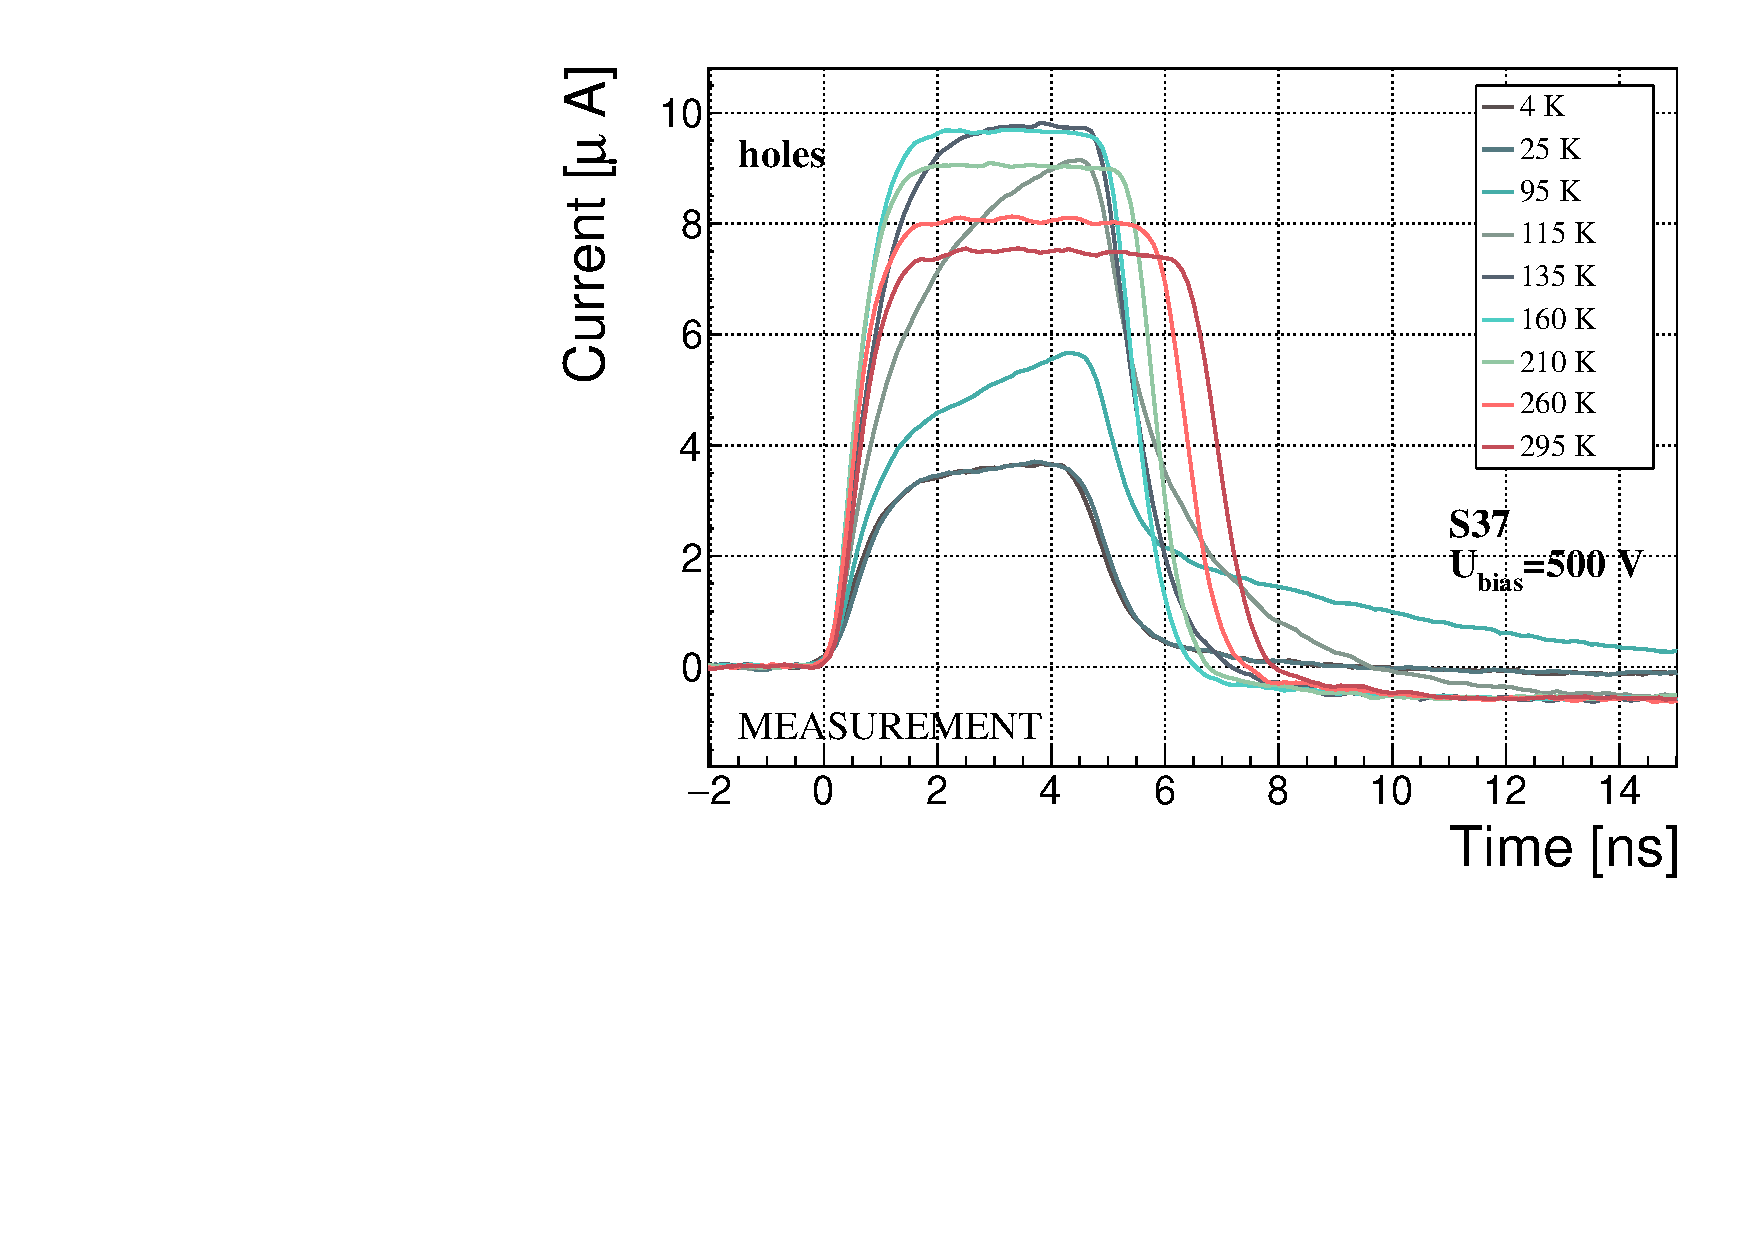
\includegraphics[width=0.47\textwidth]{03_measurement_results/scripts/plots/pulses/S37_holes}  \label{fig:S37minusAfter}} \\
\subfloat{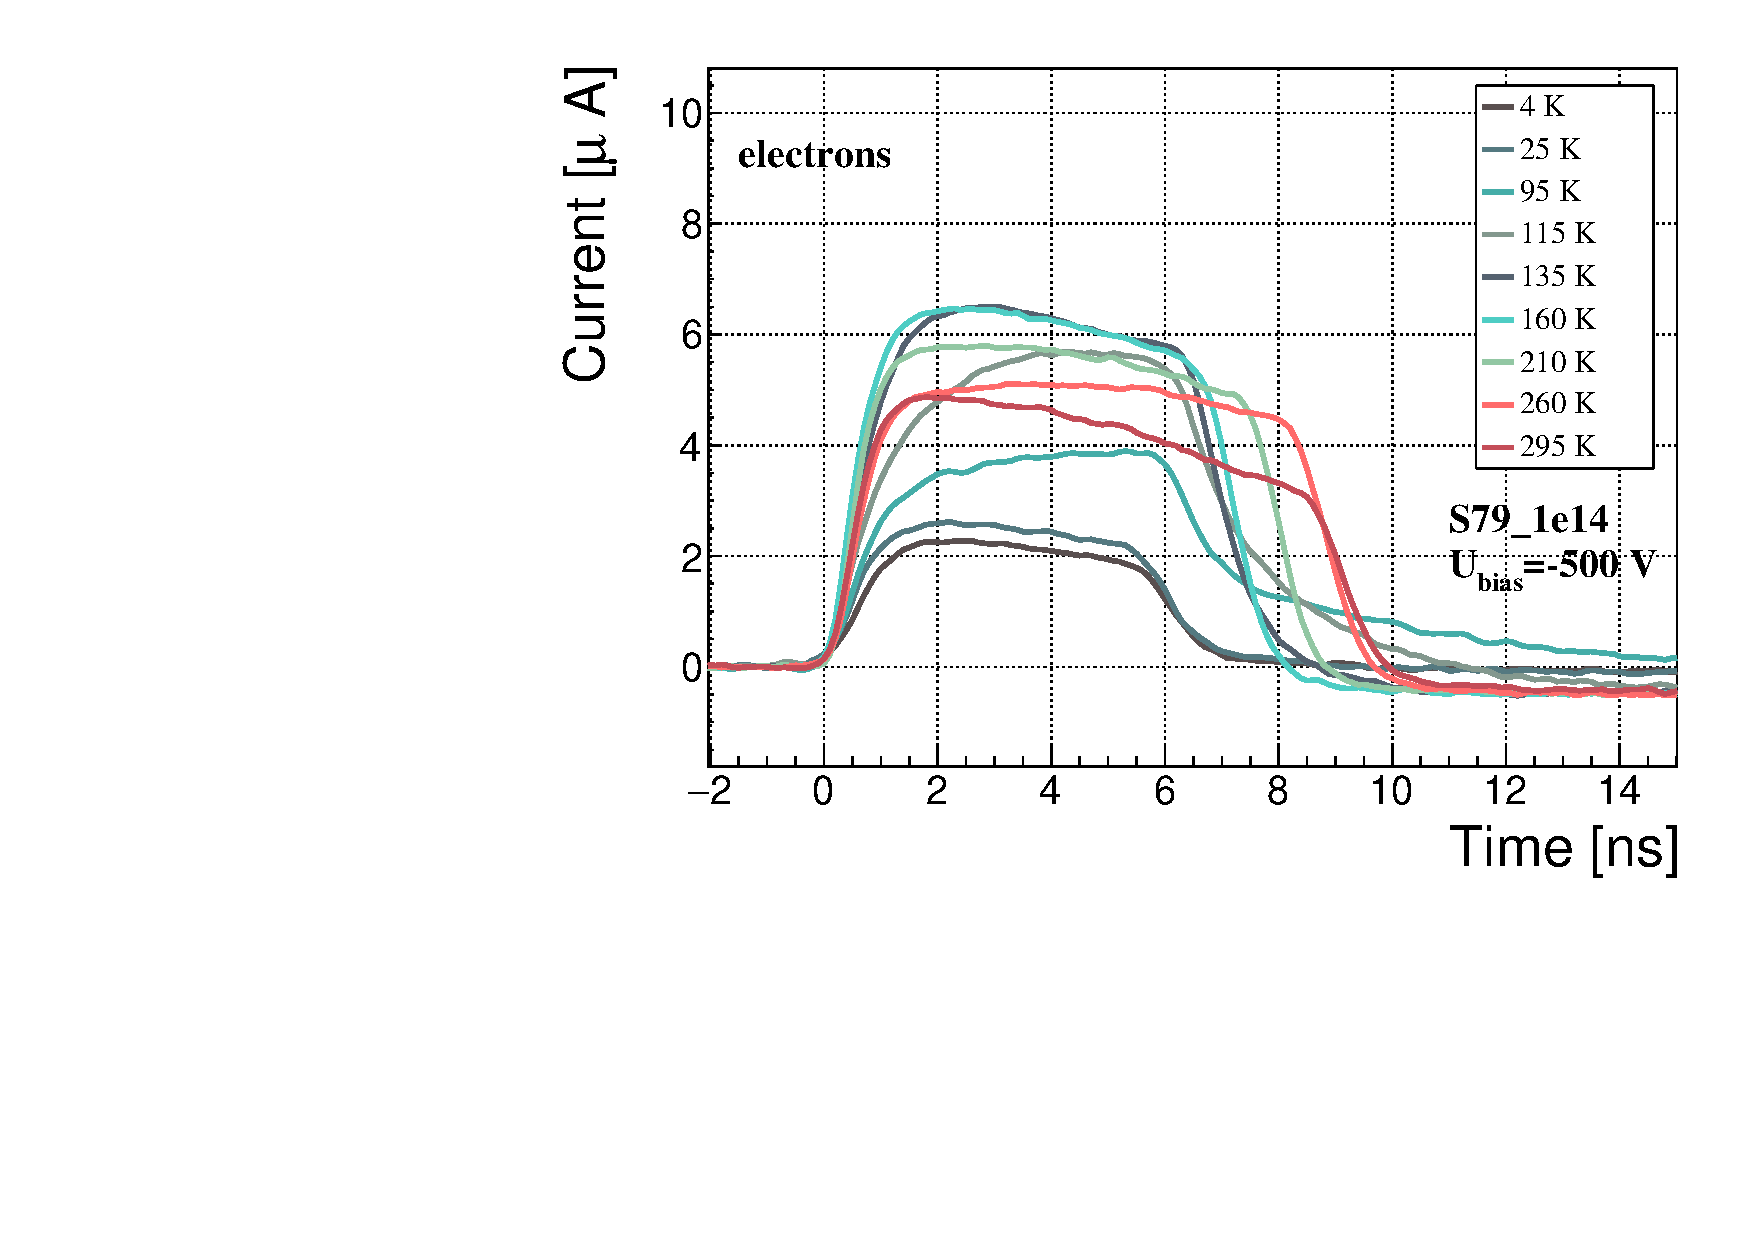
\includegraphics[width=0.47\textwidth]{03_measurement_results/scripts/plots/pulses/S79_1e14_elecs} \label{fig:S79plusAfter}} &
\subfloat{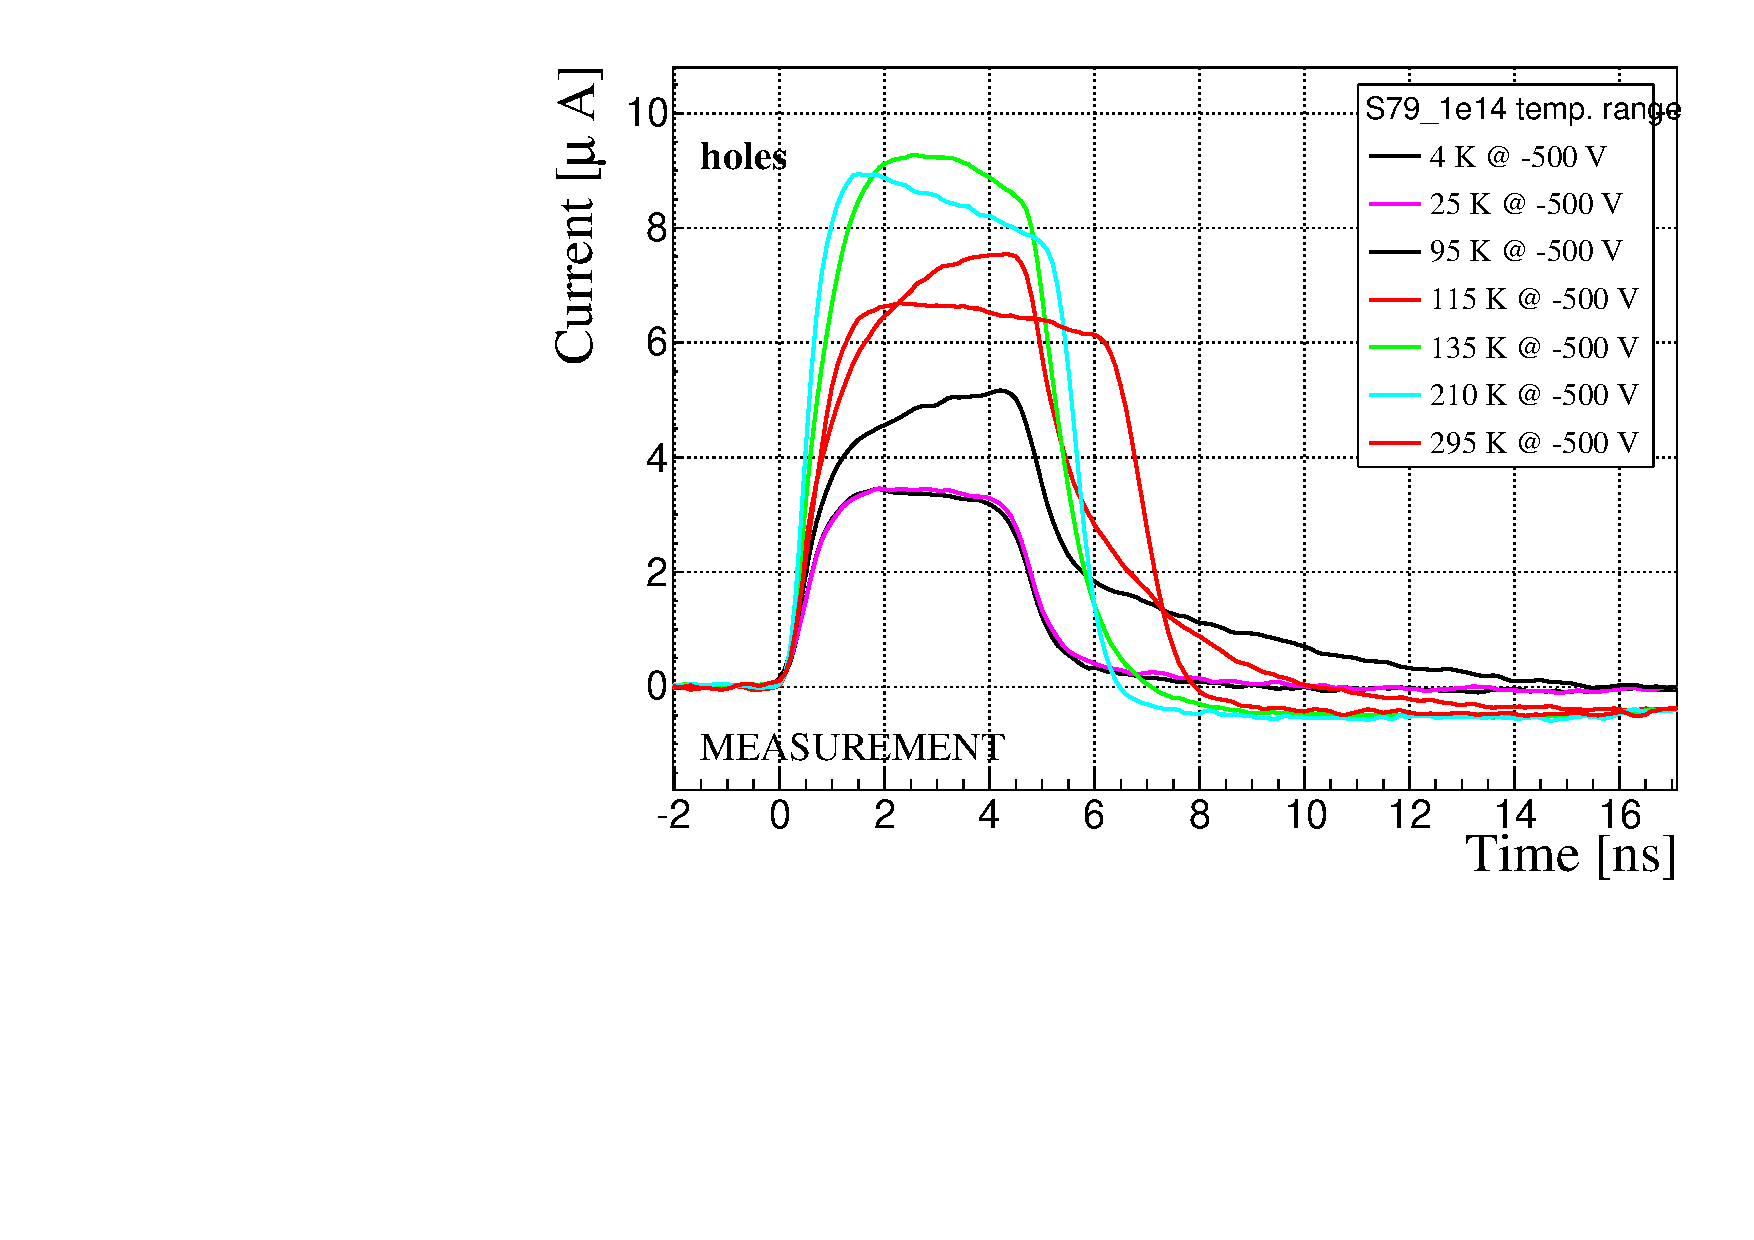
\includegraphics[width=0.47\textwidth]{03_measurement_results/scripts/plots/pulses/S79_1e14_holes}  \label{fig:S79minusAfter}} \\
\subfloat{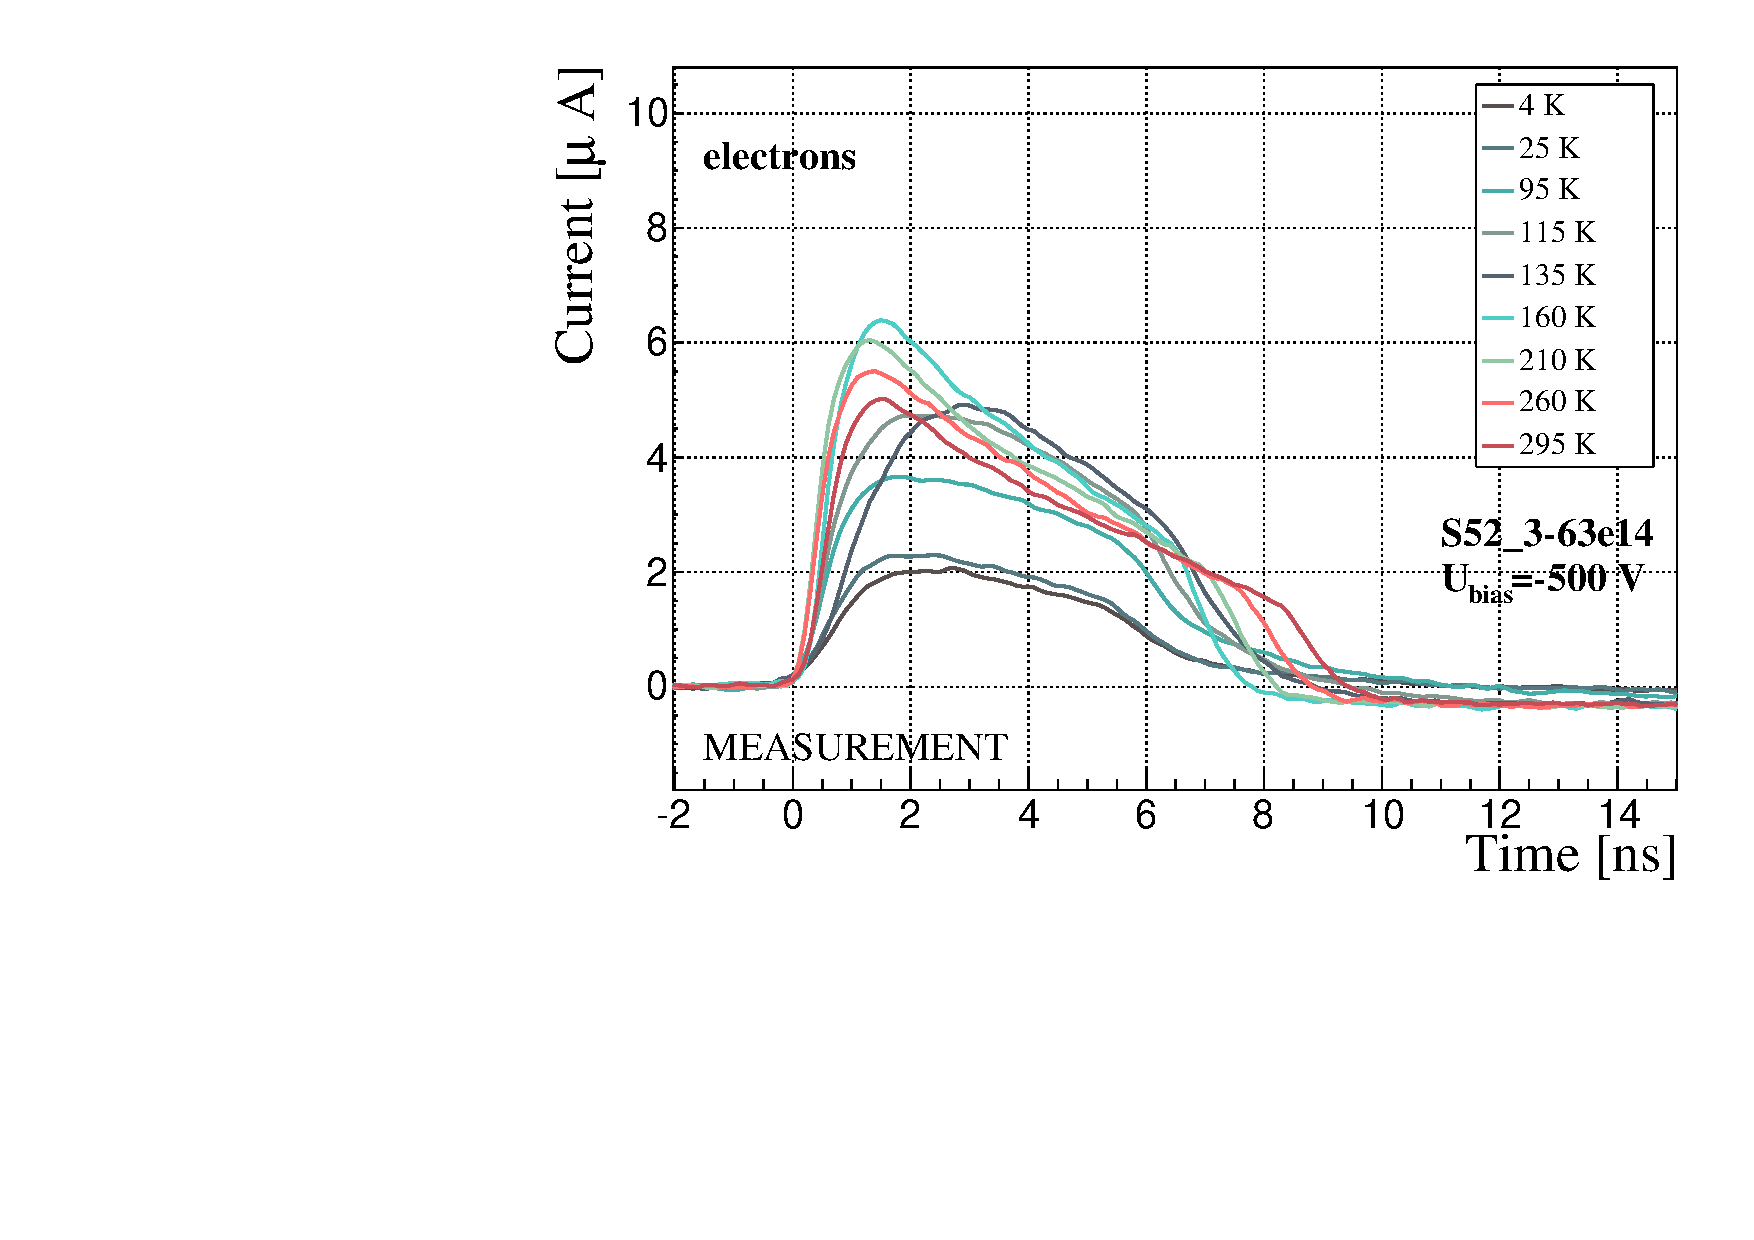
\includegraphics[width=0.47\textwidth]{03_measurement_results/scripts/plots/pulses/S52_3-63e14_elecs} \label{fig:S52plusAfter}} &
\subfloat{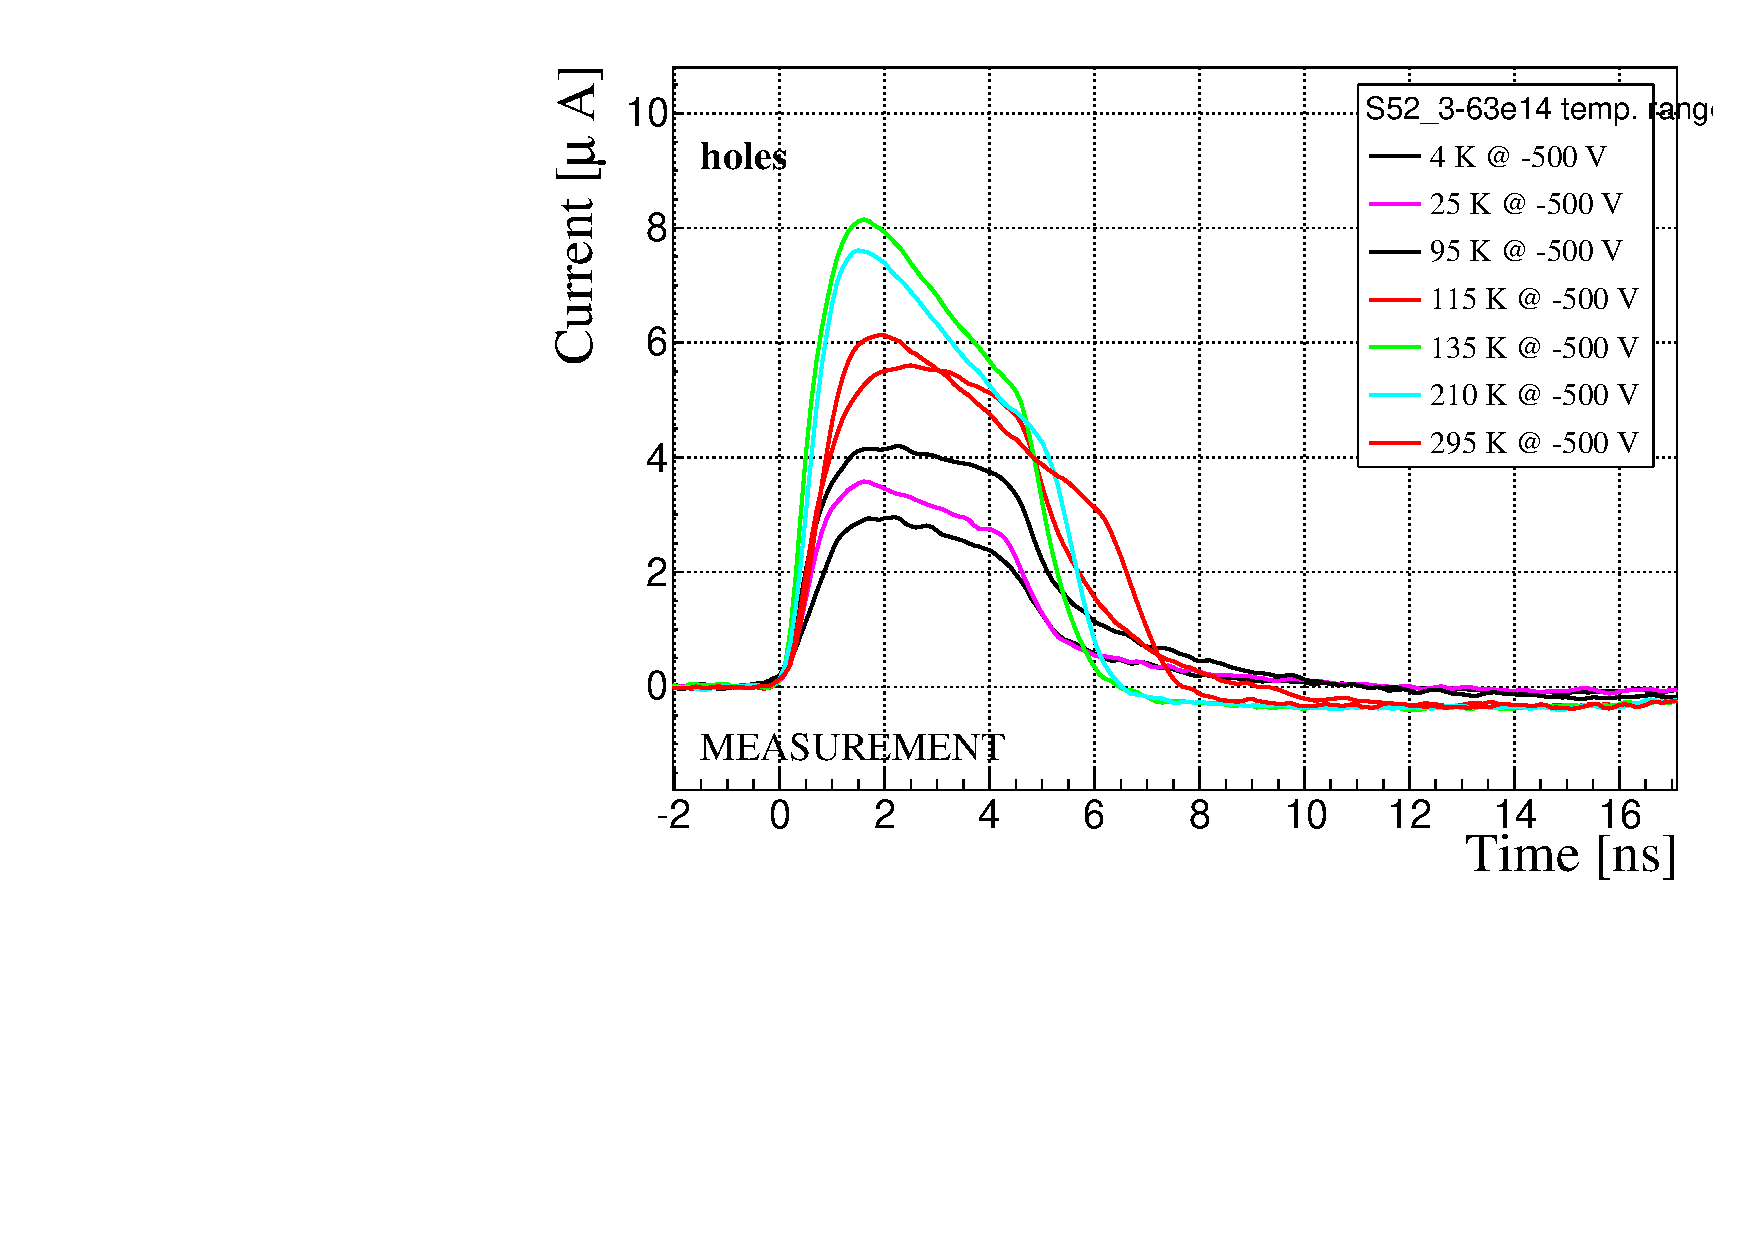
\includegraphics[width=0.47\textwidth]{03_measurement_results/scripts/plots/pulses/S52_3-63e14_holes}  \label{fig:S52minusAfter}}
\end{tabular}
\caption{After irradiation: several data points between 4~K and 295~K at a bias voltage of $\pm$500~V}
\label{fig:temppulsesAfter}
\end{figure}


\subsubsection{Collected charge as a function of temperature}
The area below the current pulse is proportional to the charge collected by the diamond detector. The collected charge is observed as a function of temperature. First, the amplitude values of the averaged pulses at a bias voltage of $\pm$500~V and across the temperature range between 4~K and 295~K have to be integrated. Then a calibration factor is used to derive the charge for all data points. This factor is obtained using a Cx charge-sensitive amplifier. The resulting values for electrons and holes are plotted in figures~\ref{fig:chgtempelecs} and~\ref{fig:chgtempholes}, respectively. Thesis~\cite{Jansen:1956431} gives a model that explains the drop in charge below 150~K. The new contribution are the data points for the irradiated samples. The values for them are lower than the those of non-irradiated samples, which is expected.

The values for all samples are fairly stable in the range between 4~K and 75~K and between 150~K and 295~K. However, in the values for the irradiated S52 some excursions can be observed. This is due to the sequence of the measurement steps, which introduced a hysteresis effect and is explained in the preceding text.

The collected charge drops significantly from 150~K down to 75~K. In the non-irradiated samples the values in the lower temperature range are approximately 0.30 of the values at the high range. For the irradiated ones this difference is lower -- a factor of 0.35 for S79 and 0.5 for S52. An interesting detail is that the ratio between the values for non-irradiated samples and their irradiated counterparts  at the lower range is different than at the higher range. Looking at the values for the electron collection in figure~\ref{fig:chgtempelecs}: for S52 the lower ratio is equal to 1.28 and the higher equal to 1.7. For S79 these ratios are 1.00 and 1.09, which means that the difference in charge collection between 4~K and 75~K before and after irradiation is negligible.

\begin{figure}[!t]
\centering
\begin{tabular}{cccc}
\subfloat{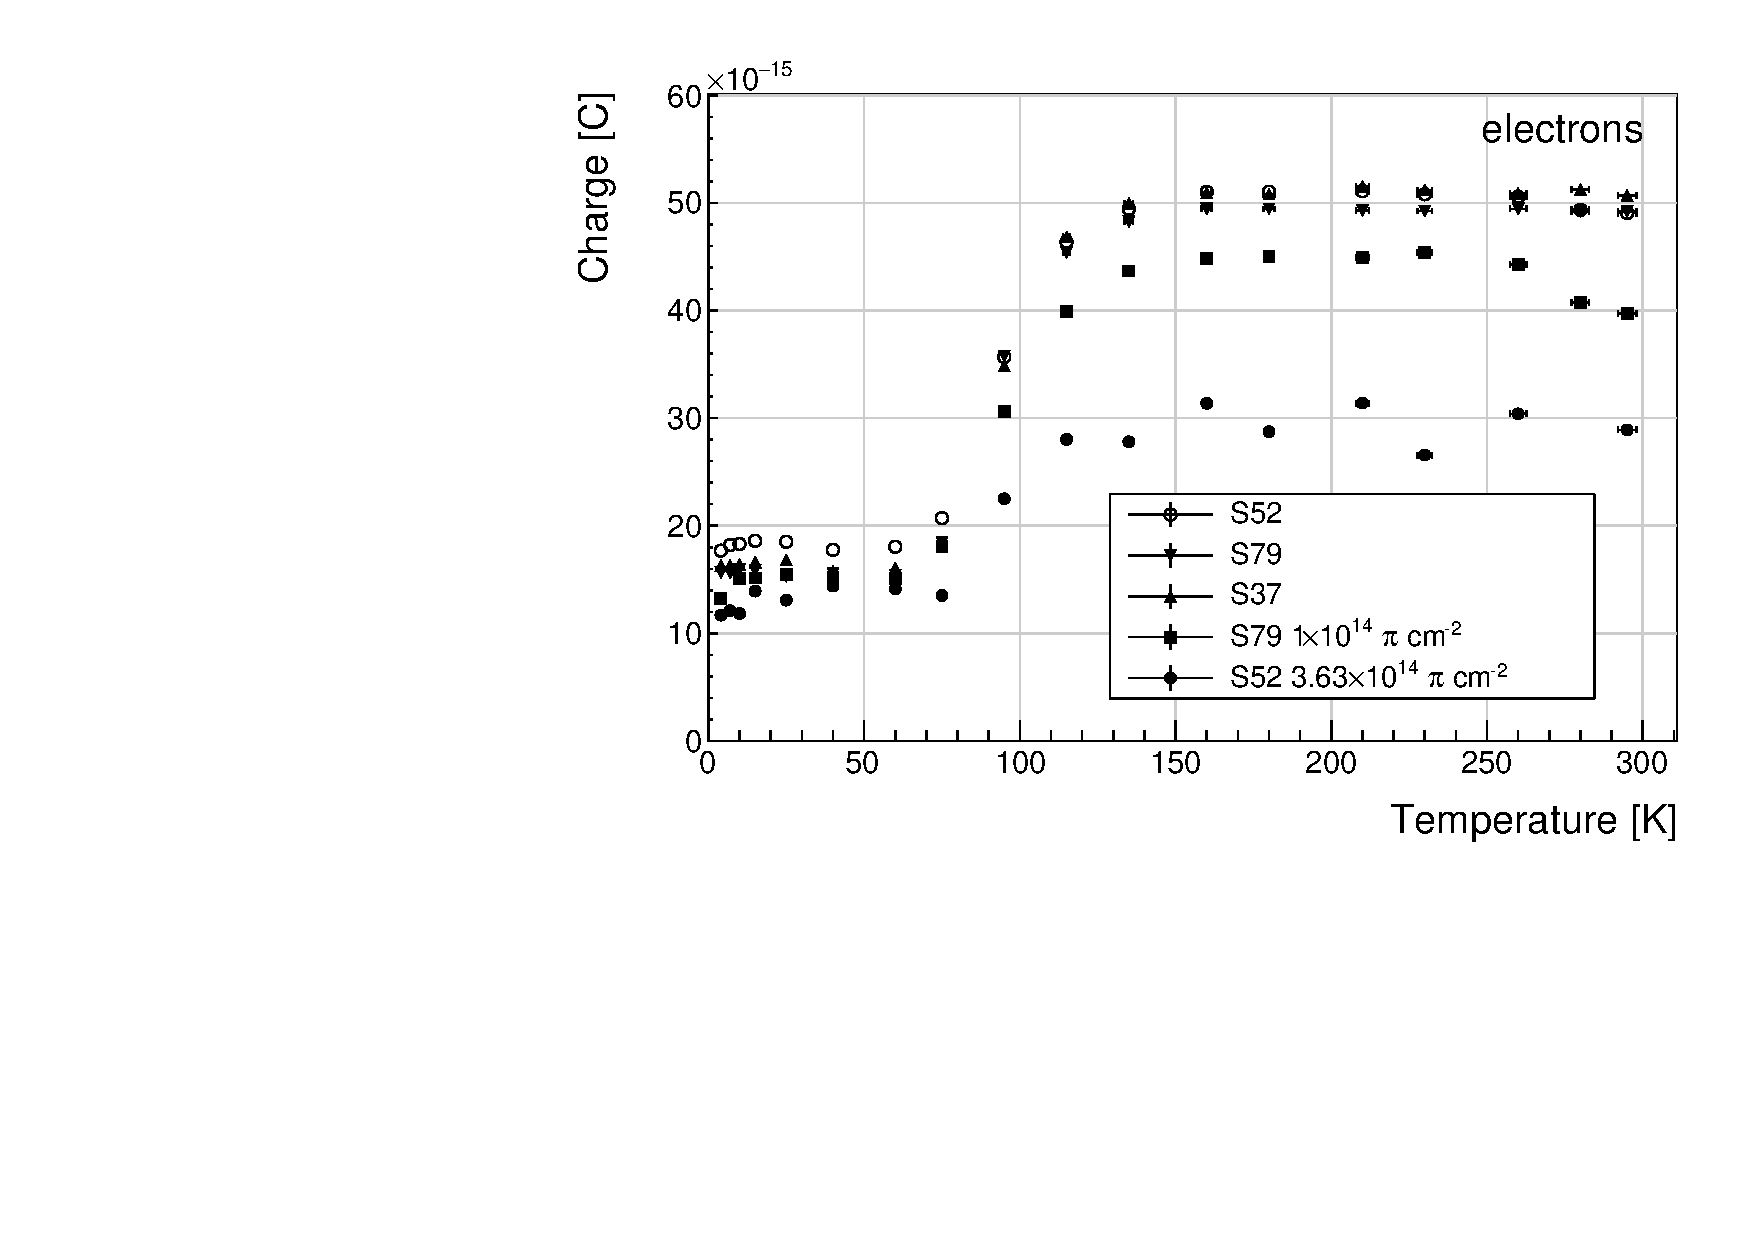
\includegraphics[width=0.80\textwidth]{03_measurement_results/scripts/plots/charge500V} \label{fig:chgtempelecs}} \\
\subfloat{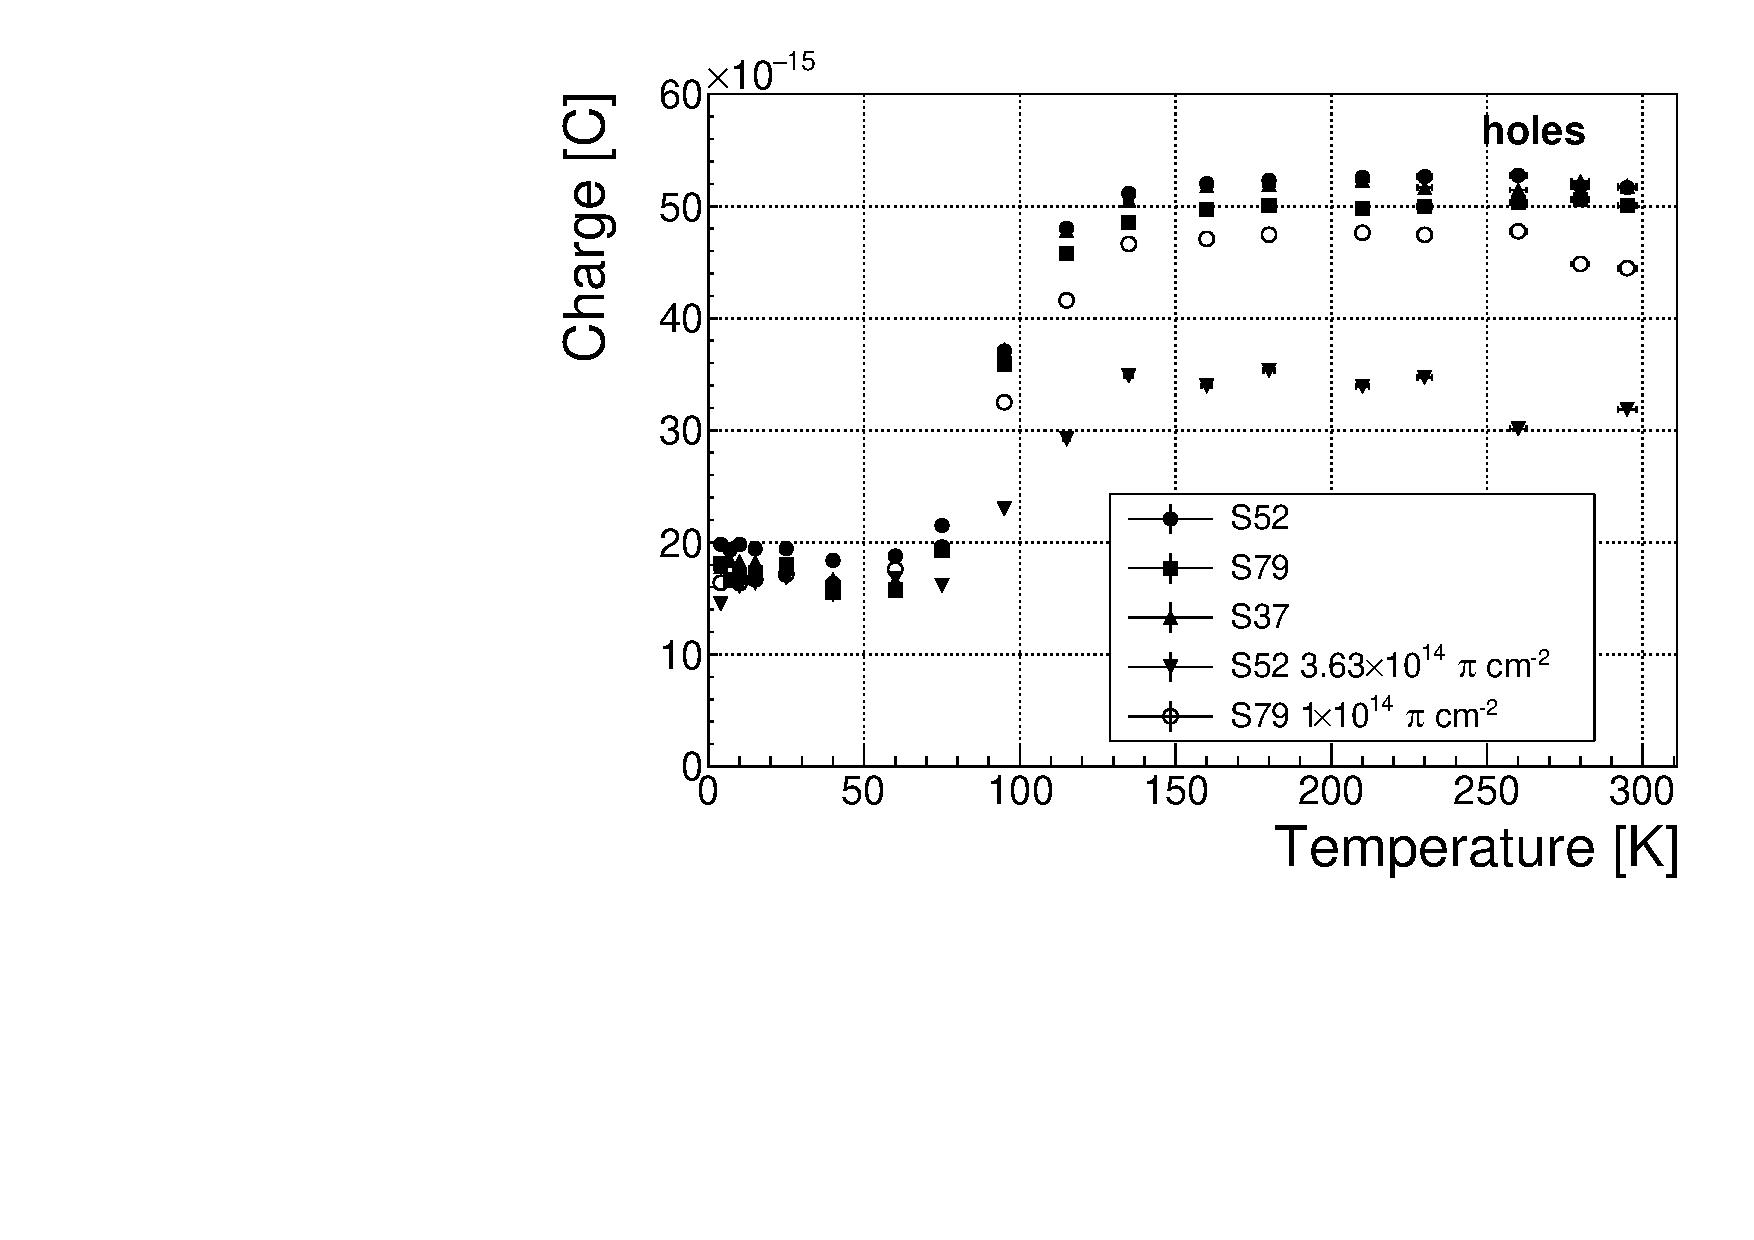
\includegraphics[width=0.80\textwidth]{03_measurement_results/scripts/plots/charge-500V}  \label{fig:chgtempholes}}
\end{tabular}
\caption{Collected charge as a function of temperature}
\label{fig:chgtemp}
\end{figure}



\subsubsection{Charge trapping}
The carriers drifting through the bulk get stopped by the charge traps with a certain probability. This trapping happens uniformly throughout the diamond, decreasing the number of carriers in the charge cloud. Therefore the absolute number of trapped carriers decreases. At the same time the absolute number of trapped carriers per unit of length decreases. The resulting function for the number of drifting carriers per unit of length is a decaying exponential function:
\begin{equation}
\label{eq:decayexp}
I(t)=I(0) \cdot e^{-\frac{t-t_0}{\tau} } + I_0,
\end{equation}
where $I(0)$ is the initial induced current, $I_0$ is the end current, $t$ is time, $t_0$ is temporal displacement of the pulse and $\tau$ is the decay time constant. This value tells how long it takes before the amplitude of the pulse decreases to 63~\% of its initial height.

The decaying exponential function has been fitted to the decaying top of the averaged pulses at bias voltages of $\pm$400~V and $\pm$500~V across all temperatures excluding the transitional range between 75~K and 150~K. The resulting decay time constants $\tau$ for an individual temperature point are not equal, which stems from the fact that the pulses change with time due to ``polarisation''. This counts as a systematic error. Therefore the fitted $\tau$ for $\pm400$~V and $\pm500$~V are averaged into one value representing the measurement at that temperature point. Figure~\ref{fig:lifetimevstemp} shows the fitted $\tau$ for the five samples between 4~K and 295~K. In principle, the time constants should be infinite for a perfect and non-irradiated sample. Here a slightly tilted top of the pulse due to space charge is already successfully fitted with an exponential function, resulting in a $\tau$ of the order of (200$\pm$20)~ns$^{-1}$. Consequently the fitting method is not adequate for non-irradiated samples. For the irradiated samples, the fit becomes increasingly more meaningful. As seen in figure~\ref{fig:lifetimevstemp}, the fitted values of the irradiated samples are fairly stable across all temperatures. There is a slight increase in the decay time constant of the S52 from $(6.0\pm0.5)$~ns$^{-1}$ above 150~K to ($8.5\pm0.9$)~ns$^{-1}$ below 75~K. On the other hand, this step is not observable in the S79 data. With only one sample exhibiting this behaviour, the effect is not significant enough. Judging by the data acquired, the samples would need to be irradiated to doses above $1\times10^{14}~\uppi~$cm$^{-2}$ to quantify this effect in detail. So far this effect will not be regarded as significant for the scope of this thesis. Building on this assumption, the conclusion is that the signal decay time constant for irradiated sCVD diamond is constant across the temperature range between 4~K and 195~K, excluding the transitional range between 75~K and 150~K. 

Taking into account the conclusions above, all the values can be averaged into one decay constant. Figure~\ref{fig:lifetimevsdose} shows these values for all samples as a function of the received $\uppi_\mathrm{300~MeV}$ radiation dose. To estimate the carrier lifetime with respect to the radiation dose received, a similar model is used than that in section~\ref{sec:radlimit}. This model states that the inverse of the carrier lifetime is linearly decreasing with increasing radiation dose:
\begin{equation}
\label{eq:ltfactor}
\frac{1}{\tau} = \frac{1}{\tau_\mathrm{0}}+\kappa_{\mathrm{\tau}}\cdot\Phi
\end{equation} 
\begin{equation}
\label{eq:ltfactor1}
\tau = \frac{\tau_\mathrm{0}}{\kappa_{\mathrm{\tau}} \tau_\mathrm{0} \Phi + 1}
\end{equation} 
where $\tau_\mathrm{0}$ is the lifetime for a non-irradiated sample (real lifetime, therefore of the order of 400~ns$^{-1}$), $\tau$ is the lifetime of an irradiated sample, $\Phi$ is the received radiation dose and $\kappa_{\mathrm{\tau}}$ the lifetime degradation factor. For these data the fitted factor is equal to $\kappa_{\mathrm{\tau}}=(3.6\pm0.8)\times10^{-16}~$s~cm$^2$~$\uppi_{\mathrm{300~MeV}}^{-1}$. Using this factor, the steepness of the decay in the pulse shape with respect to radiation dose can be estimated. This can help when designing a system where current pulse shape is an important factor.
%introduce the kTau factor

\begin{figure}[!t]
\centering
\begin{tabular}{cccc}
\subfloat
{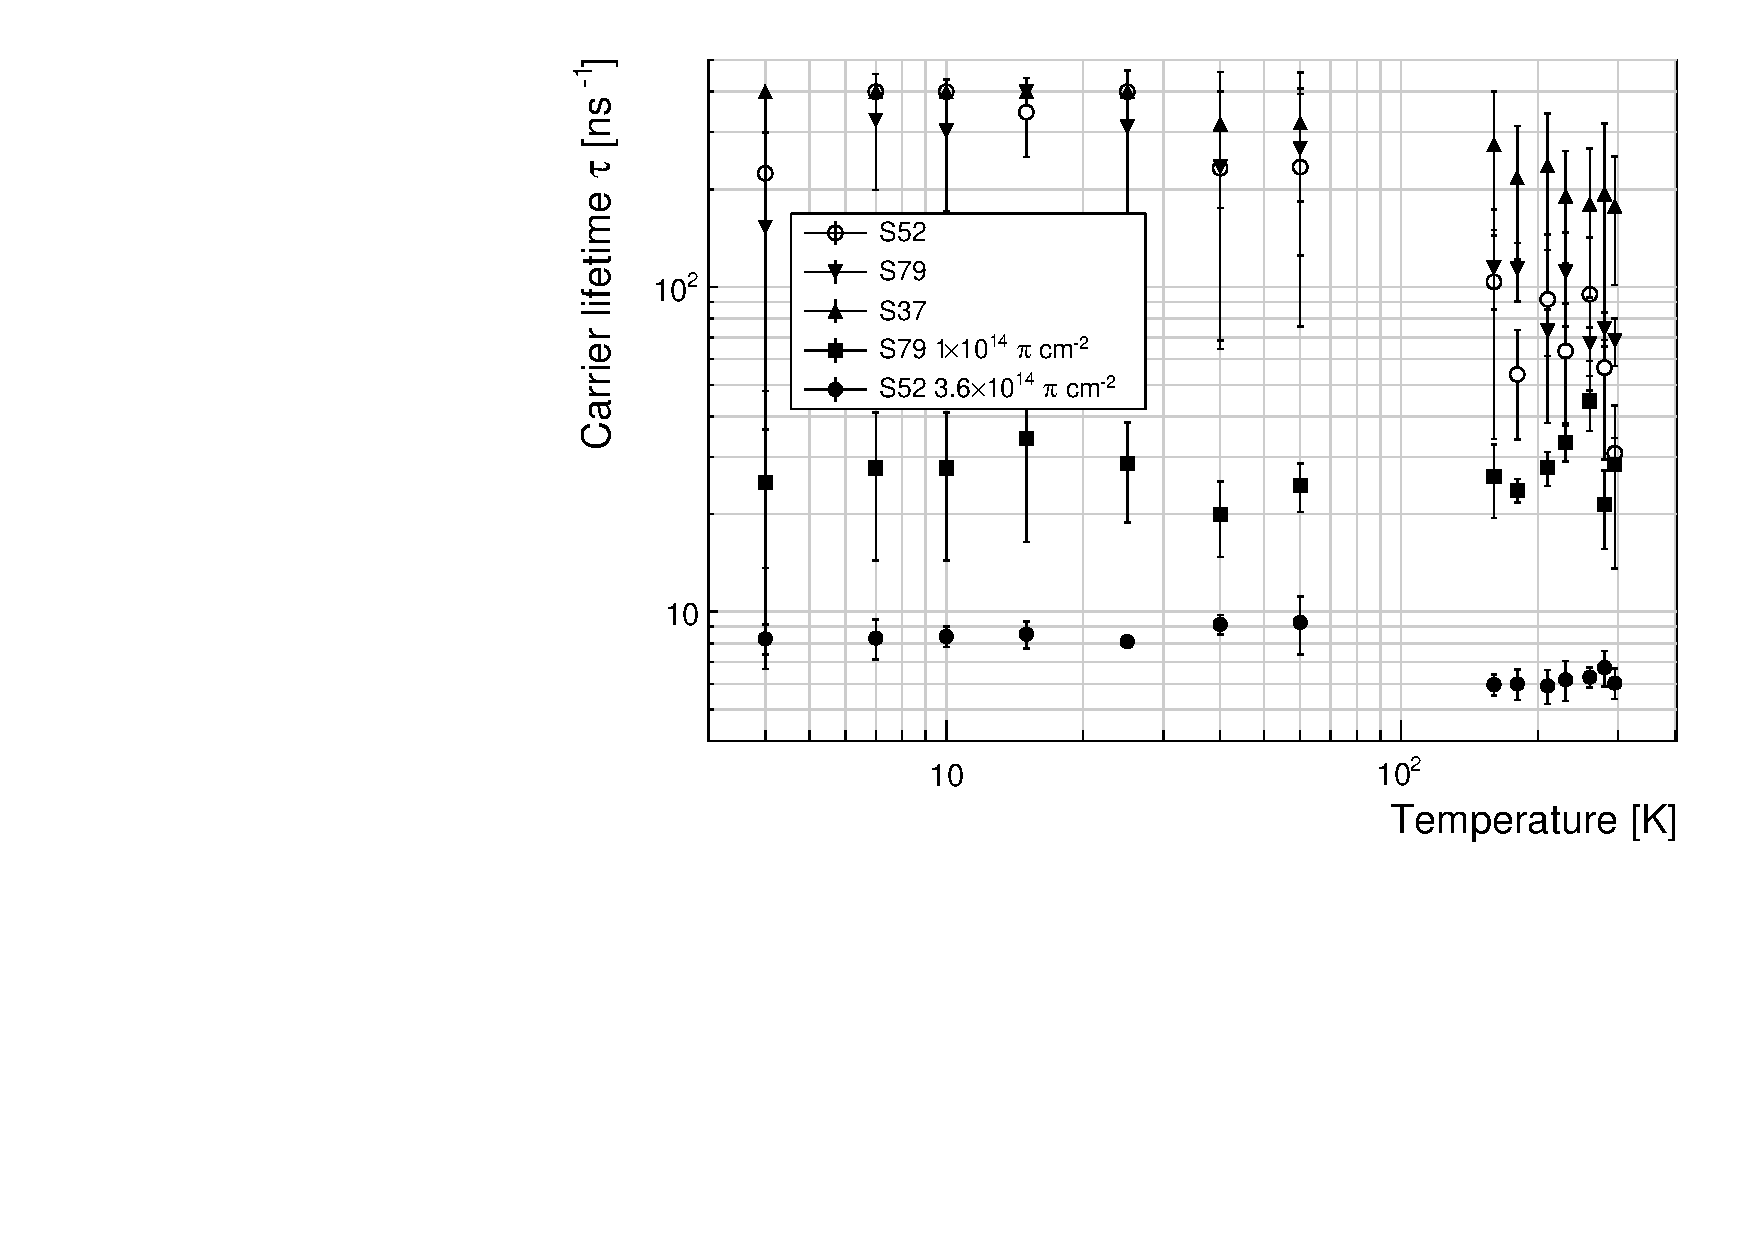
\includegraphics[width=0.8\textwidth]{03_measurement_results/scripts/plots/taunew/lifetimevstemp} \label{fig:lifetimevstemp}} \\
\subfloat
{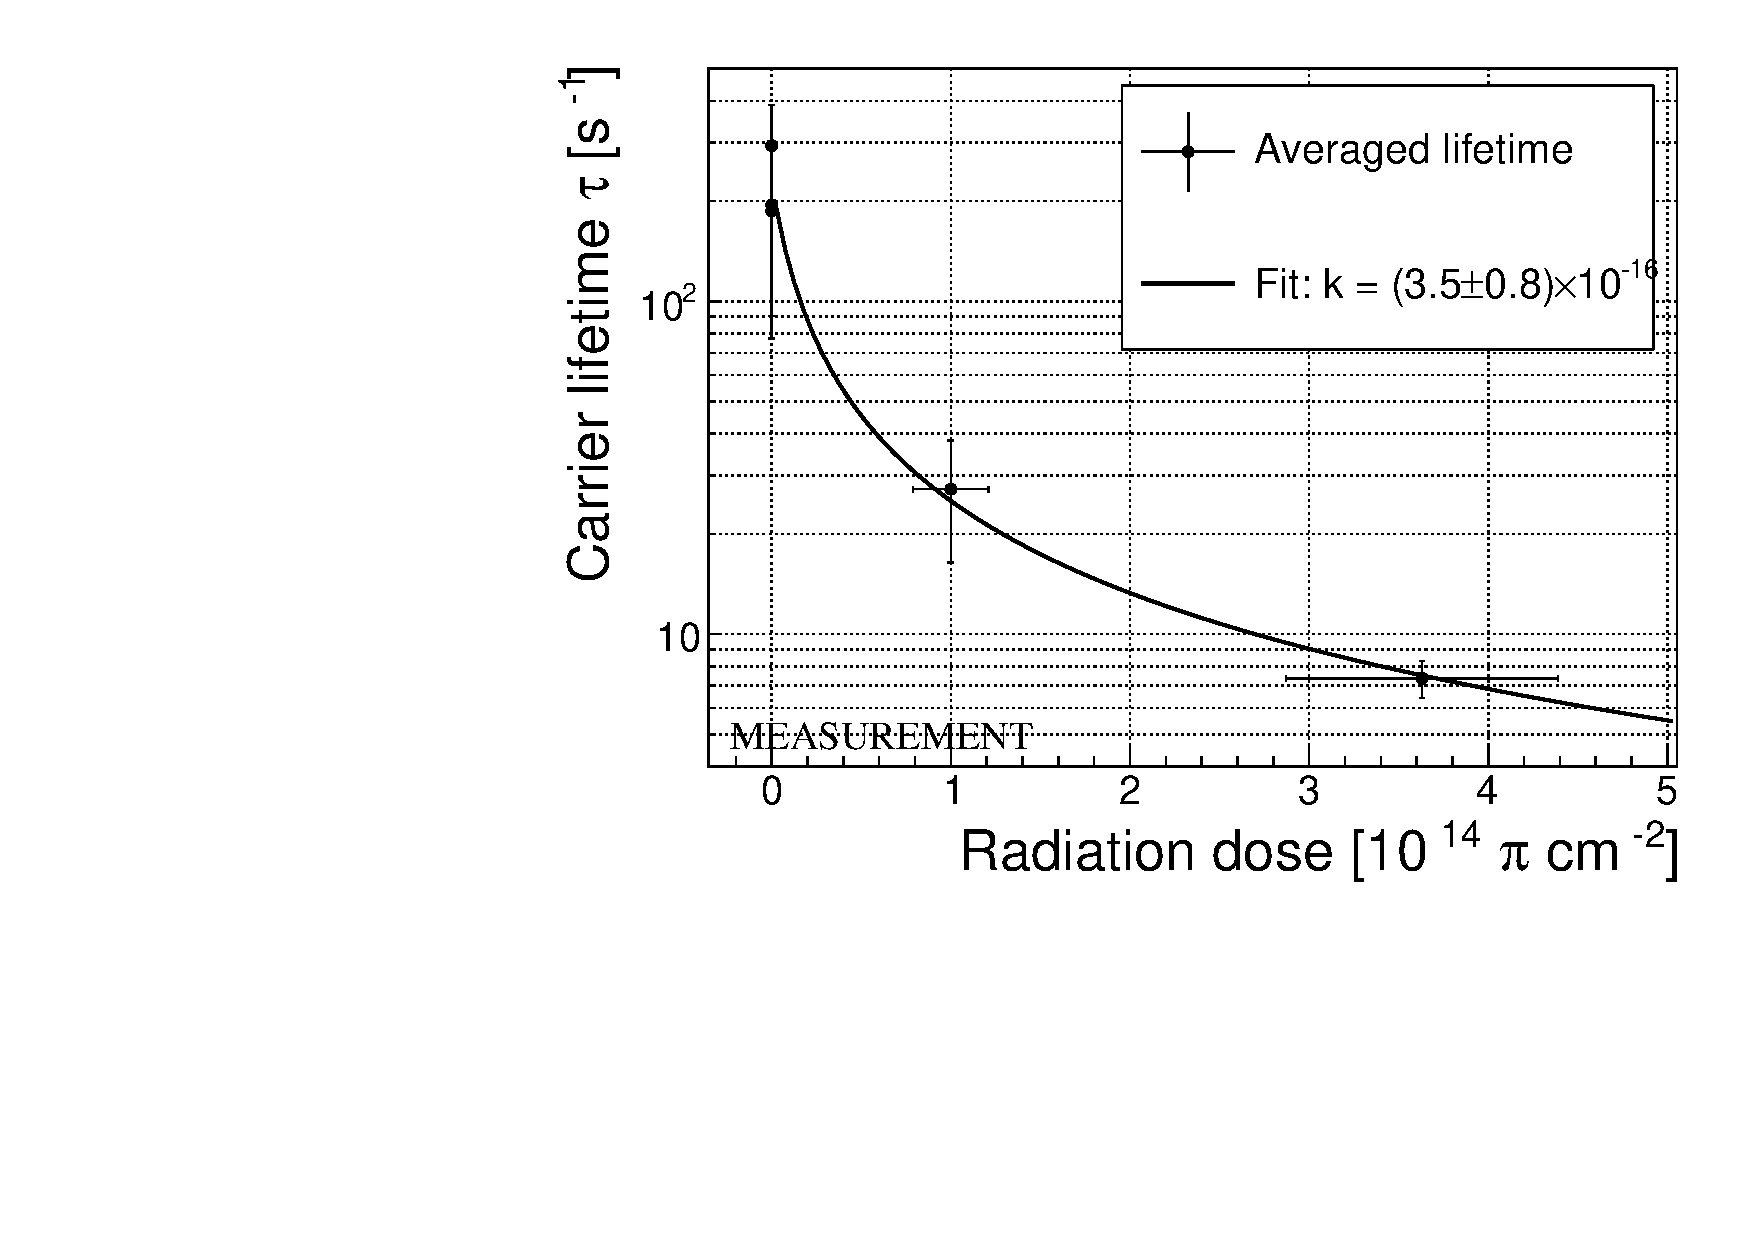
\includegraphics[width=0.8\textwidth]{03_measurement_results/scripts/plots/taunew/avglifetime}  \label{fig:lifetimevsdose}}
\end{tabular}
\caption{Charge carrier lifetime decreases with irradiation, but is stable across the range of temperatures between 4~K -- 75~K and 150~K -- 295~K. The first figure shows the carrier lifetime s a function of temperature whereas the second figure depcits the carrier lifetime averaged over all temperatures and plotted against the $\pi$ irradiation dose}
\label{fig:carrlifetime}
\end{figure}










% ---------------------------------------------------------------------------------------------------------------
\clearpage
\section{Conclusion}
\label{sec:radlimit}
% ---------------------------------------------------------------------------------------------------------------
This chapter gives an overview of the capabilities and limitations of diamond as a particle detector. Three effects on diamond were studied -- noise, radiation and temperature, the focus being on the latter two. 

Two sCVD diamond detectors were irradiated with 300~MeV pions. They were tested alongside a non-irradiated sample to observe the changes in the ability to detect $\upalpha$, $\upbeta$ and $\upgamma$ radiation. Their charge collection efficiency was measured in a test beam facility using . The results were compared to the results from the RD42 collaboration and a DPA model. A radiation damage factor $k_{\mathrm{\lambda}}=(3.0\pm1.0)\times10^{-18}~\upmu$m$^{-1}$~cm$^{-2}$ was obtained for $\uppi_{\mathrm{300~MeV}}$ particles. The data point was not in agreement with the data provided by RD42 nor with the model. However, the irradiation process and the low number of tested samples hold a relatively high statistical uncertainty. In addition, there was no diamond surface treatment done in between the measurements, as is the case in the study conducted by RD42. The results obtained in the course of these measurements will also be fed into the existing pool of data in the RD42 collaboration.

The next step was to test the long-term capabilities for $\upalpha$ detection. The shape of the ionisation profile was investigated to determine the behaviour of the charge carriers in the irradiated diamond. An exponential decay was observed in the pulses of irradiated samples, proving that there are charge traps in the bulk that were created during irradiation. Then a long-term stability test was carried out. The results show that the irradiated diamond detectors do not provide a stable and reliable long-term measurement of $\upalpha$ particles. This might be due to a space-charge build-up in the bulk, which changes the electric field, affecting the charge carriers. A procedure to improve the pulse shape using $\upbeta$ and $\upgamma$ radiation was proposed.

Finally, the diamond sensors were cooled down to temperatures between 4~K and 295~K. Their response to $\upalpha$ particles was observed. The results of the non-irradiated and irradiated samples were compared. The effect of reduction for the number of drifting charges due to exciton recombination was observed in both sets of data. The second set had a superimposed effect of charge trapping during the drift, which was represented by an exponential decay in the signal. The decay time constant did not change with temperature. Therefore all temperature points for individual samples were averaged and the decay time constants were plotted against the received radiation dose. A damage factor equal to $\kappa_{\mathrm{\tau}}=(3.5\pm0.8)\times10^{-16}$~s~cm$^2$~$\uppi_{\mathrm{300~MeV}}^{-1}$ for non-primed diamonds was defined.
